\chapter[广义非线性分数Schr{\"o}dinger波方程的任意高阶显式能量守恒方法]{广义非线性分数Schr{\"o}dinger波方程的任意高阶显式能量守恒方法
}
\section*{摘要}

本文引入了一种新颖的显式守恒数值方法类别,该方法的阶数可任意升高,用于解决一维和二维非线性分数Schr{\"o}dinger波方程。本研究所提出的方法基于标量辅助变量的思想。首先通过引入标量辅助变量,将研究对象的方程转化为一个等效的系统,随后将能量重新表述为三个二次项的总和。
在时间上,我们采用显式松弛Runge-Kutta方法,在空间上使用傅立叶拟谱离散化。经证明,由此产生的时空全离散方案在离散层面上能够保持重新表述的能量,精度达到机器精度。所提出的方法在长期计算中显著提升了数值稳定性,这一点通过数值实验证实。
值得注意的是,这一思想也可以轻松推广到其他类似的方程,如非线性分数波动方程和分数Klein-Gordon-Schr{\"o}dinger方程。
\section{引言}
这篇论文关注于非线性分数Schr{\"o}dinger波方程(NFSWEs)初边值问题的数值解,其方程形式如下:
\begin{align}
&  u_{t t}+(-\Delta)^{\alpha / 2} u+\mathrm{i} \kappa u_{t}+\beta g(|u|^{2}) u=0, \quad \boldsymbol{x} \in \Omega, \quad  t \in(0, T],\label{eq_SAVRRK:1}\\
& u(\boldsymbol{x}, 0)=u_{0}(\boldsymbol{x}), \quad u_{t}(\boldsymbol{x}, 0)=u_{1}(\boldsymbol{x}),\quad \boldsymbol{x} \in \Omega, \label{eq_SAVRRK:2}\\
& u(\boldsymbol{x}+\boldsymbol{L}, t)=u(\boldsymbol{x}, t), \quad t \in[0, T],\label{eq_SAVRRK:3}
\end{align}
其中,$\mathrm{i}=\sqrt{-1}$,$1<\alpha \leq 2$,$\kappa, \beta(>0)$为两个实常数,$u(\boldsymbol{x}, t)$是未知的复值函数,$u_{0}(\boldsymbol{x})$ 和 $u_{1}(\boldsymbol{x})$ 为已知的光滑函数,非线性项 $g$ 是给定的实函数,$\boldsymbol{x}\in\Omega\!\subset\!
R^d~(d\!=\!1,2)$,$\boldsymbol{L}$ 是周期。分数拉普拉斯算子可以通过傅里叶变换表示为:
\begin{align}\label{eq_SAVRRK:4}
(-\Delta)^{\frac{\alpha}{2}} u(\boldsymbol{x},t)=\mathcal{F}^{-1}\left[|\boldsymbol{\xi}|^{\alpha} \mathcal{F}(u(\boldsymbol{\xi},t))\right],
\end{align}
其中,$\mathcal{F}$ 和 $\mathcal{F}^{-1}$ 分别表示傅里叶变换及其逆变换,详见 \cite{caffarelliExtensionProblemRelated2007}。NFSWEs \eqref{eq_SAVRRK:1} 可以被看作是经典Schr{\"o}dinger波方程的推广,后者在等离子体中的Langmuir波包络近似等物理应用中具有广泛应用 \cite{colinSemidiscretizationTimeNonlinear1998},并且已经得到深入研究,例如见 \cite{zhangConservativeNumericalScheme2003,baoUniformErrorEstimates2012,chengSeveralConservativeCompact2018,brugnanoClassEnergyconservingHamiltonian2018}。

由于在理论物理和应用物理中的重要性,对于解NFSWEs \eqref{eq_SAVRRK:1} 的高效准确的数值方法引起了极大兴趣。需要注意的是,NFSWEs 具有以下能量守恒定律:
\begin{align}\label{eq_SAVRRK:9}
E(t)=\left\|u_{t}(\cdot, t)\right\|^{2}+\left\|(-\Delta)^{\frac{\alpha}{4}} u(\cdot, t)\right\|^{2}+\frac{\beta}{2} \int_{\mathbb{R}^d} G\left(|u|^2\right) d \boldsymbol{x}=E(0), \quad 0 \leq t \leq T,
\end{align}
其中 $G(s)=\int_0^s g(z) d z$,详见 \cite{baoUniformErrorEstimates2012,ranLinearlyImplicitConservative2016}。

学者们对守恒问题的保结构方法表现出了更大的兴趣。这是因为对于守恒问题,能够保持基本不变性的数值方法通常是有优势的。此外,守恒方案在长时间模拟中能够实现良好的稳定性。
在过去的几年里,一些用于NFSWEs的保结构方法已被提出。例如,Ran和Zhang \cite{ranLinearlyImplicitConservative2016} 开发了一种三级线性隐式差分方案,保持了一种修改的离散质量和能量。Li和Zhao \cite{liFastEnergyConserving2018} 提出了一种守恒方法,将Crank-Nicolson方法和Galerkin有限元方法结合在一起。此外,引入了一种快速Krylov子空间求解器以降低计算成本。
Cheng和Qin \cite{chengConvergenceEnergyconservingScheme2022} 基于标量辅助变量(SAV)方法开发了一种线性隐式的守恒方案,该方案仅保持了一种修改后的能量,但不保持质量。Hu等人 \cite{huEfficientEnergyPreserving2022} 提出了三种能量保持的谱Galerkin方法,分别在时间上应用了Crank-Nicolson、SAV和指数型SAV(ESAV)方法。Zhang和Ran \cite{zhangHighorderStructurepreservingDifference2023} 提出并分析了基于三角SAV(T-SAV)方法的更高阶能量保持差分方案。
然而,上述论文中提出的大多数方法仅关注一维情况,在时间上没有高于二阶的精度,并且/或者是完全隐式的。这意味着仍然存在许多开放问题,对于未来的研究,特别是在高维情况下,需要高效、准确和显式的数值方法。

在具有高阶精度的各种数值方法中,显式Runge-Kutta(RK)方法是很好的选择,因为它们属于一步方法,具有高阶精度和易于实现的特点。然而,标准RK方法并不一定保持系统的期望物理特性。为了解决这个问题,Ketcheson \cite{ketchesonRelaxationRungeKutta2019} 提出了松弛Runge-Kutta(RRK)方法,该方法保证相对于任何内积范数的守恒或稳定性。随后,RRK技术在\cite{ranochaRelaxationRungeKutta2020}中扩展到一般的凸量上。因此,通过在每一步中添加一个乘以Runge-Kutta更新的松弛参数,可以强制执行相对于任何凸泛函的守恒、耗散或其他属性。这些优势的代价是必须求解一个非线性代数系统来确定松弛参数。然而,对于非二次不变量的情况,作者们并未考虑构建显式的守恒方案。幸运的是,不变能量二次化(IEQ)方法 \cite{yangLinearUnconditionallyEnergy2017, yangEfficientLinearSchemes2017} 和SAV方法 \cite{chengConvergenceEnergyconservingScheme2022} 可以通过变量变换将非二次能量转化为新变量的二次形式,而由此产生的新等效系统仍然保留了关于新变量的类似能量定律。
受到这些发展的启发,本文旨在通过结合SAV方法和显式RRK方法,为一维和二维NFSWEs开发数值方法。提出的方法具有以下优势:
\begin{itemize}
	\item 显式方案;
	\item 在时间方向具有任意高阶的精度;
	\item 不变量 \eqref{eq_SAVRRK:9}守恒。
\end{itemize}

本文的余下部分组织如下。在第 \ref{Section_SAVRRK: 2} 节中,我们通过引入一个标量辅助变量,将NFSWEs \eqref{eq_SAVRRK:1} 重新表述为一个等效系统。第 \ref{Section_SAVRRK: 3} 节通过对结果的重新表述应用傅立叶拟谱逼近,得到一个半离散的守恒系统。在第 \ref{Section_SAVRRK: 4} 节,我们通过在时间上应用松弛Runge-Kutta方法,提出了对重新表述的半离散系统的显式全离散方案,而所提出的标量辅助变量松弛Runge-Kutta(SAV-RRK)方案与标准标量辅助变量Runge-Kutta (SAV-RK) 方法具有相同的收敛阶。在第 \ref{Section_SAVRRK: 5} 节中,我们进一步估计引入的松弛系数,然后得到松弛方法的精度。第 \ref{Section_SAVRRK: 6} 节呈现了数值例子,以展示所提出方案的精度和守恒特性。在第 \ref{Section_SAVRRK: 7} 节中,我们进行简要总结。

\section{NFSWEs的SAV重新表述}\label{Section_SAVRRK: 2}

众所周知,所有的RK方法都保持任意线性不变量,而只有辛RK方法保持任意二次不变量。然而,没有RK方法可以保持高于二次的任意多项式不变量或非多项式非线性不变量。为了克服这一限制并利用松弛RK方法保持二次不变量的特性,我们采用了新开发的SAV方法将高次能量函数重写为二次函数。它允许NFSWEs \eqref{eq_SAVRRK:1} 以允许二次能量函数的等效形式重新表述。

为了保持能量的正性,我们通过在 $\frac{\beta}{2} \int_{\mathbb{R}^d} G\left(|u|^2\right) d \boldsymbol{x}$ 中添加一个正常数 $C_0$ 来修改 \eqref{eq_SAVRRK:9} 中的能量。这种修改对于 \eqref{eq_SAVRRK:9} 中系统的能量不变性没有实质性影响。因此,我们将继续使用 $E(t)$ 表示修改后的能量,即
\begin{align}\label{eq_SAVRRK:9_1}
E(t)\overset{\text{def}}{=}\left\|u_{t}(\cdot, t)\right\|^{2}+\left\|(-\Delta)^{\frac{\alpha}{4}} u(\cdot, t)\right\|^{2}+\frac{\beta}{2} \int_{\mathbb{R}^d} G\left(|u|^2\right) d \boldsymbol{x} + C_0。
\end{align}
在此基础上,我们考虑一个新的标量变量
\begin{equation}
w(t)\overset{\text{def}}{=}\sqrt{H(t)+C_0} \text {,其中 } H(t)\overset{\text{def}}{=}\frac{\beta}{2} \int_{\Omega} G\left(|u|^2\right) d \boldsymbol{x}=\frac{\beta}{2}\int_{\Omega} \int_0^{|u|^2} g(z) d z d \boldsymbol{x}。
\end{equation}
直接计算得到
\begin{align}
w_t & =\frac{1}{2 \sqrt{H(t)+C_0}} \frac{d H(t)}{d t} \nonumber\\
& =\frac{1}{2 \sqrt{H(t)+C_0}} \frac{d}{d t} \int_{\Omega} G(|u|^2) d \boldsymbol{x} \nonumber\\
& =\frac{\beta}{\sqrt{H(t)+C_0}} \int_{\Omega} g(|u|^2) \Re\left(u \bar{u}_t\right) d \boldsymbol{x}\nonumber\\
& =\Re \int_{\Omega} \frac{\beta g(|u|^2) u \bar{u}_t}{\sqrt{H(t)+C_0}} d \boldsymbol{x} \nonumber\\
& =\Re\left(b(u), u_t\right), \label{eq_SAVRRK:2-1}
\end{align}
其中
\begin{align}
b(u)\overset{\text{def}}{=}\beta g(|u|^2) u / \sqrt{H(t)+C_0},
\end{align}
$\Re$ 表示实部,$(\cdot, \cdot)$ 表示 $\Omega$ 上的 $L^2$ 内积。

因此,NFSWEs \eqref{eq_SAVRRK:1}-\eqref{eq_SAVRRK:3} 可以等效地重新表述为
\begin{align}
& u_t=v, \label{eq_SAVRRK:2-2}\\
& v_t=-(-\Delta)^{\alpha / 2} u-\mathrm{i}\kappa v-b(u) w, \label{eq_SAVRRK:2-3}\\
& w_t=\Re\left(b(u), u_t\right),\label{eq_SAVRRK:2-4}
\end{align}
初始条件为
\begin{align}\label{eq_SAVRRK:31}
u(\boldsymbol{x}, 0)=u_{0}(\boldsymbol{x}), \quad v(\boldsymbol{x}, 0)=u_{1}(\boldsymbol{x}), \quad w(0)=\sqrt{\frac{\beta}{2} \int_{\mathbb{R}^d} G\left(|u_{0}|^2\right) d \boldsymbol{x} +C_0}。
\end{align}

将系统 \eqref{eq_SAVRRK:2-2}-\eqref{eq_SAVRRK:2-3} 分别与 $v_t$ 和 $u_t$ 做内积,将 \eqref{eq_SAVRRK:2-4} 乘以 $w(t)$,将得到的方程相加,并最终在时间区间 $[0, t]$ 上进行实部积分,可以立即得到修改后的能量守恒定律
\begin{equation}
E(t)=\|v(\cdot, t)\|^2+\left\|(-\Delta)^{\frac{\alpha}{4}} u(\cdot, t)\right\|^{2}+w^2(t)=E(0),
\end{equation}
这与NFSWEs \eqref{eq_SAVRRK:1}-\eqref{eq_SAVRRK:3} 的原始能量守恒定律 \eqref{eq_SAVRRK:9} 本质上是一致的。

\section{保结构的空间离散}\label{Section_SAVRRK: 3}
不失一般性,我们假设空间维度为二(即$d=2$)。傅里叶拟谱法是解决偏微分方程的一种成熟技术,能够提供准确高效的近似。该方法涉及在谱域中逼近解,其中使用快速傅里叶变换计算导数。因此,我们利用傅里叶拟谱法对等效系统 \eqref{eq_SAVRRK:2-2} 到 \eqref{eq_SAVRRK:31} 进行空间离散化。

对于正整数$M$和偶数正整数$N_{x}$、$N_{y}$,定义$\tau={T}/{M}$,$h_{x}={L}/{N_{x}}$,$h_{y}={L}/{N_{y}}$。令$\Omega_{h}=\left\{(x_{i}, y_{j}) \mid 0 \leq i \leq N_x-1;0 \leq j \leq N_y-1\right\}$,$\Omega_{\tau}=\left\{t_{m} \mid 0 \leq m \leq M\right\}$,$\Omega_{h}^{\tau}=\Omega_{h} \times \Omega_{\tau}$,其中$t_{m}=m \tau$,$x_{i}=i h_{x}$,$y_{j}=j h_{y}$。

在任意时刻$t_m$,向量形式为
\begin{align}\label{eq_SAVRRK:47}
&U^m=\left(u_{0,0}^m, \cdots, u_{N_{x}-1,0}^m, u_{0,1}^m, \cdots, u_{N_{x}-1,1}^m, \cdots, u_{0, N_{y}-1}^m, \cdots, u_{N_{x}-1, N_{y}-1}^m\right)^{T},\\
&V^m=\left(v_{0,0}^m, \cdots, v_{N_{x}-1,0}^m, v_{0,1}^m, \cdots, v_{N_{x}-1,1}^m, \cdots, v_{0, N_{y}-1}^m, \cdots, v_{N_{x}-1, N_{y}-1}^m\right)^{T},\\
&W^m=w^m。
\end{align}

对于定义在$\Omega_{h}$上的任意网格函数$u$和$v$,我们定义离散内积和相关的离散范数如下
\begin{align}\label{eq_SAVRRK:48}
(u, v)=h_{x} h_{y} \sum_{i=0}^{N_{x}-1} \sum_{j=0}^{N_{y}-1} u_{i, j} \bar{v}_{i, j},\quad\|u\|=(u, u)^{\frac{1}{2}},\quad\|u\|_{\infty}=\sup _{\left(x_{i}, y_{j}\right) \in \Omega_{h}}\left|u_{i, j}\right|。
\end{align}

设$\left(x_{i}, y_{j}\right)$为傅里叶插值点。定义$u_{N}(x, y)$为$u(x, y)$的插值多项式函数,其中
\begin{align}\label{eq_SAVRRK:50}
u_{N}(x, y)=\sum_{k_{1}=-N_{x} / 2}^{N_{x} / 2} \sum_{k_{2}=-N_{y} / 2}^{N_{y} / 2} \tilde{u}_{k_{1}, k_{2}} e^{\mathrm{i}\mu\left( k_{1} (x+L)+k_{2}(y+L)\right)},
\end{align}
其中$\mu={\pi}/{L}$,系数
\begin{align}\label{eq_SAVRRK:51}
\tilde{u}_{k_{1}, k_{2}}=\frac{1}{N_{x} c_{k_{1}}} \frac{1}{N_{y} c_{k_{2}}} \sum_{l_1=0}^{N_{x}-1} \sum_{l_2=0}^{N_{y}-1} u(x_{l_1}, y_{l_2}) e^{-\mathrm{i}\mu\left( k_{1}(x_{l_1}+L)+k_{2}(y_{l_2}+L)\right)},
\end{align}
其中$c_{k_{1}}=1$对于$\left|k_{1}\right|<N_{x}/2$,$c_{k_{2}}=1$对于$\left|k_{2}\right|<N_{y}/2$,$c_{k_{1}}=2$对于$k_{1}=\pm N_{x}/2$,$c_{k_{2}}=2$对于$k_{2}=\pm N_{y}/2$。

因此,分数阶拉普拉斯算子 $(-\Delta)^{\frac{\alpha}{2}} u(x, y)$ 可以通过以下逼近得到:
\begin{align}\label{eq_SAVRRK:52}
-(-\Delta)^{\frac{\alpha}{2}} u_{N}\left(x, y\right)=-\sum\limits_{k_{1}=-N_{x} / 2}^{N_{x} / 2} \sum\limits_{k_{2}=-N_{y} / 2}^{N_{y} / 2}\left|\left(k_{1} \mu\right)^{2}+\left(k_{2} \mu\right)^{2}\right|^{\frac{\alpha}{2}} \tilde{u}_{k_{1}, k_{2}} e^{\mathrm{i}\mu\left( k_{1} (x+L)+k_{2}(y+L)\right)}。
\end{align}
将 \eqref{eq_SAVRRK:51} 插入 \eqref{eq_SAVRRK:52},并考虑在点$(x_i,y_j)$处得到的方程:
\begin{align}
&-(-\Delta)^{\frac{\alpha}{2}} u_{N}\left(x_{i}, y_{j}\right)\nonumber\\
=&\sum\limits_{l_{1}=0}^{N_{x}-1} \sum\limits_{l_{2}=0}^{N_{y}-1}u(x_{l_{1}}, y_{l_{2}})\Big(-\sum\limits_{k_{1}=-N_{x} / 2}^{N_{x} / 2} \sum\limits_{k_{2}=-N_{y} / 2}^{N_{y} / 2} \frac{1}{N_{x} c_{k_{1}}} \frac{1}{N_{y} c_{k_{2}}}\left|\mu^{2} \cdot \mathbf{k}^{2}\right|^{\frac{\alpha}{2}} e^{\mathrm{i} \mu\left(k_{1}\left(x_{i}-x_{l_{1}}\right)+k_{2}\left(y_{j}-y_{l_{2}}\right)\right)}\Big)\nonumber\\
=&\left(D^{\alpha}U\right)_{i+j N_{x}},\label{eq_SAVRRK:53}
\end{align}
其中$\mu^{2} \cdot \mathbf{k}^{2}=\mu^{2}\left(k_{1}^{2}+k_{2}^{2}\right)$,$D^{\alpha}$ 是具有以下元素的谱对称微分矩阵:
\begin{align}\label{eq_SAVRRK:54}
\left(D^{\alpha}\right)_{i+j N_{x}, l_{1}+l_{2} N_{x}}=-\sum\limits_{k_{1}=-N_{x} / 2}^{N_{x} / 2} \sum\limits_{k_{2}=-N_{y} / 2}^{N_{y} / 2}\frac{1}{N_{x} c_{k_{1}}} \frac{1}{N_{y} c_{k_{2}}}\left|\mu^{2} \cdot \mathbf{k}^{2}\right|^{\frac{\alpha}{2}} e^{\mathrm{i}\mu\left(k_{1}\left(x_{i}-x_{l_{1}}\right)+k_{2}\left(y_{j}-y_{l_{2}}\right)\right)}。
\end{align}

综上所述,将傅里叶拟谱法应用于之前的等效系统 \eqref{eq_SAVRRK:2-2} 到 \eqref{eq_SAVRRK:2-4},在空间上得到半离散系统如下:
\begin{align}
& U_t=V, \label{eq_SAVRRK:3-9}\\
& V_t=D^{\alpha} U-\mathrm{i}\kappa V- b(U) \cdot W, \label{eq_SAVRRK:3-10}\\
& W_t=\Re\left(b(U), U_t\right),\label{eq_SAVRRK:3-11}
\end{align}
其中初始条件为$U^0, V^0, W^0$,这里的$\cdot$表示向量之间的点乘。

对于半离散系统 \eqref{eq_SAVRRK:3-9} 到 \eqref{eq_SAVRRK:3-11},我们有以下定理。

\begin{theorem}	\label{thm3}
	空间半离散系统 \eqref{eq_SAVRRK:3-9}-\eqref{eq_SAVRRK:3-11} 具有半离散二次能量守恒律
	\begin{equation}
	\frac{dE}{dt}=0, \label{eq_SAVRRK:313a}
	\end{equation}
	其中
	\begin{equation}
	E(U,V,W)\overset{\text{def}}{=}\|V\|^2 + \|D^\frac{\alpha}{2} U\|^2+\left(W\right)^2.\label{eq_SAVRRK:313}
	\end{equation}
	\end{theorem}
	
	\begin{proof}
		对 \eqref{eq_SAVRRK:3-9} 和 \eqref{eq_SAVRRK:3-10} 分别取内积,分别用 $V_t$ 和 $U_t$ 相乘,同时将 \eqref{eq_SAVRRK:3-11} 乘以 $W$,我们得到以下方程:
	\begin{align}
	&\left(V_t, U_t\right)=\left(V_t, V\right), \label{eq_SAVRRK:313a}\\
	&\left(V_t, U_t\right)=\left(D^{\alpha} U, U_t\right)-\mathrm{i} \kappa\left(V, U_t\right)-W\left(b(U), U_t\right), \label{eq_SAVRRK:313b}\\
	&W W_t=W\Re\left(b(U), U_t\right).\label{eq_SAVRRK:313c}
	\end{align}
	将方程 \eqref{eq_SAVRRK:313a}-\eqref{eq_SAVRRK:313c} 相加,我们得到
	\begin{equation}
	\left(V_t, V\right) + W W_t= \left(D^{\alpha} U, U_t\right)-\mathrm{i} \kappa\left(V, U_t\right)-W\left(b(U), U_t\right) + W\Re\left(b(U), U_t\right).
	\end{equation}
	对上述方程取实部得到
	\begin{align}
	\Re\left(V_t, V\right) + \Re\left(W W_t\right)&= \Re\left(D^{\alpha} U, U_t\right)-\Re\left(\mathrm{i} \kappa\left(V, U_t\right)\right)-W\Re\left(b(U), U_t\right) + W\Re\left(b(U). U_t\right).
	\end{align}
	因此,我们知道
	\begin{align}
	\Re\left(V_t, V\right) + \Re\left(W W_t\right)&= \Re\left(D^{\alpha} U, U_t\right).\label{eq_SAVRRK:319}
	\end{align}
	注意到
	\begin{equation}
	\Re\left(V_t, V\right) = \frac{1}{2}\frac{d }{d t}\|V\|^2, \quad \Re\left(W W_t\right) = \frac{1}{2}\frac{d }{d t}\left(W\right)^2,\quad \Re\left(D^{\alpha} U, U_t\right)=-\frac{1}{2}\frac{d }{d t}\|D^\frac{\alpha}{2}U\|^2,\label{eq_SAVRRK:320}
	\end{equation}
	将 \eqref{eq_SAVRRK:320} 代入 \eqref{eq_SAVRRK:319} 得到
	\begin{equation}
	\frac{d }{d t}\left(\|V\|^2+\|D^\frac{\alpha}{2}U\|^2+\left(W\right)^2\right)=0.
	\end{equation}
	证毕。
	\end{proof}

	\section{守恒的显式 SAV-RRK 方法}\label{Section_SAVRRK: 4}
	本节旨在介绍基于SAV方法的NFSWE的不变守恒显式RRK方法。我们首先回顾RRK方法并讨论它们的保结构性质。
	
	\subsection{显式SAV-RRK方案}
	为简洁起见,我们引入以下符号:
	\begin{equation}
	\bm{y}=\left(U,V,W\right)^T,\bm{y}_0=\left(U^0,V^0,W^0\right)^T , \bm{f}=(f^1,f^2,f^3)^T\overset{\text{def}}{=}(V,D^{\alpha} U-\mathrm{i}\kappa V-b(U)\cdot W,\Re\left(b(U), U_t\right))^T.
	\end{equation}
	然后,基于SAV方法的半离散系统\eqref{eq_SAVRRK:3-9}-\eqref{eq_SAVRRK:3-11}可以重写为:
	\begin{equation}
	\left\{\begin{array}{l}
	\bm{y}_t=\bm{f}(\bm{y}),\quad t \in(0, T],\\
	\bm{y}(0)=\bm{y}_0.
	\end{array}\right.\label{eq_SAVRRK:3-121}
	\end{equation}
	
	设$\bm{y}^m$是$\bm{y}\left(t_m\right)$的近似。对于应用于\eqref{eq_SAVRRK:3-121}的$s$阶显式RK方法\cite{hairerRungeKuttaMethods2015},其形式为:
	\begin{equation}
	\left\{\begin{array}{l}
	\bm{Y}_{m i}=\bm{y}^m+\tau \sum\limits_{j=1}^{i-1} a_{i j} \bm{f}_{m j}, \quad i=1, \ldots, s, \\
	\bm{y}^{m+1}=\bm{y}^m+\tau \sum\limits_{i=1}^s b_i \bm{f}_{m i},
	\end{array}\right.\label{eq_SAVRRK:4-31}
	\end{equation}
	其中$\bm{f}_{m j}=\bm{f}\left(\bm{Y}_{m j}\right)$,$j=1, \ldots, s$。用以下符号表示:
	\begin{equation}
	\begin{aligned}
	A & =\left(a_{i j}\right)_{s \times s}, \quad a_{i j}=0 \quad \text {对于} \quad j \geq i, \\
	b & =\left(b_1, \cdots, b_s\right)^T,
	\end{aligned}
	\end{equation}
	$s$阶显式SAV-RK方法可以用Butcher表表示为:
	\begin{equation}
	\begin{array}{c|c}
	c & A \\
	\hline \\
	& b^T
	\end{array}
	\end{equation}
	其中横坐标向量$c=(c_1,c_2,\dots,c_s)$满足$c_i=\sum\limits_{j=1}^s a_{i j}$,$i=1, \ldots, s$。

	然而,众所周知,只有特定的隐式RK方法可能是辛的或代数上稳定的,而没有辛的或代数上稳定的显式RK方法。这导致了显式SAV-RK方法无法保持原始问题\eqref{eq_SAVRRK:3-121}的基本守恒特性。因此,我们引入显式SAV-RRK方法。具体而言,考虑在区间$\left[\hat{t}_m, \hat{t}_{m+1}\right], m \geq 0$上的单步操作,设$\bm{y}_\gamma^m=\left(U^{m}_{\gamma},V^{m}_{\gamma},W^{m}_{\gamma}\right)^T$是$\bm{y}\left(\hat{t}_m\right)$的数值逼近,那么对于\eqref{eq_SAVRRK:3-121},$s$阶显式SAV-RRK方法定义为:
	\begin{equation}
	\left\{\begin{array}{l}
	\bm{Y}_{m i}=\bm{y}_\gamma^m+\tau \sum\limits_{j=1}^{i-1} a_{i j} \bm{f}_{m j}, \quad i=1, \ldots, s, \\
	\bm{y}_\gamma^{m+1}=\bm{y}_\gamma^m+\gamma_m \tau \sum\limits_{i=1}^s b_i \bm{f}_{m i}.
	\end{array}\right.\label{eq_SAVRRK:4-3}
	\end{equation}
	同样,$s$阶RRK方法\eqref{eq_SAVRRK:4-3}可以用Butcher表表示为:
	\begin{equation}
	\begin{array}{c|c}
	c & A \\
	\hline \\
	& \tilde{b}^T
	\end{array}
	\end{equation}
	其中$\tilde{b}=\gamma_m b$,$\gamma_m\neq 0$满足:
	\begin{equation}
	\left\{\begin{array}{ll}
	E_{\gamma}^{m+1}=E_{\gamma}^{m}, & \text{若} \quad  \sum\limits_{i=1}^s b_i \bm{f}_{m i} \neq 0,\\
	\gamma_m=1, & \text{若} \quad  \sum\limits_{i=1}^s b_i \bm{f}_{m i} =0,
	\end{array}\right.\label{eq_SAVRRK:4-6}
	\end{equation}
	其中
	\begin{align}\label{eq_SAVRRK:4-6b}
	E_{\gamma}^{m}  =\|V_{\gamma}^{m}\|^2+\|D^\frac{\alpha}{2} U_{\gamma}^{m}\|^2+\big(W_{\gamma}^{m}\big)^2.
	\end{align}

显式SAV-RRK方法\eqref{eq_SAVRRK:4-3}的一个显著优势在于可以明确计算参数$\gamma_m$。实际上,从\eqref{eq_SAVRRK:4-6}中可知,当$\sum\limits_{i=1}^s b_i \bm{f}_{m i}=0$时,$\gamma_m=1$。当$\sum\limits_{i=1}^s b_i \bm{f}_{m i}\neq 0$时,通过直接计算,可以得到:
\begin{align}
E_{\gamma}^{m+1}  = & \|V_{\gamma}^{m}\|^2+\|D^\frac{\alpha}{2} U_{\gamma}^{m}\|^2+\big(W_{\gamma}^{m}\big)^2 \nonumber\\
& + \big(V_{\gamma}^{m},\gamma_m\tau\sum\limits_{i=1}^{s}b_if_{mi}^2\big)+\big(\gamma_m\tau\sum\limits_{i=1}^{s}b_if_{mi}^2,V_{\gamma}^{m}\big)\nonumber\\
&-\big(U_{\gamma}^{m}, D^{\alpha}\big(\gamma_m\tau\sum\limits_{i=1}^{s}b_if_{mi}^1\big)\big)-\big(\gamma_m\tau\sum\limits_{i=1}^{s}b_if_{mi}^1, D^{\alpha} U_{\gamma}^{m}\big)\nonumber\\
&+2W_{\gamma}^{m}\gamma_m\tau\sum\limits_{i=1}^{s}b_if_{mi}^3+\big(\gamma_m\tau\sum\limits_{i=1}^{s}b_if_{mi}^3\big)^2.\label{eq_SAVRRK:49}
\end{align}
将其与\eqref{eq_SAVRRK:4-6}结合,得到:
\begin{align*}
&\gamma_m\tau\big[\big(V_{\gamma}^{m},\sum\limits_{i=1}^{s}b_if_{mi}^2\big)+\big(\sum\limits_{i=1}^{s}b_if_{mi}^2,V_{\gamma}^{m}\big)-\big(U_{\gamma}^{m},D^{\alpha}\big(\sum\limits_{i=1}^{s}b_if_{mi}^1\big)\big)-\big(\sum\limits_{i=1}^{s}b_if_{mi}^1, D^{\alpha} U_{\gamma}^{m}\big)\\
&+2W_{\gamma}^{m}\sum\limits_{i=1}^{s}b_if_{mi}^3\big] +\gamma_m^2\tau^2\big[\big\|\sum\limits_{i=1}^{s}b_if_{mi}^2\big\|^2+ \big\|D^\frac{\alpha}{2}\big(\sum\limits_{i=1}^{s}b_if_{mi}^1\big)\big\|^2+\big(\sum\limits_{i=1}^{s}b_if_{mi}^3\big)^2\big]=0,
\end{align*}
这是关于$\gamma_m$的二次代数方程。注意到$\gamma_m\neq 0$,因此可得:
\begin{equation}\label{eq_SAVRRK:r1}
\gamma_m = \frac{\big(V_{\gamma}^{m},\sum\limits_{i=1}^{s}b_if_{mi}^2\big)+\big(\sum\limits_{i=1}^{s}b_if_{mi}^2,V_{\gamma}^{m}\big)-\big(U_{\gamma}^{m},D^{\alpha}\big(\sum\limits_{i=1}^{s}b_if_{mi}^1\big)\big)-\big(\sum\limits_{i=1}^{s}b_if_{mi}^1, D^{\alpha} U_{\gamma}^{m}\big)+2W_{\gamma}^{m}\sum\limits_{i=1}^{s}b_if_{mi}^3}{-\tau\big[\big\|\sum\limits_{i=1}^{s}b_if_{mi}^2\big\|^2+ \big\|D^\frac{\alpha}{2}\big(\sum\limits_{i=1}^{s}b_if_{mi}^1\big)\big\|^2+\big(\sum\limits_{i=1}^{s}b_if_{mi}^3\big)^2\big]} .
\end{equation}
这意味着当$\sum\limits_{i=1}^s b_i \bm{f}_{m i}\neq 0$时,$\gamma_m$的值也可以通过\eqref{eq_SAVRRK:r1}明确确定。

实际上,定义在\eqref{eq_SAVRRK:4-6}中的$\gamma_m$的值在$\tau\rightarrow 0$时接近于$1$,这将在第\ref{Section_SAVRRK: 5-1}节中进一步讨论。因此,显式SAV-RRK方法\eqref{eq_SAVRRK:4-3}是良定义的。此外,可以证明所提出的方法保持以下定理中描述的能量不变性。
\begin{theorem}
假设显式SAV-RK方法\eqref{eq_SAVRRK:4-31}的阶数至少为二,则显式SAV-RRK方法\eqref{eq_SAVRRK:4-3}的解满足
\begin{equation}
E_{\gamma}^{m+1}=E_{\gamma}^{m}, \label{eq_SAVRRK:4-10}
\end{equation}
其中$E_{\gamma}^{m}$由\eqref{eq_SAVRRK:4-6b}定义。
\end{theorem}

\begin{proof}
当$\sum\limits_{i=1}^s b_i \bm{f}_{m i}=0$时,根据\eqref{eq_SAVRRK:4-3}中的第二个方程可知,$\bm{y}_\gamma^{m+1}\equiv\bm{y}_\gamma^m$,它自动满足\eqref{eq_SAVRRK:4-10}。对于$\sum\limits_{i=1}^s b_i \bm{f}_{m i}\neq 0$的情况,我们还可以从条件\eqref{eq_SAVRRK:4-6}中得到\eqref{eq_SAVRRK:4-10}。证明完成。
\end{proof}

\section{显式SAV-RRK方法的精度}\label{Section_SAVRRK: 5}
在本节中,我们将讨论显式SAV-RRK方法\eqref{eq_SAVRRK:4-3}的精度。为此,我们首先估计松弛系数$\gamma_m$,它在接下来的分析中起着关键作用。
由于松弛系数$\gamma_m$往往会在步长之间变化,因此可以通过类似的方式在不同步骤上进行估计。因此,这里我们只考虑在区间$\left[\hat{t}_m, \hat{t}_{m+1}\right]$内的单个步骤。

\subsection{松弛系数的估计}\label{Section_SAVRRK: 5-1}

我们将仅关注$\sum\limits_{i=1}^s b_i \bm{f}_{m i} \neq 0$的情况,因为相反的情况很简单。

令
\begin{equation}
\begin{aligned}\label{eq_SAVRRK:sm}
S_m(\gamma)=&\big\|V_\gamma^m+\gamma \tau \sum\limits_{i=1}^s b_i \bm{f}_{m i}^2\big\|^2 + \big\|D^\frac{\alpha}{2} \big(U_\gamma^m+\gamma \tau \sum\limits_{i=1}^s b_i \bm{f}_{m i}^1\big)\big\|^2\\
&+\big(W_\gamma^m+\gamma \tau \sum\limits_{i=1}^s b_i \bm{f}_{m i}^3\big)^2-\|V_\gamma^{m}\|^2 - \|D^\frac{\alpha}{2} U_\gamma^{m}\|^2-\big(W_\gamma^{m}\big)^2,
\end{aligned}
\end{equation}
则\eqref{eq_SAVRRK:4-6}中定义的$\gamma_m$的值恰好是函数$S_m(\gamma)$的非零根。

此外,我们对$S_m(\gamma)$有以下结果。
\begin{lemma}\label{lem_SAVRRK:5_1}
假设显式SAV-RK方法\eqref{eq_SAVRRK:4-31}的阶数为$p$,则有
\begin{equation}
S_m(1)=\mathcal{O}(\tau^{p+1})。
\end{equation}
\end{lemma}

\begin{proof}
类似于%\cite{liImplicitexplicitRelaxationRungeKutta2022}
中引理3.1的证明,我们考虑初值问题
\begin{equation}
\left\{\begin{array}{l}
\tilde{\bm{y}}^{\prime}=\bm{f}(\tilde{\bm{y}}), \quad t \geq \hat{t}_m, \\
\tilde{\bm{y}}\left(\hat{t}_m\right)=\bm{y}_\gamma^m,
\end{array}\right.
\end{equation}
其中$\bm{y}_\gamma^m$是显式SAV-RRK方法\eqref{eq_SAVRRK:4-3}的解。通过使用显式SAV-RRK方法\eqref{eq_SAVRRK:4-3}进行单步计算,我们得到数值解$\bm{y}_\gamma^{m+1}$。根据\eqref{eq_SAVRRK:sm},我们有
\begin{equation}
\begin{aligned}
S_m(\gamma) =& \|V_\gamma^{m+1}\|^2 + \|D^\frac{\alpha}{2} U_\gamma^{m+1}\|^2+\big(W_\gamma^{m+1}\big)^2-\|V_\gamma^{m}\|^2 - \|D^\frac{\alpha}{2} U_\gamma^{m}\|^2-\big(W_\gamma^{m}\big)^2\\
=& \|V_\gamma^{m+1}\|^2 + \|D^\frac{\alpha}{2} U_\gamma^{m+1}\|^2+\big(W_\gamma^{m+1}\big)^2-\|\tilde{V}(\hat{t}_{m})\|^2 - \|D^\frac{\alpha}{2} \tilde{U}(\hat{t}_{m})\|^2-\big(\tilde{W}(\hat{t}_{m})\big)^2。
\end{aligned}
\end{equation}

从$\bm{y}_\gamma^m$开始,显式SAV-RK方法\eqref{eq_SAVRRK:4-31}生成阶数为$p$的数值解$\tilde{\bm{y}}^{m+1}$,对于

足够小的$\tau$,有$\tilde{\bm{y}}^{m+1}=\tilde{\bm{y}}\left(\hat{t}_m+\tau\right)+\mathcal{O}\left(\tau^{p+1}\right)$。关键观察到的是,当$\gamma=1$时,由\eqref{eq_SAVRRK:4-3}定义的显式SAV-RRK方法将简化为由\eqref{eq_SAVRRK:4-31}描述的显式SAV-RK方法。也就是说,$\bm{y}_\gamma^{m +1}=\tilde{\bm{y}}^{m +1}$。因此,我们可以得到
\begin{align}
S_m(1) = &\|\tilde{V}^{m+1}\|^2 + \|D^\frac{\alpha}{2} \tilde{U}^{m+1}\|^2+\big(\tilde{W}^{m+1}\big)^2-\|\tilde{V}(\hat{t}_{m})\|^2 - \|D^\frac{\alpha}{2} \tilde{U}(\hat{t}_{m})\|^2-\big(\tilde{W}(\hat{t}_{m})\big)^2 \nonumber\\
= &\|\tilde{V}^{m+1}\|^2 -\|\tilde{V}(\hat{t}_{m}+\tau)\|^2 +\|\tilde{V}(\hat{t}_{m}+\tau)\|^2-\|\tilde{V}(\hat{t}_{m})\|^2\nonumber\\
& + \|D^\frac{\alpha}{2} \tilde{U}^{m+1}\|^2 -\|D^\frac{\alpha}{2} \tilde{U}(\hat{t}_{m}+\tau)\|^2+\|D^\frac{\alpha}{2} \tilde{U}(\hat{t}_{m}+\tau)\|^2- \|D^\frac{\alpha}{2} \tilde{U}(\hat{t}_{m})\|^2\nonumber\\
& +\big(\tilde{W}^{m+1}\big)^2 -\big(\tilde{W}(\hat{t}_{m}+\tau)\big)^2+\big(\tilde{W}(\hat{t}_{m}+\tau)\big)^2-\big(\tilde{W}(\hat{t}_{m})\big)^2 \nonumber\\
= &\mathcal{O}\big(\tau^{p+1}\big) +2\int_{\hat{t}_m}^{\hat{t}_m+\tau}\big[\Re\big(V_t, V\big) + \Re\big(W W_t\big) - \Re\big(D^{\alpha} U, U_t\big)\big]dt。\label{eq_SAVRRK:54}
\end{align}
通过将\eqref{eq_SAVRRK:54}和\eqref{eq_SAVRRK:319}结合起来,证明完成。
\end{proof}

根据引理 \ref{lem_SAVRRK:5_1},我们可以得到关于松弛系数 $\gamma_m$ 的以下估计。

\begin{theorem}\label{thm_SAVRRK:5_1}
	假设显式 SAV-RK 方法 \eqref{eq_SAVRRK:4-31} 的阶数为 $p~(p \geq 2)$,那么在式 \eqref{eq_SAVRRK:4-6} 中定义的松弛系数 $\gamma_m$ 满足
	\begin{equation}\label{eq_SAVRRK:5_3}
	\gamma_m=1+\mathcal{O}(\tau^{p-1})。
	\end{equation}
\end{theorem}	
	
\begin{proof}
	% 当 $\sum\limits_{i=1}^s b_i \bm{f}_{m i}=0$ 时,根据式 \eqref{eq_SAVRRK:4-6},有 $\gamma_m=1$,这显然满足 \eqref{eq_SAVRRK:5_3}。
	% 当 $\sum\limits_{i=1}^s b_i \bm{f}_{m i}\neq 0$ 时,根据 \eqref{eq_SAVRRK:sm} 中 $S_m(\gamma)$ 的定义,由 \eqref{eq_SAVRRK:49} 可得
	我们根据 $\sum\limits_{i=1}^s b_i \bm{f}_{m i}$ 的值考虑两种情况。

	情况 1:根据式 \eqref{eq_SAVRRK:4-6} 中 $\gamma_m$ 的定义,当 $\sum\limits_{i=1}^s b_i \bm{f}_{m i} = 0$ 时,有 $\gamma_m = 1$,这显然满足 \eqref{eq_SAVRRK:5_3}。

	情况 2:当 $\sum\limits_{i=1}^s b_i \bm{f}_{m i} \neq 0$ 时,由 \eqref{eq_SAVRRK:49} 可得
	\begin{align}\label{eq_SAVRRK:5_4a}
		S_m(\gamma)=&~E_{\gamma}^{m+1}-E_{\gamma}^{m}\nonumber\\
		=&~\gamma\tau\Big[(V_{\gamma}^{m},\sum\limits_{i=1}^{s}b_if_{mi}^2)+(\sum\limits_{i=1}^{s}b_if_{mi}^2,V_{\gamma}^{m})-(U_{\gamma}^{m},D^{\alpha} (\sum\limits_{i=1}^{s}b_if_{mi}^1))-(\sum\limits_{i=1}^{s}b_if_{mi}^1, D^{\alpha} U_{\gamma}^{m})\nonumber\\
		&+2W_{\gamma}^{m}\sum\limits_{i=1}^{s}b_if_{mi}^3\Big]+\gamma^2\tau^2\Big[\|\sum\limits_{i=1}^{s}b_if_{mi}^2\|^2+ \|D^\frac{\alpha}{2}(\sum\limits_{i=1}^{s}b_if_{mi}^1)\|^2+(\sum\limits_{i=1}^{s}b_if_{mi}^3)^2\Big]。
	\end{align}
	注意到 $S_m(\gamma)$ 是 $\gamma$ 的二次函数,它有非零根
	\begin{equation}\label{eq_SAVRRK:5_4a3}
		\gamma=\!\frac{\tau\Big[(V_{\gamma}^{m},\sum\limits_{i=1}^{s}b_if_{mi}^2)\!+\!(\sum\limits_{i=1}^{s}b_if_{mi}^2,V_{\gamma}^{m})\!-\!(U_{\gamma}^{m},D^{\alpha} (\sum\limits_{i=1}^{s}b_if_{mi}^1))\!-\!(\sum\limits_{i=1}^{s}b_if_{mi}^1, D^{\alpha} U_{\gamma}^{m})\!+\!2W_{\gamma}^{m}\sum\limits_{i=1}^{s}b_if_{mi}^3\Big]}{-\tau^2\Big[\|\sum\limits_{i=1}^{s}b_if_{mi}^2\|^2\!+\! \|D^\frac{\alpha}{2}(\sum\limits_{i=1}^{s}b_if_{mi}^1)\|^2\!+\!(\sum\limits_{i=1}^{s}b_if_{mi}^3)^2\Big]}。
	\end{equation}
	根据引理 \ref{lem_SAVRRK:5_1},我们有
	\begin{align}\label{eq_SAVRRK:5_4a2}
		S_m(1)=&\tau\Big[(V_{\gamma}^{m},\sum\limits_{i=1}^{s}b_if_{mi}^2)+(\sum\limits_{i=1}^{s}b_if_{mi}^2,V_{\gamma}^{m})-(U_{\gamma}^{m},D^{\alpha} (\sum\limits_{i=1}^{s}b_if_{mi}^1))-(\sum\limits_{i=1}^{s}b_if_{mi}^1, D^{\alpha} U_{\gamma}^{m})\nonumber\\
		&+2W_{\gamma}^{m}\sum\limits_{i=1}^{s}b_if_{mi}^3\Big]+\tau^2\Big[\|\sum\limits_{i=1}^{s}b_if_{mi}^2\|^2+ \|D^\frac{\alpha}{2}(\sum\limits_{i=1}^{s}b_if_{mi}^1)\|^2+(\sum\limits_{i=1}^{s}b_if_{mi}^3)^2\Big],
	\end{align}
	这是 $\mathcal{O}(\tau^{p+1})$ 的阶数。
	定义 $\tilde{\bm{f}}_m=\bm{f}\left(\bm{y}\left(\tilde{t}_m\right)\right)$,那么当 $\tau\rightarrow 0$ 时,有 $\bm{f}_{m i}=\tilde{\bm{f}}_m+\mathcal{O}(\tau)$。
	因此,我们有
	\begin{align}\label{eq_SAVRRK:5_4a4}
		&\tau^2\Big[\|\sum\limits_{i=1}^{s}b_if_{mi}^2\|^2+ \|D^\frac{\alpha}{2}(\sum\limits_{i=1}^{s}b_if_{mi}^1)\|^2+(\sum\limits_{i=1}^{s}b_if_{mi}^3)^2\Big]\nonumber\\
		=&\tau^2\Big[\|\sum\limits_{i=1}^{s}b_i\tilde{f}_{mi}^2\|^2+ \|D^\frac{\alpha}{2}(\sum\limits_{i=1}^{s}b_i\tilde{f}_{mi}^1)\|^2+(\sum\limits_{i=1}^{s}b_i\tilde{f}_{mi}^3)^2\Big]+\mathcal{O}(\tau^3)\nonumber\\
		=&\mathcal{O}(\tau^2)。
	\end{align}
	将 \eqref{eq_SAVRRK:5_4a4} 和 \eqref{eq_SAVRRK:5_4a2} 代入 \eqref{eq_SAVRRK:5_4a3} 中,得到
	\begin{align}\label{eq_SAVRRK:5_4a5}
		\gamma&=1+\frac{\mathcal{O}(\tau^{p+1})}{-\tau^2\Big[\|\sum\limits_{i=1}^{s}b_if_{mi}^2\|^2+ \|D^\frac{\alpha}{2}(\sum\limits_{i=1}^{s}b_if_{mi}^1)\|^2+(\sum\limits_{i=1}^{s}b_if_{mi}^3)^2\Big]}\nonumber\\
		&=1+\frac{\mathcal{O}(\tau^{p+1})}{\mathcal{O}(\tau^2)}\nonumber\\
		&=1+\mathcal{O}(\tau^{p-1})。
	\end{align}
	证毕。
\end{proof}

\begin{remark}\label{rk_SAVRRK:5_1}
	定理 \ref{thm_SAVRRK:5_1} 表明,当 $\tau\rightarrow 0$ 时,松弛系数 $\gamma_m$ 接近于 $1$,
	这意味着松弛方法可以被视为标准方法的小扰动。
\end{remark}

\subsection{显式SAV-RRK方法的截断误差}
现在我们进一步研究显式SAV-RRK方法\eqref{eq_SAVRRK:4-3}的准确性,基于定理\ref{thm_SAVRRK:5_1}给出的弛豫系数$\gamma_m$的估计。

在分析方法的准确性之前,我们将显式SAV-RRK方法\eqref{eq_SAVRRK:4-3}重新表示为
\begin{equation}
\left\{\begin{array}{l}
\bm{Y}_{m i}=\bm{y}_\gamma^m+\tau \sum\limits_{j=1}^{i-1} a_{i j} \bm{f}_{m j}, \quad i=1, \ldots, s, \\
\bm{y}^{m+1}=\bm{y}_\gamma^m+\tau \sum\limits_{i=1}^s b_i \bm{f}_{m i},\\
\bm{y}_\gamma^{m+1}=\bm{y}^{m+1}+\left(\gamma_m-1\right)\left(\bm{y}^{m+1}-\bm{y}_\gamma^m\right) .
\end{array}\right.\label{eq_SAVRRK:4-321}
\end{equation}
前两个方程本质上构成标准的显式SAV-RK方法。

与\cite{ketchesonRelaxationRungeKutta2019}中的讨论类似,数值解$\bm{y}_\gamma^{m+1}$在$\hat{t}_{m+1}$处可以用两种方式解释,即增量方向技术(IDT)和弛豫技术(RT)。
\begin{itemize}
\item[1.] IDT的角度:$\bm{y}_\gamma^{m+1}$被视为对$\bm{y}\left(\hat{t}_m+\tau\right)$的近似,其中对于$m \geq 0$,$\hat{t}_m=t_m$。
\item[2.] RT的角度:$\bm{y}_\gamma^{m+1}$被视为对$\bm{y}\left(\hat{t}_m+\gamma_m \tau\right)$的近似,当$m>0$时,$\hat{t}_m$可能不等于$t_m$。
\end{itemize}

重要的是要注意,数值解$\bm{y}_\gamma^{m+1}$的不同解释可能导致不同的收敛结果。根据\cite{ranochaGeneralRelaxationMethods2020}中引理2.7的证明思路,我们得到了以下结果。

\begin{theorem}\label{thm_SAVRRK:5_4}
假设显式SAV-RK方法\eqref{eq_SAVRRK:4-31}的阶数为$p~(p \geq 2)$。那么以下结论成立:
\begin{itemize}
\item 对于IDT,显式SAV-RRK方法\eqref{eq_SAVRRK:4-3}的阶数为$p-1$。
\item 对于RT,显式SAV-RRK方法\eqref{eq_SAVRRK:4-3}的阶数为$p$。
\end{itemize}
\end{theorem}


\begin{proof}
	设$\hat{t}_{m i}=\hat{t}_m+c_i\tau, i=1, \ldots, s$,
	则从\eqref{eq_SAVRRK:4-321}中的第二个方程可以得到
	\begin{equation}\label{eq_SAVRRK:4-321b}
	\bm{y}\left(\hat{t}_m+\tau\right)=\bm{y}\left(\hat{t}_m\right)+\tau \sum_{i=1}^s b_i \bm{f}\left(\bm{y}\left(\hat{t}_{m i}\right)\right)+\mathcal{O}\left(\tau^{p+1}\right)。
	\end{equation}
	%\textcolor[rgb]{0.00,0.07,1.00}{这是从显式SAV-RK方法\eqref{eq_SAVRRK:4-31}的精度推导出来的。}
	
	现在我们估计\eqref{eq_SAVRRK:4-321}中第三个方程的截断误差。
	定义
	$$\phi_m(\bm{y}(t))\overset{\text{def}}{=}\bm{y}\left(\hat{t}_m\right)+\tau \sum\limits_{i=1}^s b_i \bm{f}\left(\bm{y}\left(\hat{t}_{m i}\right)\right),$$
	以及
	\begin{equation}
	\bm{y}\left(\hat{t}_{m+1}\right)=\phi_m(\bm{y}(t))+\left(\gamma_m-1\right)\left(\phi_m(\bm{y}(t))-\bm{y}\left(\hat{t}_m\right)\right)+T_{m+1}。
	\end{equation}
	利用定理\ref{thm_SAVRRK:5_1}中给出的$\gamma_m=1+\mathcal{O}\left(\tau^{p-1}\right)$,可以得到从\eqref{eq_SAVRRK:4-321b}中得到
	%one can obtain that
	\begin{equation}
	\begin{aligned}
	T_{m+1}= & \bm{y}\left(\hat{t}_{m+1}\right)-\phi_m(\bm{y}(t))-\left(\gamma_m-1\right)\left(\phi_m(\bm{y}(t))-\bm{y}\left(\hat{t}_m\right)\right) \\
	= & \bm{y}\left(\hat{t}_{m+1}\right)-\left(\bm{y}\left(\hat{t}_m+\tau\right)-\mathcal{O}(\tau^{p+1})\right)-\left(\gamma_m-1\right)\left(\bm{y}\left(\hat{t}_m+\tau\right)-\mathcal{O}(\tau^{p+1})-\bm{y}\left(\hat{t}_m\right)\right) \\
	= & \bm{y}\left(\hat{t}_{m+1}\right)-\bm{y}\left(\hat{t}_m+\tau\right)-\left(\gamma_m-1\right)\left(\bm{y}\left(\hat{t}_m+\tau\right)-\bm{y}\left(\hat{t}_m\right)\right)+\mathcal{O}(\tau^{p+1})+\mathcal{O}((\gamma_m-1) \tau^{p+1}) \\
	= & \bm{y}\left(\hat{t}_{m+1}\right)-\bm{y}\left(\hat{t}_m+\tau\right)-\left(\gamma_m-1\right) \bm{y}^{\prime}\left(\hat{t}_m+\tau\right) \tau+\mathcal{O}((\gamma_m-1) \tau^2)+\mathcal{O}(\tau^{p+1}) \\
	= & \bm{y}\left(\hat{t}_{m+1}\right)-\bm{y}\left(\hat{t}_m+\tau\right)-\left(\gamma_m-1\right) \bm{y}^{\prime}\left(\hat{t}_m+\tau\right) \tau+\mathcal{O}(\tau^{p+1})。
	\end{aligned}
	\end{equation}
	
	对于IDT,$\bm{y}_\gamma^{m+1}$被视为在$\hat{t}_m+\tau$处的近似,因此$\hat{t}_{m+1}=\hat{t}_m+\tau$,这意味着
	$T_{m+1}=-\left(\gamma_m-1\right) \bm{y}^{\prime}\left(\hat{t}_m+\tau\right) \tau+\mathcal{O}\left(\tau^{p+1}\right)=\mathcal{O}\left(\tau^p\right)$。
	也就是说,该方法\eqref{eq_SAVRRK:4-3}的阶数为$p-1$。
	
	对于RT,由于$\bm{y}_\gamma^{m+1}$被视为在$\hat{t}_m+\gamma_m \tau$处的近似。再次使用上述估计中的Taylor展开,有
	\begin{align}
	T_{m+1}\!= & \bm{y}\left(\hat{t}_m\!+\!\tau\!+\!\left(\gamma_m\!-\!1\right) \tau\right)\!-\!\bm{y}\left(\hat{t}_m\!+\!\tau\right)\!-\!\left(\gamma_m\!-\!1\right) y^{\prime}\left(\hat{t}_m\!+\!\tau\right) \tau\!+\!\mathcal{O}(\tau^{p+1}) \nonumber\\
	\!= & \bm{y}\left(\hat{t}_m\!+\!\tau\right)\!+\!\left(\gamma_m\!-\!1\right) \bm{y}^{\prime}\left(\hat{t}_m\!+\!\tau\right) \tau\!+\!\mathcal{O}(\left(\gamma_m\!-\!1\right)^2 \tau^2)\!-\!\bm{y}\left(\hat{t}_m\!+\!\tau\right)\!-\!\left(\gamma_m\!-\!1\right) \bm{y}^{\prime}\left(\hat{t}_m
	\!+\!\tau\right) \tau\!+\!\mathcal{O}(\tau^{p+1}) \nonumber\\
	\!= & \mathcal{O}(\tau^{p+1})。
	\end{align}
	
	
	这意味着该方法\eqref{eq_SAVRRK:4-3}的阶数为$p$。
	\end{proof}
	
	\begin{remark}\label{rk_SAVRRK:5_5}
	在计算中,IDT方法的阶数可能高于我们的期望,甚至可以达到RT方法的阶数,这可以在例子\ref{exp_SAVRRK:1}中观察到。
	\end{remark}
		
	\begin{remark}\label{rk_SAVRRK:5_6}
	本文提出的方法可以轻松应用于其他类似的分数阶方程,例如非线性分数阶波动方程和分数阶Klein-Gordon-Schr{\"o}dinger方程。
	\end{remark}

	\section{数值实例}\label{Section_SAVRRK: 6}

	在这一节中,我们进行了几个数值实验,以展示显式SAV-RRK方法\eqref{eq_SAVRRK:4-3}的精度和守恒性质。同时,我们进行了一些与其他经典显式SAV-RK方法的比较。
	
	值得注意的是,我们在计算中使用了以下显式RK方法,没有失一般性地列举如下:
	\begin{enumerate}
	\item $\operatorname{RK}(2,2)$:两步,二阶Heun方法 %\cite{shuEfficientImplementationEssentially1988}。
	\begin{equation}
	\begin{array}{c|cc}
	0 & 0 & 0 \\
	\frac{2}{3} & \frac{2}{3} & 0 \\
	\hline & \frac{1}{4} & \frac{3}{4}
	\end{array}
	\end{equation}
		
	\item $\mathrm{RK}(3,3)$:三步,三阶Heun方法 %\cite{shuEfficientImplementationEssentially1988}。
		
	\begin{equation}
	\begin{array}{c|ccc}
	0 & 0 & 0 & 0 \\
	\frac{1}{3} & \frac{1}{3} & 0 & 0 \\
	\frac{2}{3} & 0 & \frac{2}{3} & 0 \\
	\hline & \frac{1}{4} & 0 & \frac{3}{4}
	\end{array}
	\end{equation}
			
	\item $\operatorname{RK}(4,4)$:四步,四阶Gill方法 %\cite{shuEfficientImplementationEssentially1988}。
			
	\begin{equation}
	\begin{array}{c|cccc}
	0 & 0 & 0 & 0 & 0 \\
	\frac{1}{2} & \frac{1}{2} & 0 & 0 & 0 \\
	\frac{1}{2} & \frac{\sqrt{2}-1}{2} & 1-\frac{\sqrt{2}}{2} & 0 & 0 \\
	1 & 0 & -\frac{\sqrt{2}}{2} & 1+\frac{\sqrt{2}}{2} & 0 \\
	\hline & \frac{1}{6} & \frac{2-\sqrt{2}}{6} & \frac{2+\sqrt{2}}{6} & \frac{1}{6}
	\end{array}
	\end{equation}
	\end{enumerate}
	
	值得注意的是,本文的主要关注点是时间精度。因此,空间中呈现的谱精度现象没有显示出来。另外,鉴于我们数值实例中能量的固有正性,我们在计算中简单地设置常数$C_0=0$。
	% 值得注意的是,我们已经验证了空间方向上的谱精度,只是没有明确展示空间精度。
	
	时间方向上的误差和收敛阶数通过以下方式计算:
	\begin{equation}
		\text{Error}(\tau) = \|U_{N}^{M} - U_{N}^{2 M}\|_{\infty},~\text{order} = \log_{2}\left[\frac{\text{Error}(\tau)}{\text{Error}(\tau / 2)}\right]。\label{eq_SAVRRK:104}
	\end{equation}
	
	为了描绘守恒性能,能量相对误差通过以下方式计算:
	\begin{equation}\label{eq_SAVRRK:105}
		R E_{\gamma}^{m} = \left|\frac{E_{\gamma}^{m} - E_{\gamma}^{0}}{E_{\gamma}^{0}}\right|,
	\end{equation}
	其中$E_{\gamma}^{m}$表示时刻$t_m$处的离散能量。

	\begin{example}\label{exp_SAVRRK:1}
		% \cite{ranLinearlyImplicitConservative2016} 
		首先,我们考虑一维NFSWEs \eqref{eq_SAVRRK:1}-\eqref{eq_SAVRRK:3},形式如下:
		\begin{equation}\label{eq_SAVRRK:108}
			u_{t t}+(-\Delta)^{\alpha / 2} u+\mathrm{i}u_t+|u|^2 u=0, \quad (x,t)\in  (-25, 25)\times[0, T],
		\end{equation}
		其中 $u(x, 0)=(1+\mathrm{i}) x e^{-10(1-x)^2}$ 且 $u_t(x, 0)=0$。
		\end{example}
			
		
			
		没有失一般性,这里我们设置 $\alpha=1.5$ 和 $T=1$,以确认显式SAV-RRK方法\eqref{eq_SAVRRK:4-3}的精度。
		标准SAV-RK、SAV-RRK(RT)和SAV-RRK(IDT)方法在时间上的误差和收敛阶数列在表 \ref{tab_SAVRRK:6-1} 中。
		我们可以看到,所有的SAV-RRK(RT)方法在收敛阶数上与标准SAV-RK方法保持一致,而SAV-RRK(IDT)方法表现不同。
		SAV-RRK(IDT)(2,2) 和 SAV-RRK(IDT)(4,4) 给出了比预期阶数更高的收敛阶数,正如在定理\ref{thm_SAVRRK:5_4}中所示。而 SAV-RRK(IDT)(3,3) 给出了比预期阶数低一个的收敛阶数。这种不同的行为可能归因于 $\max\limits _m\left|\gamma_m-1\right|$ 的收敛阶数对于 SAV-RRK(RT)(2, 2) 和 SAV-RRK(RT)(4, 4) 改善了一个阶数,如图 \ref{fig_SAVRRK:1} 所示。

	
\begin{table}[H]\footnotesize
	\centering
	\caption{Numerical errors and convergence order in time for Example \ref{exp_SAVRRK:1} when $N=32, T = 1$.}
	\begin{tabular}{lllllrlrlrlrlrl}
	\toprule
	\multicolumn{2}{l}{\multirow{2}[3]{*}{\textbf{RK(Stage,Order)}}} & \multicolumn{2}{l}{\multirow{2}[3]{*}{$\bm{\tau}$}} & \multicolumn{3}{c}{\textbf{SAV-RK}} &       & \multicolumn{3}{c}{\textbf{SAV-RRK(RT)}} &       & \multicolumn{3}{c}{\textbf{SAV-RRK(IDT)}} \\
	\cmidrule{5-7}\cmidrule{9-11}\cmidrule{13-15}    \multicolumn{2}{l}{} & \multicolumn{2}{l}{} & \textbf{Error($\tau$)} &       & \textbf{order} &       & \textbf{Error($\tau$)} &       & \textbf{order} &       & \textbf{Error($\tau$)} &       & \textbf{order} \\
	\hline
	\multicolumn{2}{l}{\multirow{5}[0]{*}{\textbf{RK(2,2)}}} & \multicolumn{2}{l}{0.1} & 1.8552E-04 &       & -     &       & 1.9063E-04 &       & -     &       & 2.0325E-04 &       & - \\
	\multicolumn{2}{l}{} & \multicolumn{2}{l}{0.05} & 4.6601E-05 &       & 1.9931  &       & 4.7240E-05 &       & 2.0126  &       & 5.0585E-05 &       & 2.0065  \\
	\multicolumn{2}{l}{} & \multicolumn{2}{l}{0.025} & 1.1671E-05 &       & 1.9974  &       & 1.1750E-05 &       & 2.0074  &       & 1.2387E-05 &       & 2.0298  \\
	\multicolumn{2}{l}{} & \multicolumn{2}{l}{0.0125} & 2.9200E-06 &       & 1.9990  &       & 2.9294E-06 &       & 2.0040  &       & 2.9549E-06 &       & 2.0677  \\
	\multicolumn{2}{l}{} & \multicolumn{2}{l}{0.00625} & 7.3022E-07 &       & 1.9996  &       & 7.3130E-07 &       & 2.0021  &       & 6.6665E-07 &       & 2.1481  \\
	\multicolumn{2}{l}{\multirow{5}[0]{*}{\textbf{RK(3,3)}}} & \multicolumn{2}{l}{0.1} & 7.6862E-06 &       & -     &       & 2.9857E-06 &       & -     &       & 1.7245E-04 &       & - \\
	\multicolumn{2}{l}{} & \multicolumn{2}{l}{0.05} & 9.5269E-07 &       & 3.0122  &       & 3.9037E-07 &       & 2.9352  &       & 4.3389E-05 &       & 1.9907  \\
	\multicolumn{2}{l}{} & \multicolumn{2}{l}{0.025} & 1.1866E-07 &       & 3.0052  &       & 5.0077E-08 &       & 2.9626  &       & 1.0873E-05 &       & 1.9966  \\
	\multicolumn{2}{l}{} & \multicolumn{2}{l}{0.0125} & 1.4809E-08 &       & 3.0023  &       & 6.3449E-09 &       & 2.9805  &       & 2.7208E-06 &       & 1.9986  \\
	\multicolumn{2}{l}{} & \multicolumn{2}{l}{0.00625} & 1.8497E-09 &       & 3.0011  &       & 7.9858E-10 &       & 2.9901  &       & 6.8049E-07 &       & 1.9994  \\
	\multicolumn{2}{l}{\multirow{5}[1]{*}{\textbf{RK(4,4)}}} & \multicolumn{2}{l}{0.1} & 3.7701E-07 &       & -     &       & 3.8894E-07 &       & -     &       & 7.0733E-07 &       & - \\
	\multicolumn{2}{l}{} & \multicolumn{2}{l}{0.05} & 2.3572E-08 &       & 3.9994  &       & 2.3939E-08 &       & 4.0221  &       & 4.4585E-08 &       & 3.9878  \\
	\multicolumn{2}{l}{} & \multicolumn{2}{l}{0.025} & 1.4730E-09 &       & 4.0003  &       & 1.4843E-09 &       & 4.0115  &       & 2.8080E-09 &       & 3.9889  \\
	\multicolumn{2}{l}{} & \multicolumn{2}{l}{0.0125} & 9.2041E-11 &       & 4.0003  &       & 9.2397E-11 &       & 4.0058  &       & 1.7743E-10 &       & 3.9842  \\
	\multicolumn{2}{l}{} & \multicolumn{2}{l}{0.00625} & 5.7518E-12 &       & 4.0002  &       & 5.7630E-12 &       & 4.0029  &       & 1.1309E-11 &       & 3.9718  \\
	\bottomrule
	\end{tabular}%
	\label{tab_SAVRRK:6-1}%
	\end{table}%
	此外,我们对每一步的松弛系数 $\gamma_m$ 进行了调查。
	我们计算了 $\max\limits _m\left|\gamma_m-1\right|$ 和 $\max\limits _m\left|S_m(1)\right|$,并使用不同的时间步长 $\tau$。
	一些松弛方法的数值结果显示在图 \ref{fig_SAVRRK:1} 中,从中可以看出上述两个量的阶数与理论结果一致。这证实了引理\ref{lem_SAVRRK:5_1}和定理\ref{thm_SAVRRK:5_1}中的理论结果。值得注意的是,当改变 $\alpha$ 的值时,可以得到一些类似的结果,尽管这些现象在这里没有显示出来。
	
	\begin{figure}[H]
		\begin{center}
		\subfigure[$\max\limits_m\left|\gamma_m-1\right|$]{ \centering
		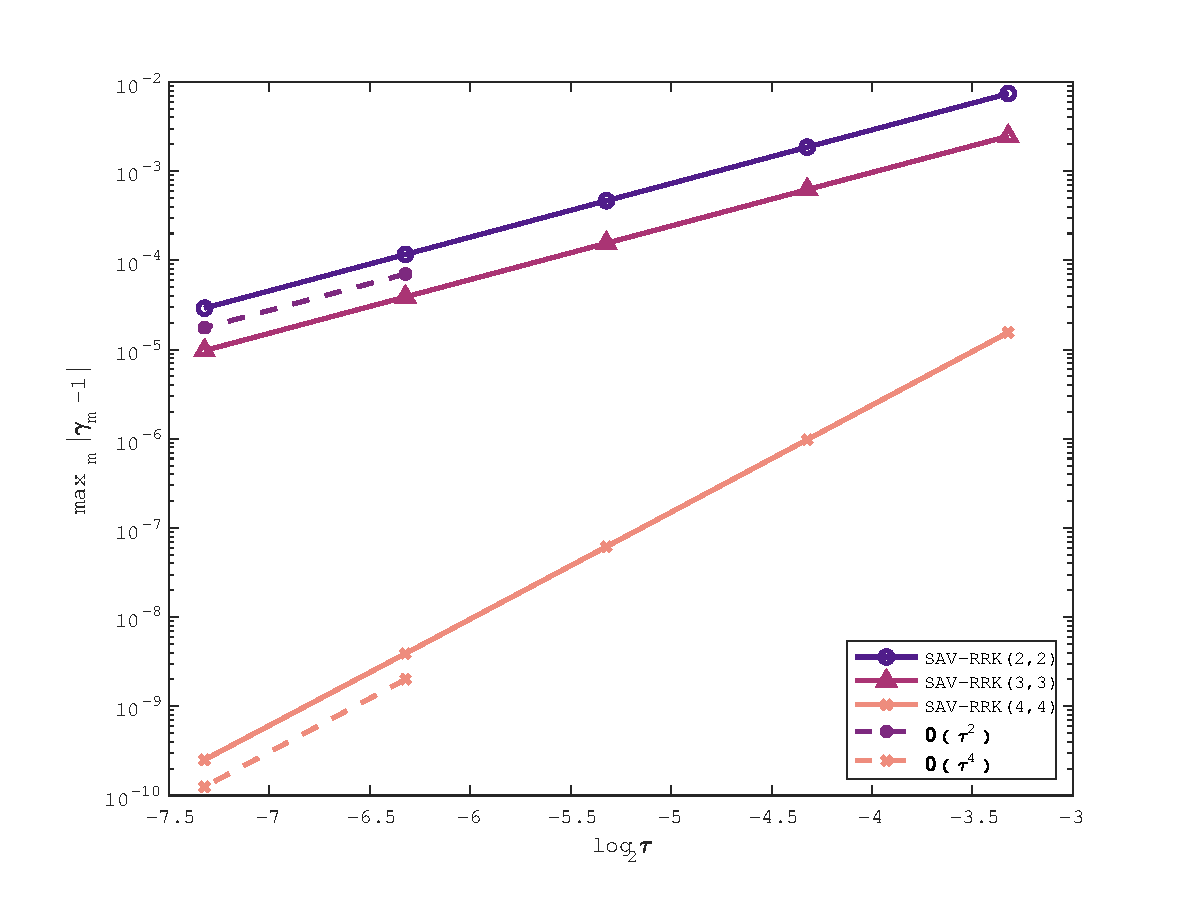
\includegraphics[width=0.5\textwidth]{./figures/exp1_r.eps}
		%\centerline{($b$) Spatial accuracy with $\tau = 10^{-3}.$}
		}\subfigure[$\max\limits_m\left|S_m(1)\right|$]{ \centering
		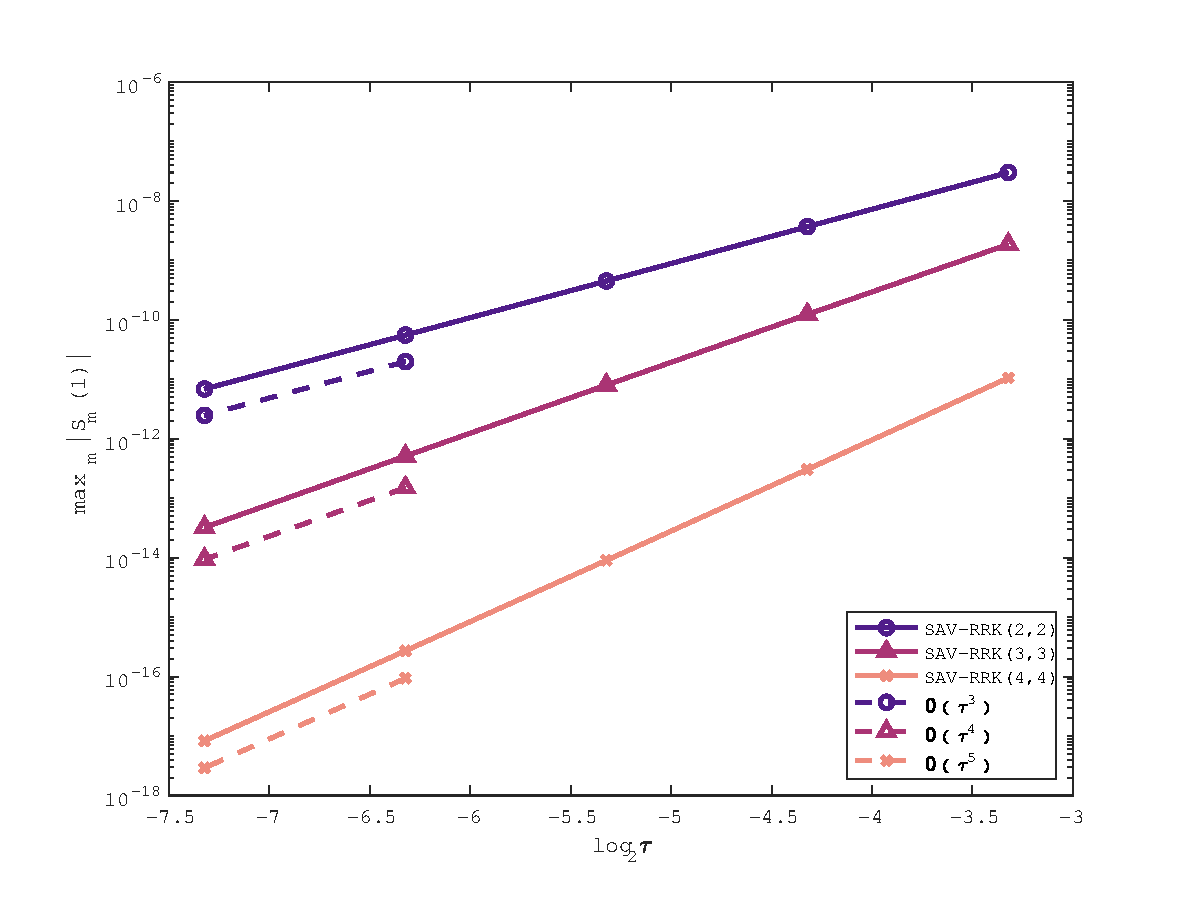
\includegraphics[width=0.5\textwidth]{./figures/exp1_s.eps}
		%\centerline{($a$) Temporal accuracy with $N=128.$}
		}\caption{$\max\limits_m\left|\gamma_m-1\right|$ and $\max\limits_m\left|S_m(1)\right|$ for some relaxation methods in Example \ref{exp_SAVRRK:1}.}
		\label{fig_SAVRRK:1}
		\end{center}
		\end{figure}
		我们还进行了一个长时间的模拟,直到 $T=1000$,并使用不同的 $\alpha$ 绘制了 SAV-RRK(4,4) 方法的相对能量图,如图 \ref{fig_SAVRRK:4} 所示。
		这表明所提出的方案可以在离散级别上完全保持能量,并且其保持性能明显优于 SAV 方法\cite{chengConvergenceEnergyconservingScheme2022} 和三级线性隐式差分法\cite{wangConservativeLinearizedDifference2015}。		

		\begin{figure}[H]
			\begin{center}
			\subfigure[$\alpha=1.3$]{ \centering
			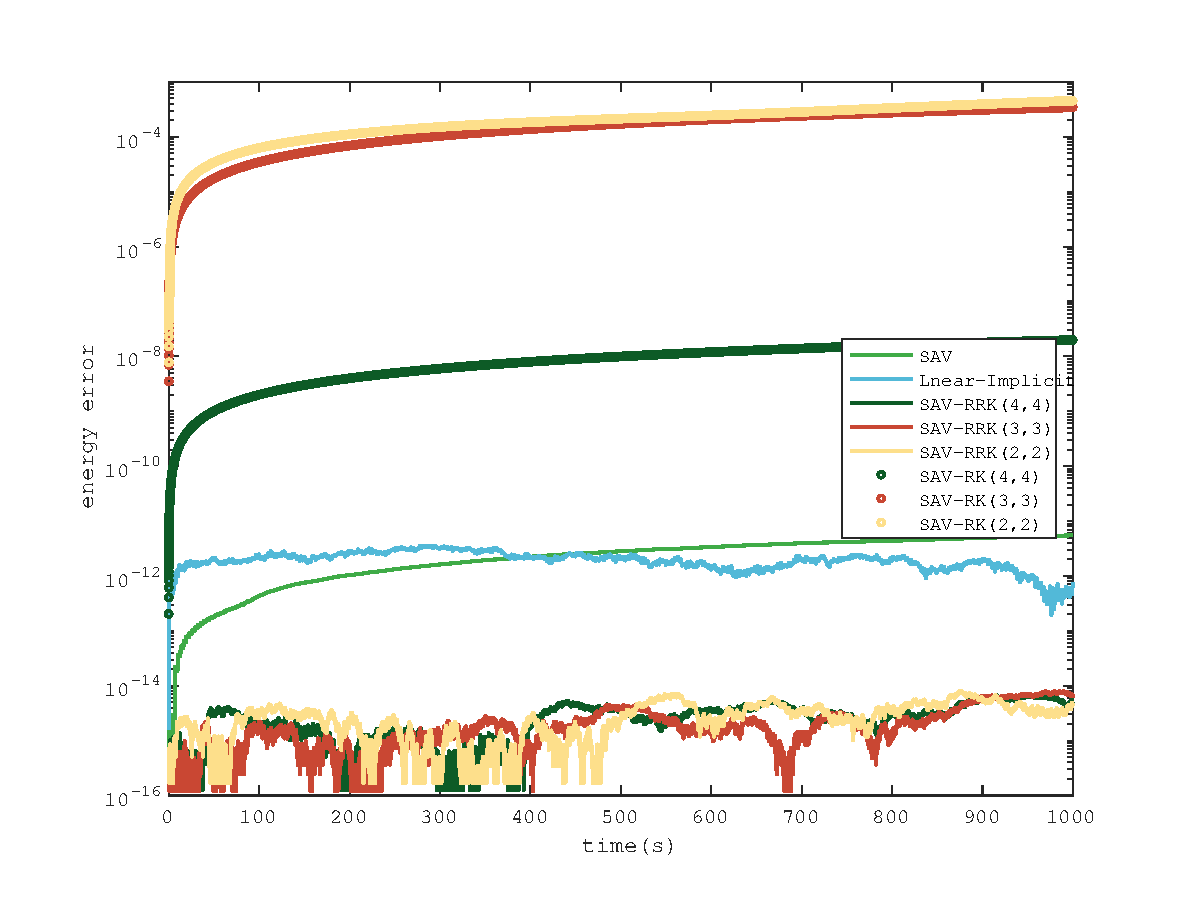
\includegraphics[width=0.5\textwidth]{./figures/exp1_energy3.eps}
			%\centerline{($b$) Spatial accuracy with $\tau = 10^{-3}.$}
			}\subfigure[$\alpha=1.6$]{ \centering
			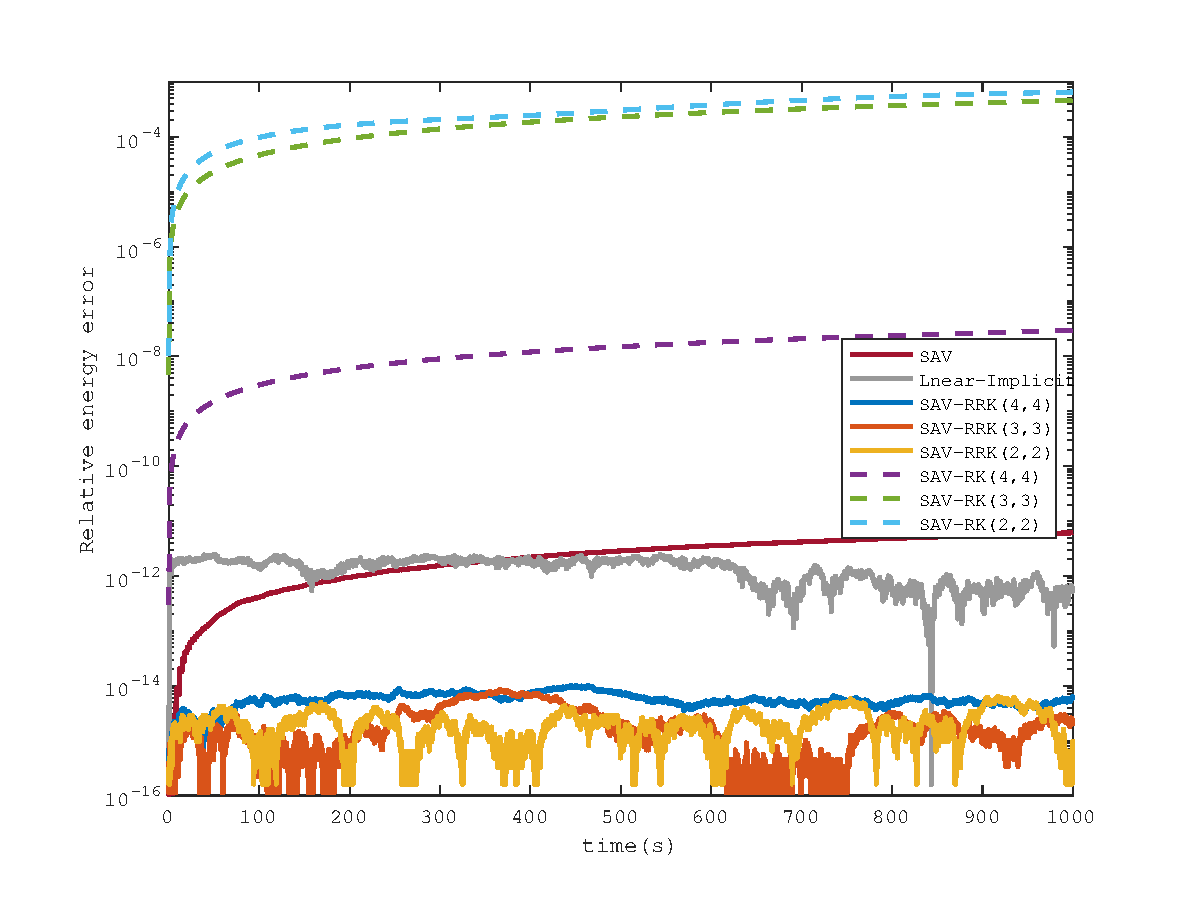
\includegraphics[width=0.5\textwidth]{./figures/exp1_energy6.eps}
			%\centerline{($a$) Temporal accuracy with $N=128.$}
			}\\
			\subfigure[$\alpha=1.9$]{ \centering
			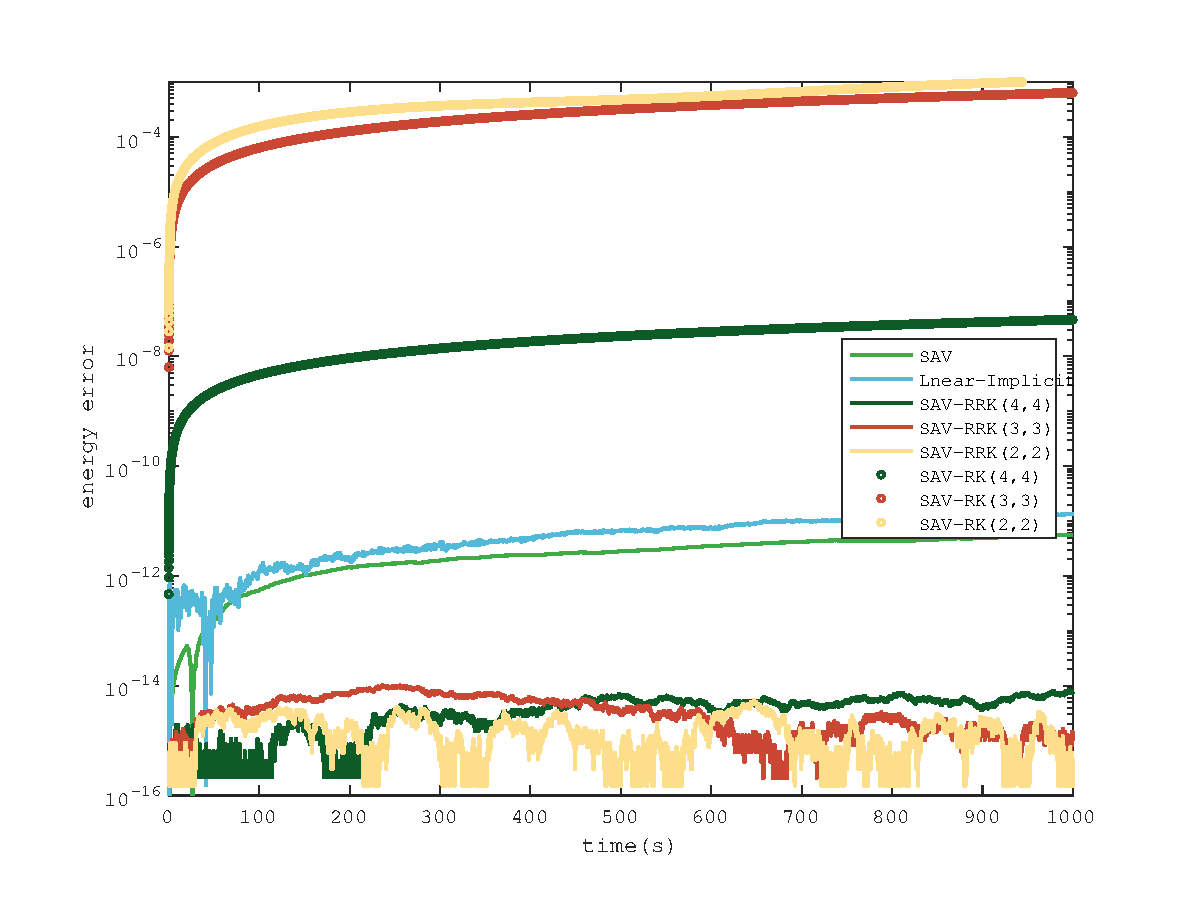
\includegraphics[width=0.5\textwidth]{./figures/exp1_energy9.eps}
			%\centerline{($b$) Spatial accuracy with $\tau = 10^{-3}.$}
			}\subfigure[$\alpha=2$]{ \centering
			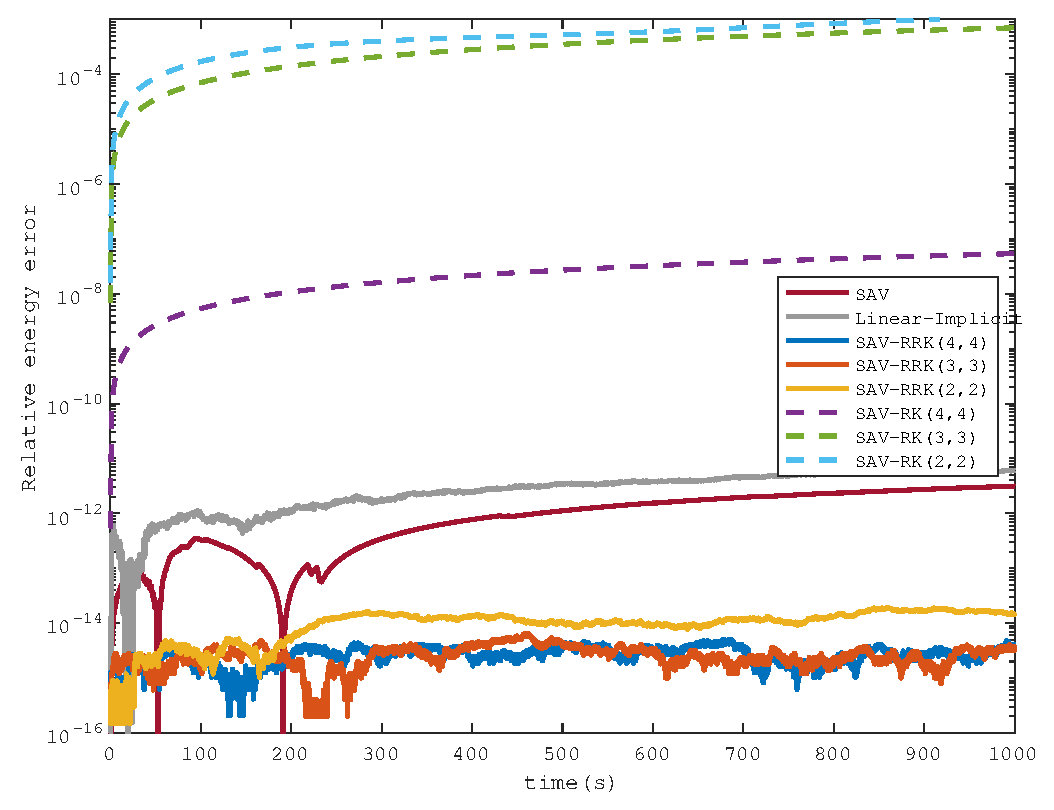
\includegraphics[width=0.5\textwidth]{./figures/exp1_energy2.eps}
			%\centerline{($a$) Temporal accuracy with $N=128.$}
			}\caption{ Relative errors of energy with $N=32, \tau=0.01$ for different $\alpha$ in Example \ref{exp_SAVRRK:1}.}
			\label{fig_SAVRRK:4}
			\end{center}
			\end{figure}

		\begin{example}\label{exp_SAVRRK:2}
			现在我们考虑具有以下初值的 2D NFSWEs \eqref{eq_SAVRRK:1}:
			\begin{equation*}
			u(x, y, 0)=\operatorname{sech}\left(x^2+y^2\right), u_t(x, y, 0)=\sin (x+y) \operatorname{sech}\left(-2\left(x^2+y^2\right)\right),(x, y, t) \in \Omega \times[0, T],
			\end{equation*}
			其中 $\Omega=[-5,5] \times[-5,5]$。
			\end{example}
				
				
			为了重新确认理论结果在 2D 情况下的适用性,
			考虑与例 \ref{exp_SAVRRK:1} 中相同的参数。也就是,$\alpha=1.5$ 和 $T=1$。
			表 \ref{tab_SAVRRK:6-2} 和图 \ref{fig_SAVRRK:2-1} 分别展示了时间上的收敛阶和弛豫系数 $\gamma$。
			我们可以观察到,与 1D 情况唯一的不同之处是,在 2D 情况下,SAV-RRK(IDT) 方法未能达到预期的更高阶。
	
\begin{table}[H]\footnotesize
	\centering
	\caption{Numerical errors and convergence order in time for Example \ref{exp_SAVRRK:2} when $N=4, T = 1$.}
	\begin{tabular}{lllllrlrlrlrlrl}
	\toprule
	\multicolumn{2}{l}{\multirow{2}[3]{*}{\textbf{RK(Stage,Order)}}} & \multicolumn{2}{l}{\multirow{2}[3]{*}{$\bm{\tau}$}} & \multicolumn{3}{c}{\textbf{SAV-RK}} &       & \multicolumn{3}{c}{\textbf{SAV-RRK}} &       & \multicolumn{3}{c}{\textbf{SAV-RRK(IDT)}} \\
	\cmidrule{5-7}\cmidrule{9-11}\cmidrule{13-15}    \multicolumn{2}{l}{} & \multicolumn{2}{l}{} & \textbf{Error($\tau$)} &       & \textbf{order} &       & \textbf{Error($\tau$)} &       & \textbf{order} &       & \textbf{Error($\tau$)} &       & \textbf{order} \\
	\hline
	\multicolumn{2}{l}{\multirow{5}[0]{*}{\textbf{RK(2,2)}}} & \multicolumn{2}{l}{0.1} & 3.0217E-03 &       & -     &       & 3.0102E-03 &       & -     &       & 1.5692E-02 &       & - \\
	\multicolumn{2}{l}{} & \multicolumn{2}{l}{0.05} & 7.4615E-04 &       & 2.0178  &       & 7.4702E-04 &       & 2.0106  &       & 9.6213E-03 &       & 0.7057  \\
	\multicolumn{2}{l}{} & \multicolumn{2}{l}{0.025} & 1.8513E-04 &       & 2.0109  &       & 1.8587E-04 &       & 2.0069  &       & 5.2472E-03 &       & 0.8747  \\
	\multicolumn{2}{l}{} & \multicolumn{2}{l}{0.0125} & 4.6090E-05 &       & 2.0060  &       & 4.6341E-05 &       & 2.0039  &       & 2.7312E-03 &       & 0.9420  \\
	\multicolumn{2}{l}{} & \multicolumn{2}{l}{0.00625} & 1.1497E-05 &       & 2.0032  &       & 1.1569E-05 &       & 2.0021  &       & 1.3923E-03 &       & 0.9721  \\
	\multicolumn{2}{l}{\multirow{5}[0]{*}{\textbf{RK(3,3)}}} & \multicolumn{2}{l}{0.1} & 1.2581E-04 &       & -     &       & 3.9379E-05 &       & -     &       & 3.2535E-03 &       & - \\
	\multicolumn{2}{l}{} & \multicolumn{2}{l}{0.05} & 1.6180E-05 &       & 2.9589  &       & 5.5726E-06 &       & 2.8210  &       & 7.9304E-04 &       & 2.0365  \\
	\multicolumn{2}{l}{} & \multicolumn{2}{l}{0.025} & 2.0532E-06 &       & 2.9783  &       & 7.4443E-07 &       & 2.9041  &       & 1.9546E-04 &       & 2.0205  \\
	\multicolumn{2}{l}{} & \multicolumn{2}{l}{0.0125} & 2.5863E-07 &       & 2.9889  &       & 9.6210E-08 &       & 2.9519  &       & 4.8500E-05 &       & 2.0108  \\
	\multicolumn{2}{l}{} & \multicolumn{2}{l}{0.00625} & 3.2454E-08 &       & 2.9944  &       & 1.2228E-08 &       & 2.9760  &       & 1.2078E-05 &       & 2.0056  \\
	\multicolumn{2}{l}{\multirow{5}[1]{*}{\textbf{RK(4,4)}}} & \multicolumn{2}{l}{0.1} & 7.9185E-06 &       & -     &       & 8.0508E-06 &       & -     &       & 3.4013E-05 &       & - \\
	\multicolumn{2}{l}{} & \multicolumn{2}{l}{0.05} & 4.9103E-07 &       & 4.0113  &       & 4.9644E-07 &       & 4.0194  &       & 3.3898E-06 &       & 3.3268  \\
	\multicolumn{2}{l}{} & \multicolumn{2}{l}{0.025} & 3.0531E-08 &       & 4.0075  &       & 3.0805E-08 &       & 4.0104  &       & 3.6901E-07 &       & 3.1995  \\
	\multicolumn{2}{l}{} & \multicolumn{2}{l}{0.0125} & 1.9026E-09 &       & 4.0042  &       & 1.9182E-09 &       & 4.0054  &       & 4.2681E-08 &       & 3.1120  \\
	\multicolumn{2}{l}{} & \multicolumn{2}{l}{0.00625} & 1.1873E-10 &       & 4.0022  &       & 1.1966E-10 &       & 4.0027  &       & 5.1191E-09 &       & 3.0596  \\
	\bottomrule
	\end{tabular}%
	\label{tab_SAVRRK:6-2}%
	\end{table}%
		
	\begin{figure}[H]
	\begin{center}
	\subfigure[$\max _m\left|\gamma_m-1\right|$]{ \centering
	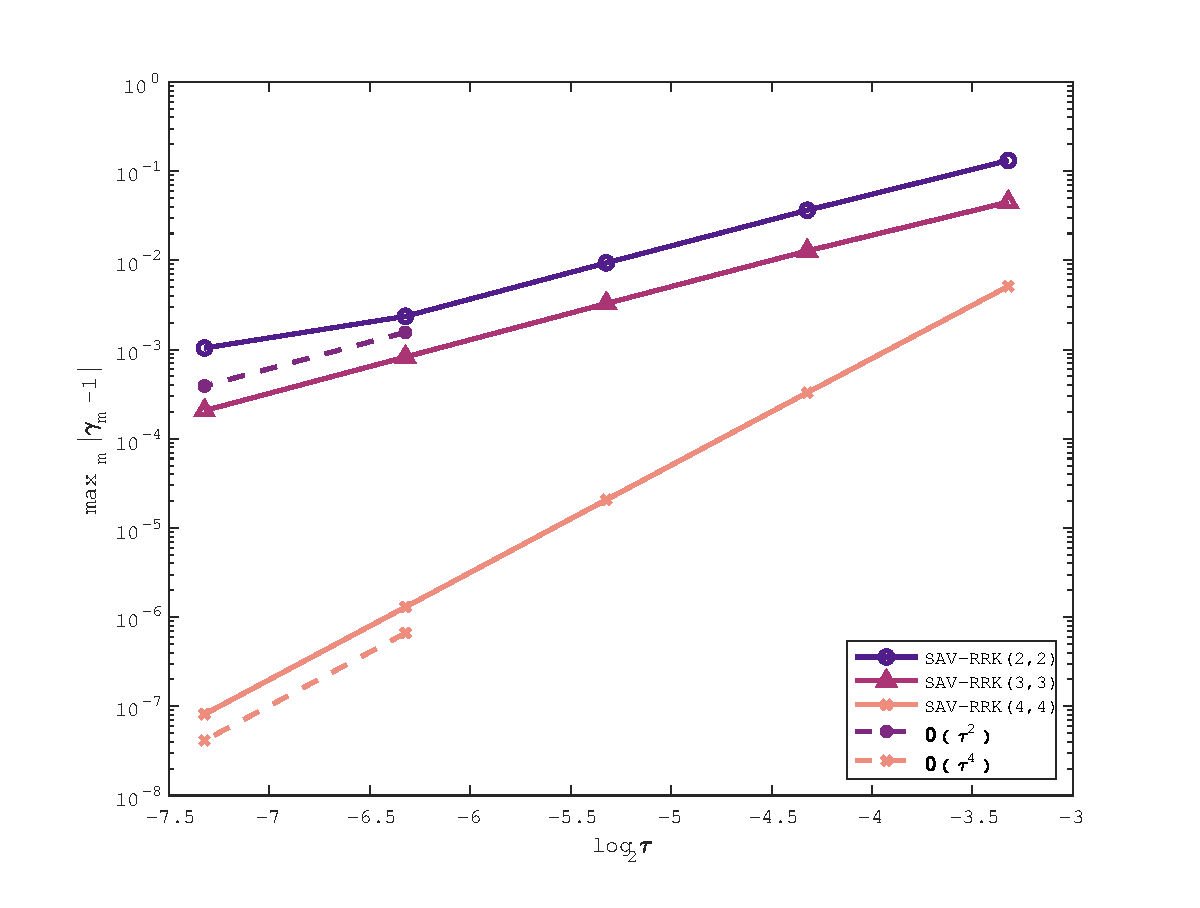
\includegraphics[width=0.5\textwidth]{./figures/exp2_r.eps}
	%\centerline{($b$) Spatial accuracy with $\tau = 10^{-3}.$}
	}\subfigure[$\max_m\left|S_m(1)\right|$]{ \centering
	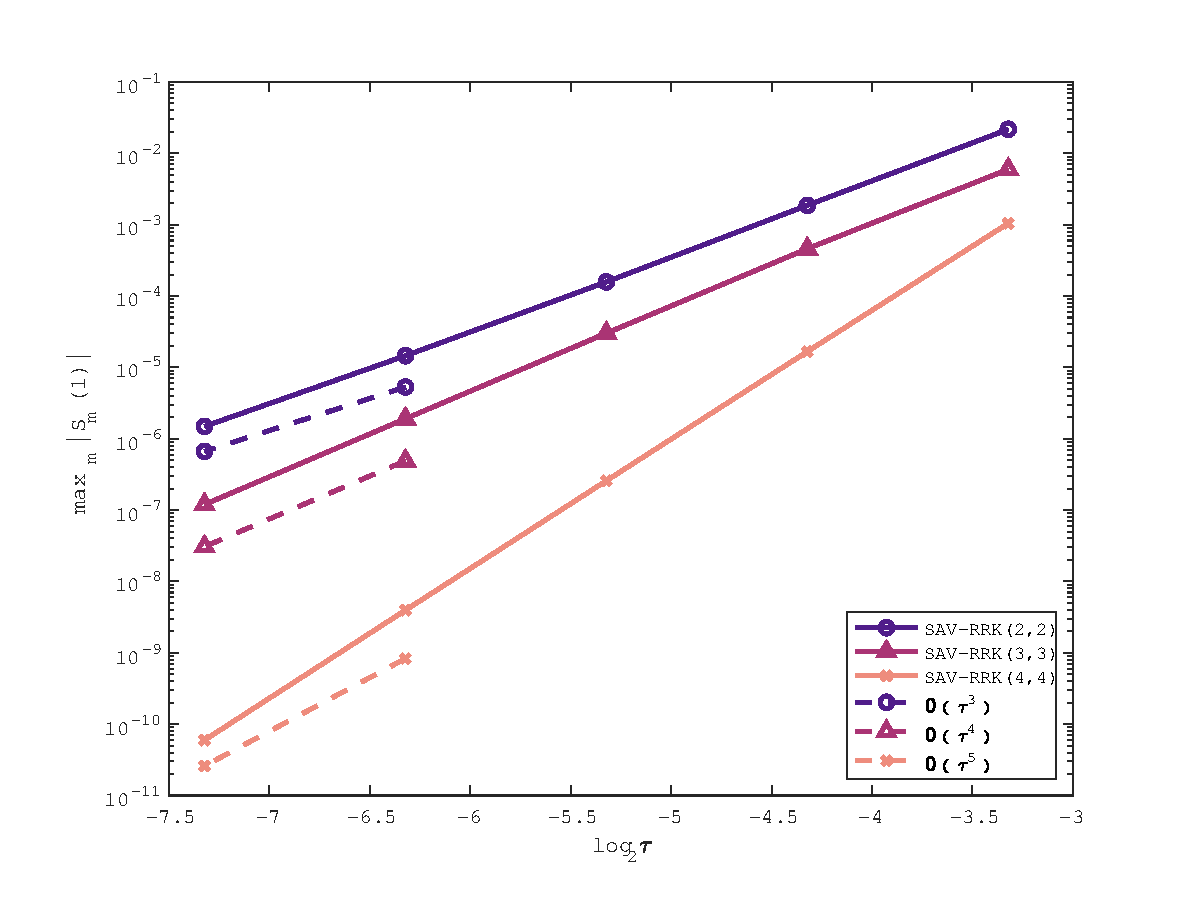
\includegraphics[width=0.5\textwidth]{./figures/exp2_s.eps}
	%\centerline{($a$) Temporal accuracy with $N=128.$}
	}\caption{$\max _m\left|\gamma_m-1\right|$ and $\max_m\left|S_m(1)\right|$ for some relaxation (RT) methods in Example \ref{exp_SAVRRK:2}.}
	\label{fig_SAVRRK:2-1}
	\end{center}
	\end{figure}
	为了展示所提方法在保持能量方面的有效性,我们进行了长时间模拟,直到 $T=100$,并在图 \ref{fig_SAVRRK:2-4} 中使用不同 $\alpha$ 的 SAV-RRK(4,4) 方法绘制了相对能量误差。结果显示,所提出的方法可以在离散级别上精确地保持能量,且其能量守恒性能显著优于文献 \cite{chengConvergenceEnergyconservingScheme2022} 中的 SAV 方法。
	\begin{figure}[H]
		\begin{center}
		\subfigure[$\alpha=1.3$]{ \centering
		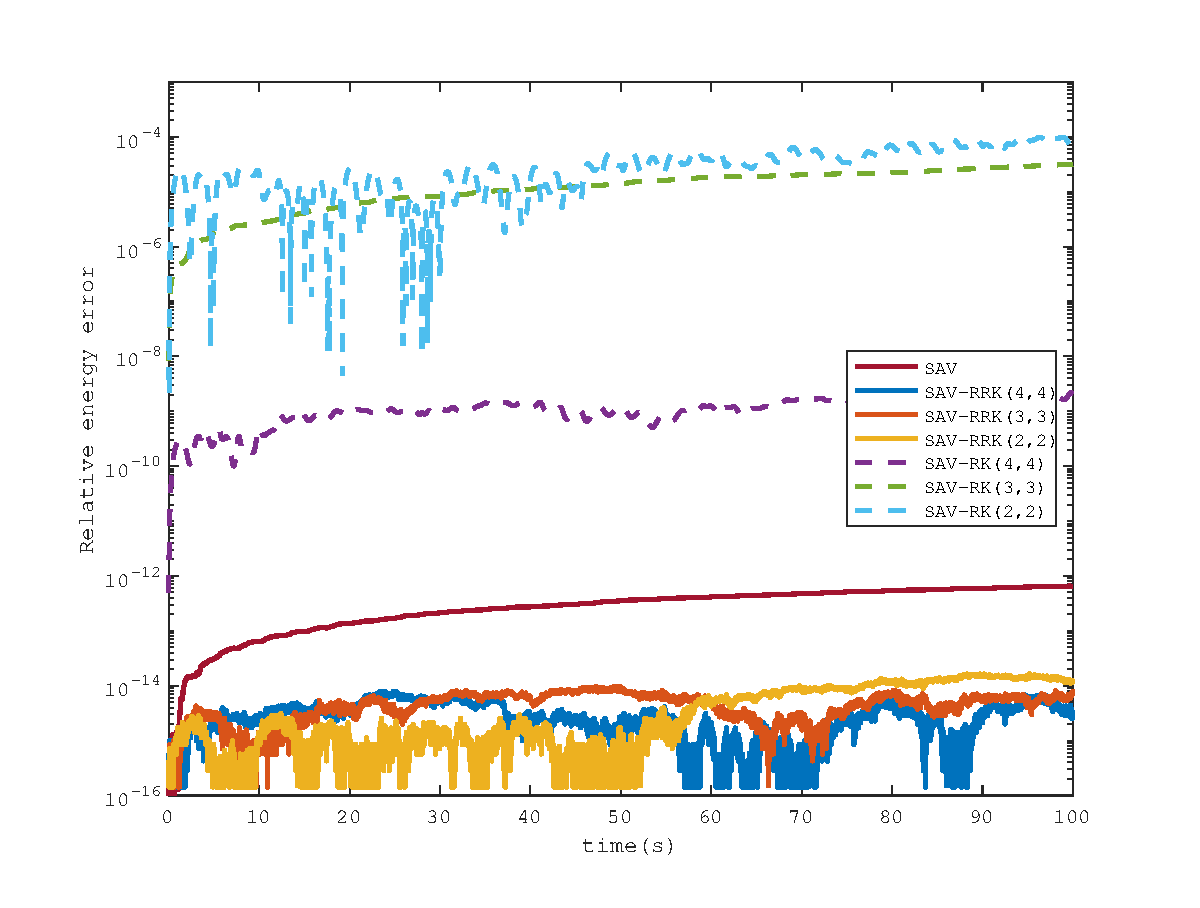
\includegraphics[width=0.5\textwidth]{./figures/exp2_energy3.eps}
		%\centerline{($b$) Spatial accuracy with $\tau = 10^{-3}.$}
		}\subfigure[$\alpha=1.6$]{ \centering
		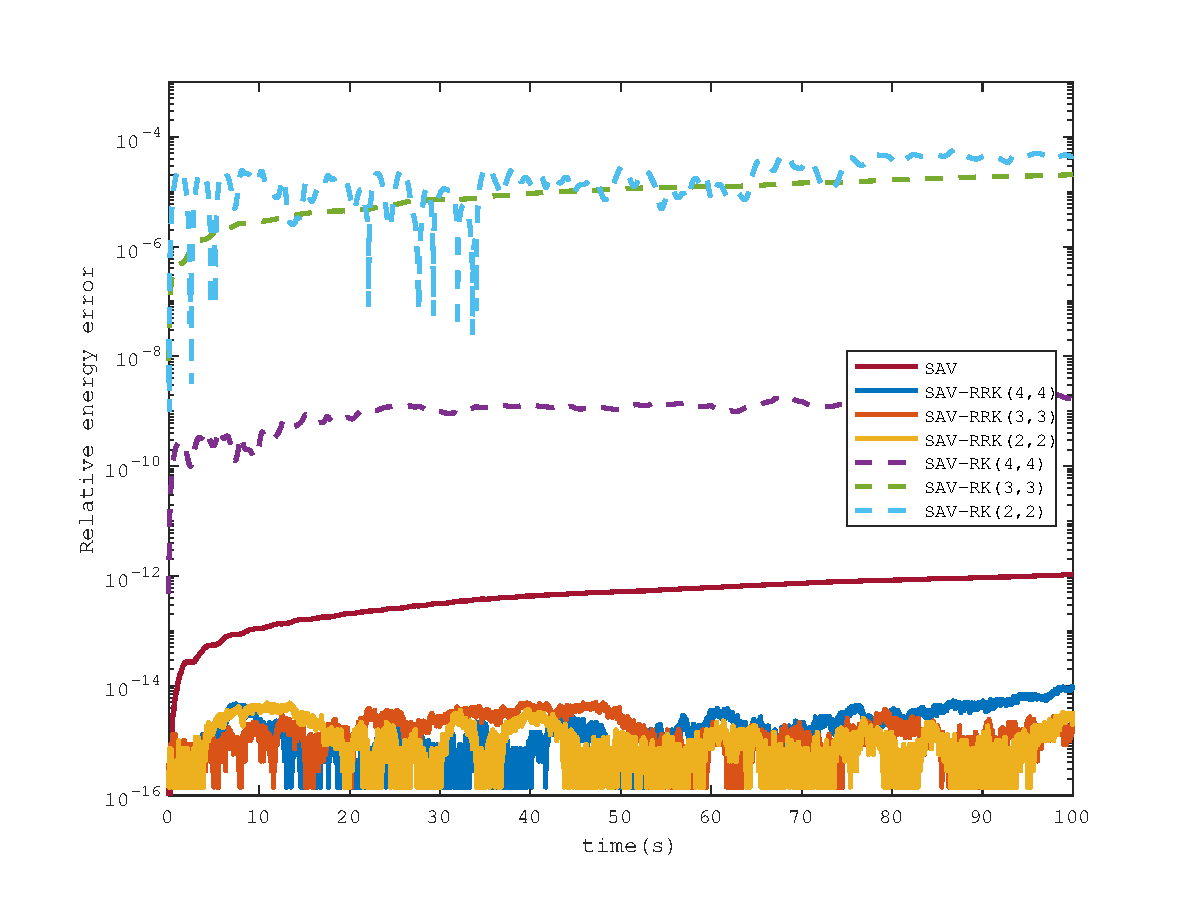
\includegraphics[width=0.5\textwidth]{./figures/exp2_energy6.eps}
		%\centerline{($a$) Temporal accuracy with $N=128.$}
		}\\
		\subfigure[$\alpha=1.9$]{ \centering
		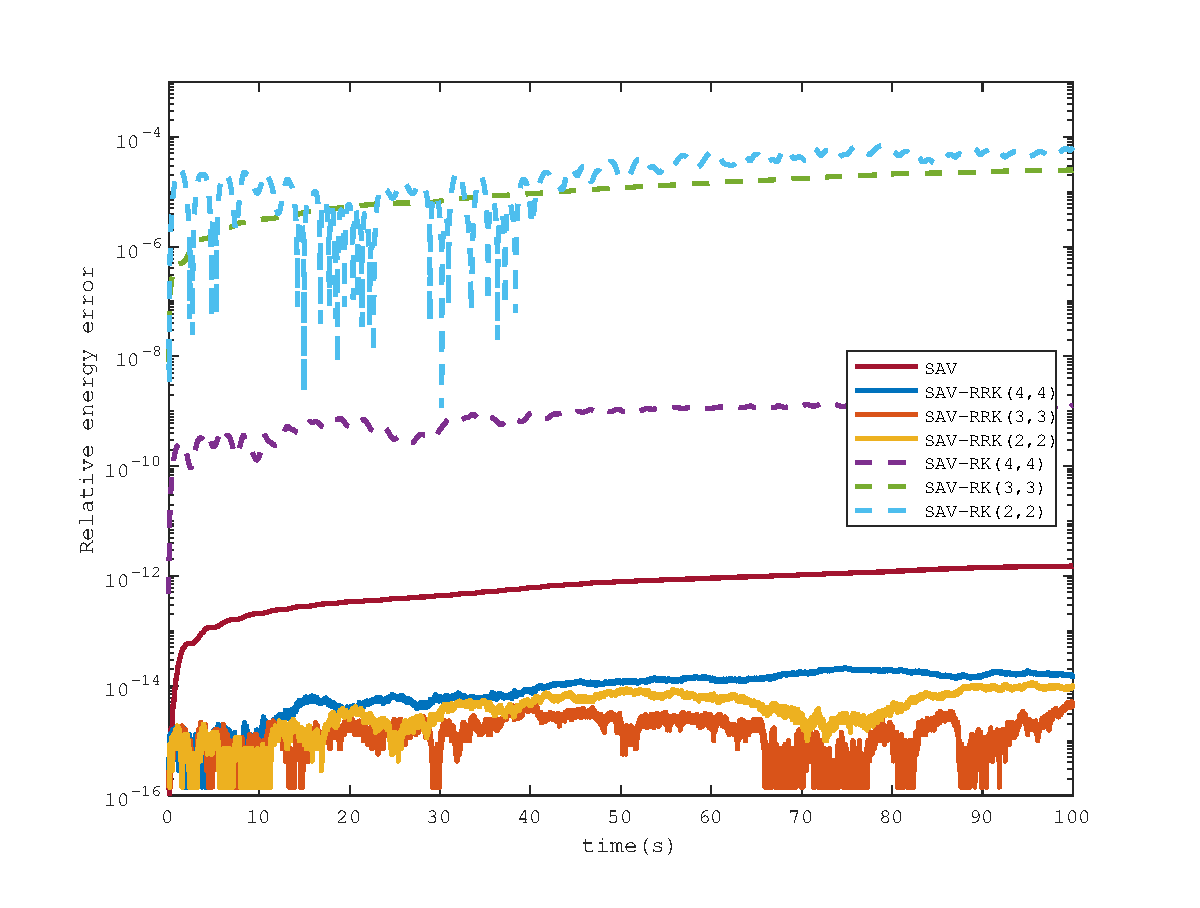
\includegraphics[width=0.5\textwidth]{./figures/exp2_energy9.eps}
		%\centerline{($b$) Spatial accuracy with $\tau = 10^{-3}.$}
		}\subfigure[$\alpha=2$]{ \centering
		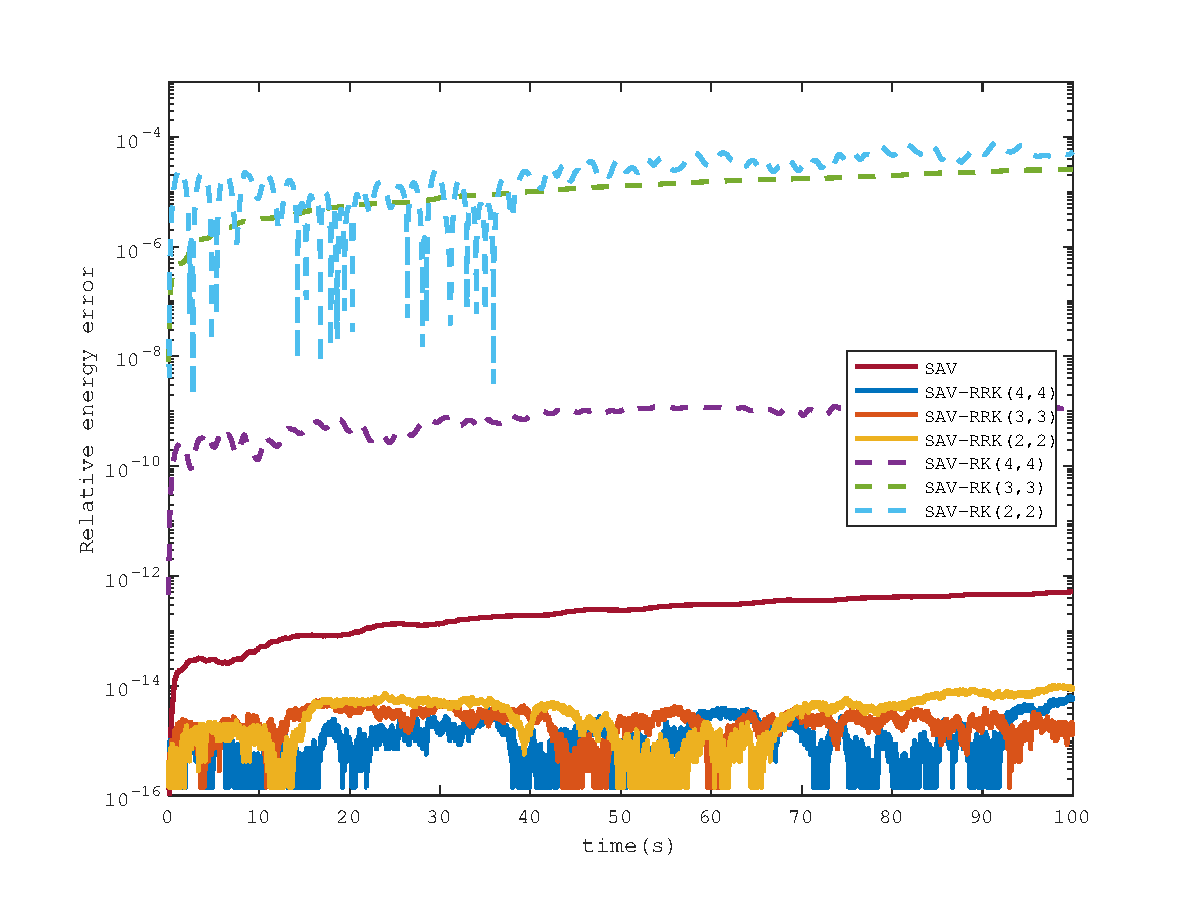
\includegraphics[width=0.5\textwidth]{./figures/exp2_energy2.eps}
		%\centerline{($a$) Temporal accuracy with $N=128.$}
		}\caption{ Relative errors of energy with $N=4, \tau=0.01$ for different $\alpha$ in Example \ref{exp_SAVRRK:2}.}
		\label{fig_SAVRRK:2-4}
		\end{center}
		\end{figure}
		
		\begin{example}\label{exp_SAVRRK:3}
			% \cite{wangUnconditionalEnergyDissipation2021} 
			接下来,我们考虑二维非线性分数阶波动方程
			\begin{equation}
			\begin{cases}
			& u_{t t}+(-\Delta)^{\frac{\alpha}{2}} u+F^{\prime}(u)=0,(x, y, t) \in \Omega \times(0, T],\\
			& u(x, y, 0)=\frac{1}{2} \arctan \left(\exp \left(-\sqrt{x^2+y^2}\right)\right), u_t(x, y, 0)=0,
			\end{cases}
			\end{equation}
			其中 $\Omega=(-10,10) \times(-10,10)$。
			\end{example}
			
			取势能 $F(u)=u^2\left(\frac{1}{4} u^2-\frac{1}{2}\right)$。在 $T=1$ 时,$\alpha=1.5$ 的时间收敛阶数如表 \ref{tab_SAVRRK:6-3} 所示。
			此外,图 \ref{fig_SAVRRK:3-4} 展示了长时间模拟 ($T=100$) 的离散能量演化,这些数据是通过应用 SAV-RRK(4,4) 方法计算的。结果表明,所提方法对非线性分数阶波动方程也是有效的。
			
\begin{table}[H]\footnotesize
\centering
\caption{Numerical errors and convergence order in time for Example \ref{exp_SAVRRK:3} when $N=4, T = 1$.}
\begin{tabular}{lllllrlrlrlrlrl}
\toprule
\multicolumn{2}{l}{\multirow{2}[3]{*}{\textbf{RK(Stage,Order)}}} & \multicolumn{2}{l}{\multirow{2}[3]{*}{$\bm{\tau}$}} & \multicolumn{3}{c}{\textbf{SAV-RK}} &       & \multicolumn{3}{c}{\textbf{SAV-RRK(RT)}} &       & \multicolumn{3}{c}{\textbf{SAV-RRK(IDT)}} \\
\cmidrule{5-7}\cmidrule{9-11}\cmidrule{13-15}    \multicolumn{2}{l}{} & \multicolumn{2}{l}{} & \textbf{Error($\tau$)} &       & \textbf{order} &       & \textbf{Error($\tau$)} &       & \textbf{order} &       & \textbf{Error($\tau$)} &       & \textbf{order} \\
\hline
\multicolumn{2}{l}{\multirow{5}[0]{*}{\textbf{RK(2,2)}}} & \multicolumn{2}{l}{0.1} & 1.3395E-03 &       & -     &       & 3.3870E-03 &       & -     &       & 2.1470E-02 &       & - \\
\multicolumn{2}{l}{} & \multicolumn{2}{l}{0.05} & 3.4360E-04 &       & 1.9628  &       & 8.1480E-04 &       & 2.0555  &       & 1.0960E-02 &       & 0.9701  \\
\multicolumn{2}{l}{} & \multicolumn{2}{l}{0.025} & 8.6945E-05 &       & 1.9826  &       & 1.9951E-04 &       & 2.0300  &       & 5.5113E-03 &       & 0.9918  \\
\multicolumn{2}{l}{} & \multicolumn{2}{l}{0.0125} & 2.1865E-05 &       & 1.9915  &       & 4.9347E-05 &       & 2.0154  &       & 2.7600E-03 &       & 0.9977  \\
\multicolumn{2}{l}{} & \multicolumn{2}{l}{0.00625} & 5.4823E-06 &       & 1.9958  &       & 1.2270E-05 &       & 2.0078  &       & 1.3807E-03 &       & 0.9993  \\
\multicolumn{2}{l}{\multirow{5}[0]{*}{\textbf{RK(3,3)}}} & \multicolumn{2}{l}{0.1} & 3.5168E-05 &       & -     &       & 4.3927E-05 &       & -     &       & 3.8213E-04 &       & - \\
\multicolumn{2}{l}{} & \multicolumn{2}{l}{0.05} & 4.3533E-06 &       & 3.0141  &       & 5.4825E-06 &       & 3.0022  &       & 8.0473E-05 &       & 2.2475  \\
\multicolumn{2}{l}{} & \multicolumn{2}{l}{0.025} & 5.3902E-07 &       & 3.0137  &       & 6.8378E-07 &       & 3.0032  &       & 1.8560E-05 &       & 2.1163  \\
\multicolumn{2}{l}{} & \multicolumn{2}{l}{0.0125} & 6.7058E-08 &       & 3.0068  &       & 8.5344E-08 &       & 3.0022  &       & 4.4475E-06 &       & 2.0611  \\
\multicolumn{2}{l}{} & \multicolumn{2}{l}{0.00625} & 8.3615E-09 &       & 3.0036  &       & 1.0659E-08 &       & 3.0012  &       & 1.0883E-06 &       & 2.0309  \\
\multicolumn{2}{l}{\multirow{5}[1]{*}{\textbf{RK(4,4)}}} & \multicolumn{2}{l}{0.1} & 5.3561E-07 &       & -     &       & 3.2716E-06 &       & -     &       & 3.7745E-05 &       & - \\
\multicolumn{2}{l}{} & \multicolumn{2}{l}{0.05} & 3.6438E-08 &       & 3.8777  &       & 2.0654E-07 &       & 3.9855  &       & 4.8050E-06 &       & 2.9737  \\
\multicolumn{2}{l}{} & \multicolumn{2}{l}{0.025} & 2.3735E-09 &       & 3.9403  &       & 1.2898E-08 &       & 4.0012  &       & 6.0237E-07 &       & 2.9958  \\
\multicolumn{2}{l}{} & \multicolumn{2}{l}{0.0125} & 1.5146E-10 &       & 3.9700  &       & 8.0476E-10 &       & 4.0024  &       & 7.5303E-08 &       & 2.9999  \\
\multicolumn{2}{l}{} & \multicolumn{2}{l}{0.00625} & 9.5636E-12 &       & 3.9853  &       & 5.0241E-11 &       & 4.0016  &       & 9.4105E-09 &       & 3.0004  \\
\bottomrule
\end{tabular}%
\label{tab_SAVRRK:6-3}%
\end{table}%
\vspace{-10mm}

\begin{figure}[H]
\begin{center}
\subfigure[$\alpha=1.3$]{ \centering
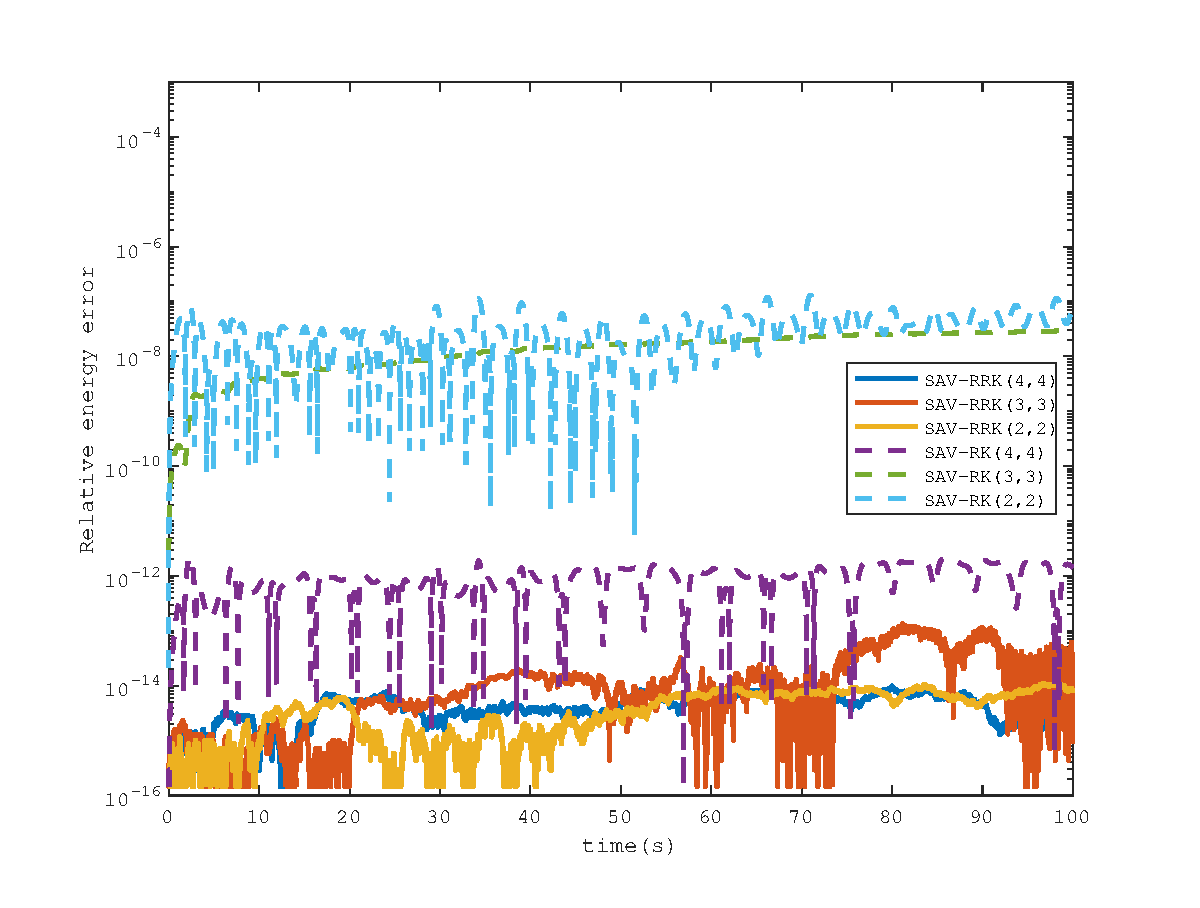
\includegraphics[width=0.5\textwidth]{./figures/exp3_energy3.eps}
%\centerline{($b$) Spatial accuracy with $\tau = 10^{-3}.$}
}\subfigure[$\alpha=1.6$]{ \centering
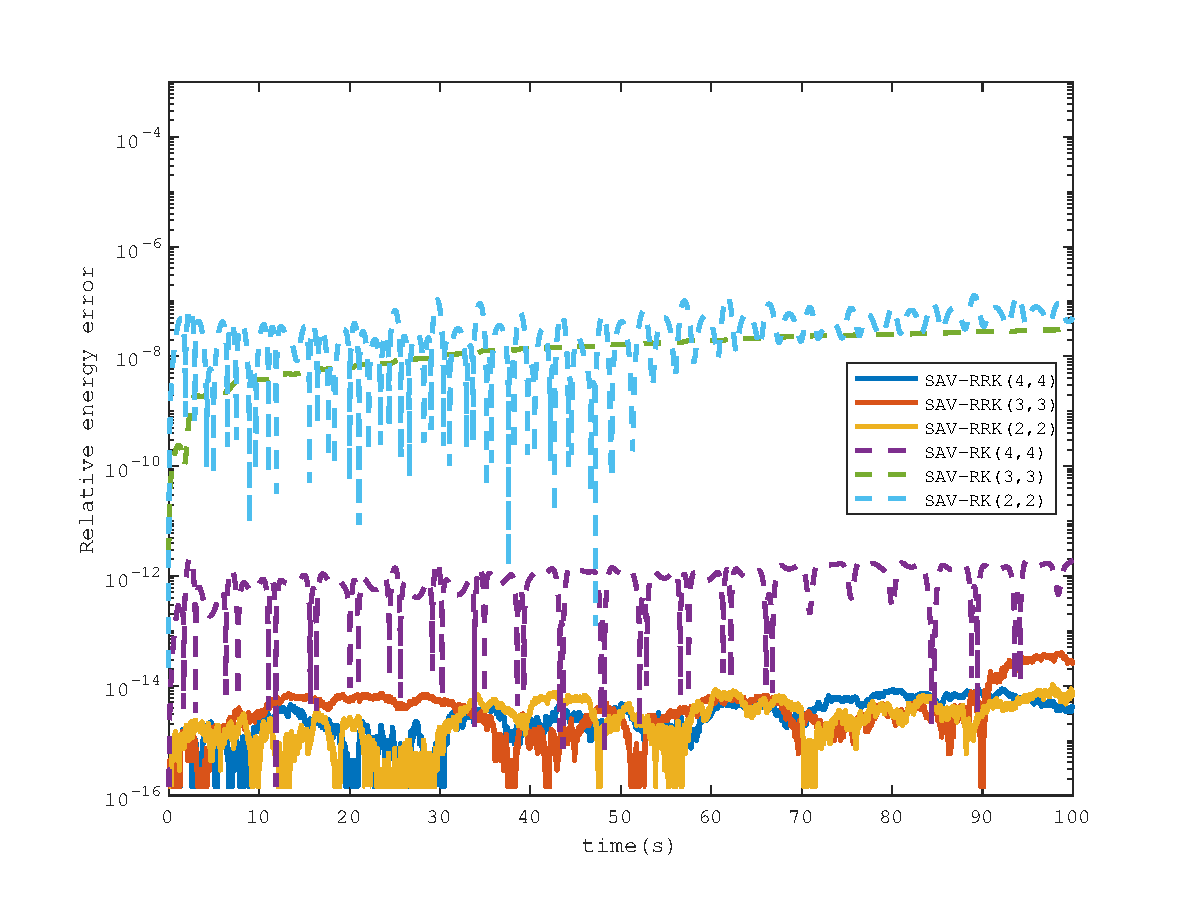
\includegraphics[width=0.5\textwidth]{./figures/exp3_energy6.eps}
%\centerline{($a$) Temporal accuracy with $N=128.$}
}\\
\subfigure[$\alpha=1.9$]{ \centering
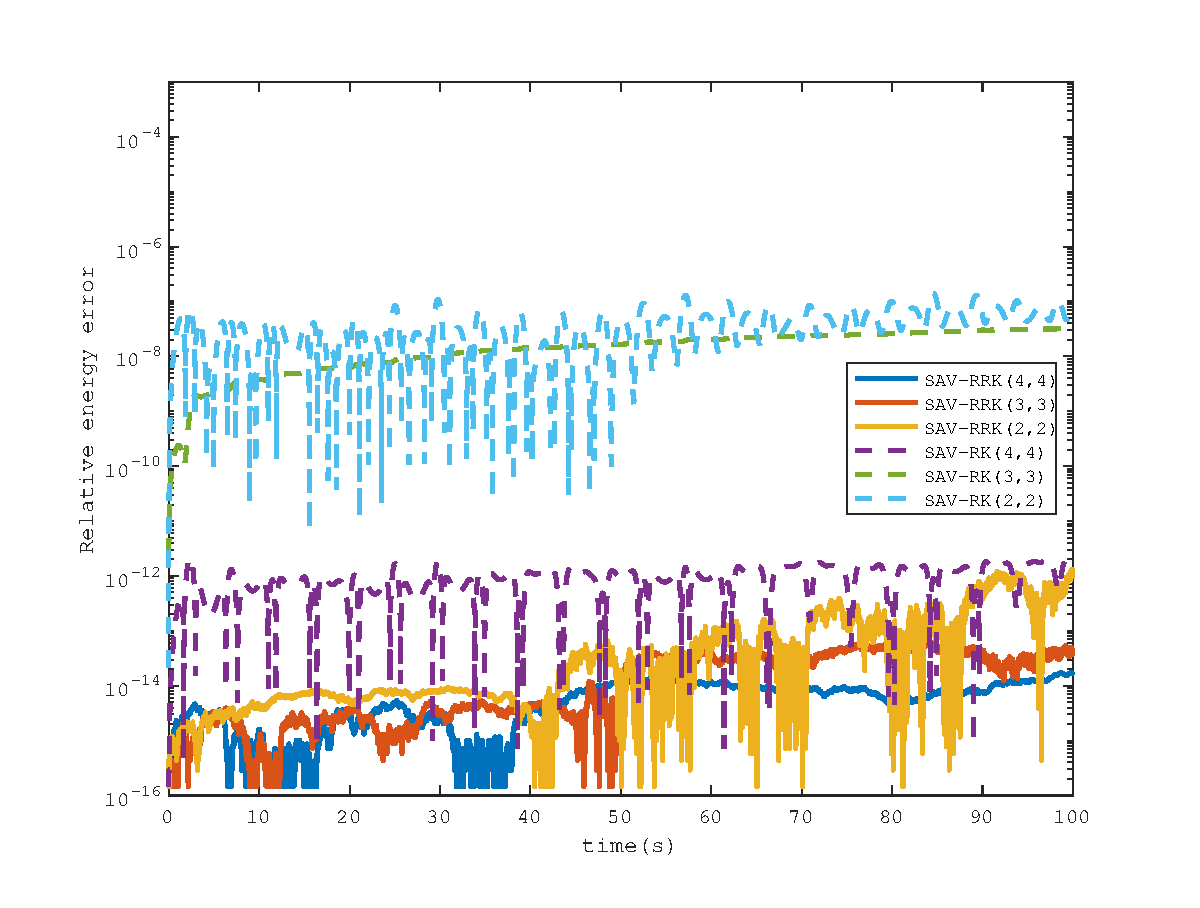
\includegraphics[width=0.5\textwidth]{./figures/exp3_energy9.eps}
%\centerline{($b$) Spatial accuracy with $\tau = 10^{-3}.$}
}\subfigure[$\alpha=2$]{ \centering
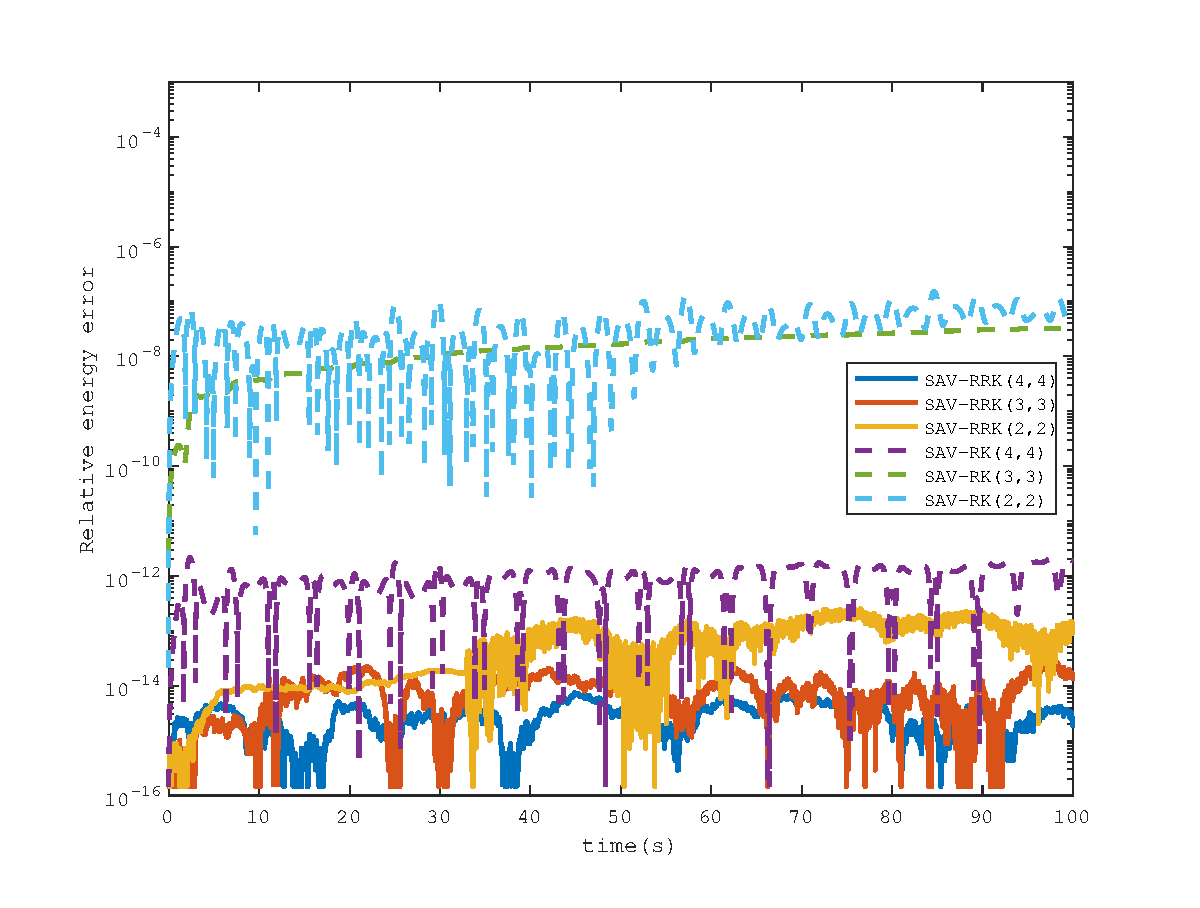
\includegraphics[width=0.5\textwidth]{./figures/exp3_energy2.eps}
%\centerline{($a$) Temporal accuracy with $N=128.$}
}\caption{ Relative errors of energy with $N=4, \tau=0.01$ for different $\alpha$ in Example \ref{exp_SAVRRK:3}.}
\label{fig_SAVRRK:3-4}
\end{center}
\end{figure}

\begin{example}\label{exp_SAVRRK:4}
	% \cite{fuStructurepreservingAlgorithmsTwodimensional2020} 
	最后,我们考虑二维分数阶Klein-Gordon-Schr{\"o}dinger方程
	\begin{equation}
	\begin{cases}
	\mathrm{i} \partial_t u-\frac{1}{2}(-\Delta)^{\frac{\alpha}{2}} u+u \phi=0,(x, y, t) \in \Omega \times(0, T],\\
	\partial_{t t} \phi+(-\Delta)^{\frac{\beta}{2}} \phi+\phi-|u|^2=0, (x, y, t) \in \Omega \times(0, T],
	\end{cases}
	\end{equation}
	其中初始条件为
	\begin{equation}
	u(x, y, 0)=(1+\mathrm{i}) \exp \left(-|\boldsymbol{x}|^2\right),~~\phi(x, y, 0)=\operatorname{sech}\left(|\boldsymbol{x}|^2\right),~~ \partial_t \phi(x, y, 0)=\sin (x+y) \operatorname{sech}\left(-2|\boldsymbol{x}|^2\right),
	\end{equation}
	其中 $\Omega=[-10,10] \times[-10,10]$。
	\end{example}
	
	与前面的例子类似,表 \ref{tab_SAVRRK:6-4} 列出了 $\alpha=\beta=1.5$ 时的一些数值误差和时间收敛阶数。

	
\begin{table}[H]\footnotesize
	\centering
	\caption{Numerical errors and convergence order in time for Example \ref{exp_SAVRRK:4} when $N=4, T = 1$.}
	\begin{tabular}{lllllrlrlrlrlrl}
	\toprule
	\multicolumn{2}{l}{\multirow{2}[3]{*}{\textbf{RK(Stage,Order)}}} & \multicolumn{2}{l}{\multirow{2}[3]{*}{$\bm{\tau}$}} & \multicolumn{3}{c}{\textbf{SAV-RK}} &       & \multicolumn{3}{c}{\textbf{SAV-RRK(RT)}} &       & \multicolumn{3}{c}{\textbf{SAV-RRK(IDT)}} \\
	\cmidrule{5-7}\cmidrule{9-11}\cmidrule{13-15}    \multicolumn{2}{l}{} & \multicolumn{2}{l}{} & \textbf{Error($\tau$)} &       & \textbf{order} &       & \textbf{Error($\tau$)} &       & \textbf{order} &       & \textbf{Error($\tau$)} &       & \textbf{order} \\
	\hline
	\multicolumn{2}{l}{\multirow{5}[0]{*}{\textbf{RK(2,2)}}} & \multicolumn{2}{l}{0.1} & 1.1875E-03 &       & -     &       & 1.8837E-03 &       & -     &       & 9.5325E-03 &       & - \\
	\multicolumn{2}{l}{} & \multicolumn{2}{l}{0.05} & 2.7648E-04 &       & 2.1026  &       & 5.0394E-04 &       & 1.9023  &       & 6.7134E-03 &       & 0.5058  \\
	\multicolumn{2}{l}{} & \multicolumn{2}{l}{0.025} & 6.6514E-05 &       & 2.0555  &       & 1.3036E-04 &       & 1.9508  &       & 3.8805E-03 &       & 0.7908  \\
	\multicolumn{2}{l}{} & \multicolumn{2}{l}{0.0125} & 1.6300E-05 &       & 2.0288  &       & 3.3151E-05 &       & 1.9754  &       & 2.0757E-03 &       & 0.9026  \\
	\multicolumn{2}{l}{} & \multicolumn{2}{l}{0.00625} & 4.0339E-06 &       & 2.0146  &       & 8.3587E-06 &       & 1.9877  &       & 1.0723E-03 &       & 0.9529  \\
	\multicolumn{2}{l}{\multirow{5}[0]{*}{\textbf{RK(3,3)}}} & \multicolumn{2}{l}{0.1} & 8.7748E-05 &       & -     &       & 1.9567E-04 &       & -     &       & 3.1789E-03 &       & - \\
	\multicolumn{2}{l}{} & \multicolumn{2}{l}{0.05} & 1.1471E-05 &       & 2.9354  &       & 2.4630E-05 &       & 2.9900  &       & 8.2646E-04 &       & 1.9435  \\
	\multicolumn{2}{l}{} & \multicolumn{2}{l}{0.025} & 1.4684E-06 &       & 2.9657  &       & 3.0916E-06 &       & 2.9940  &       & 2.1079E-04 &       & 1.9712  \\
	\multicolumn{2}{l}{} & \multicolumn{2}{l}{0.0125} & 1.8580E-07 &       & 2.9824  &       & 3.8731E-07 &       & 2.9968  &       & 5.3231E-05 &       & 1.9854  \\
	\multicolumn{2}{l}{} & \multicolumn{2}{l}{0.00625} & 2.3370E-08 &       & 2.9911  &       & 4.8471E-08 &       & 2.9983  &       & 1.3375E-05 &       & 1.9927  \\
	\multicolumn{2}{l}{\multirow{5}[1]{*}{\textbf{RK(4,4)}}} & \multicolumn{2}{l}{0.1} & 3.0741E-06 &       & -     &       & 4.0627E-06 &       & -     &       & 1.0278E-04 &       & - \\
	\multicolumn{2}{l}{} & \multicolumn{2}{l}{0.05} & 1.9959E-07 &       & 3.9450  &       & 2.6020E-07 &       & 3.9647  &       & 1.3195E-05 &       & 2.9615  \\
	\multicolumn{2}{l}{} & \multicolumn{2}{l}{0.025} & 1.2698E-08 &       & 3.9744  &       & 1.6461E-08 &       & 3.9825  &       & 1.6711E-06 &       & 2.9811  \\
	\multicolumn{2}{l}{} & \multicolumn{2}{l}{0.0125} & 8.0044E-10 &       & 3.9876  &       & 1.0350E-09 &       & 3.9913  &       & 2.1024E-07 &       & 2.9906  \\
	\multicolumn{2}{l}{} & \multicolumn{2}{l}{0.00625} & 5.0238E-11 &       & 3.9939  &       & 6.4882E-11 &       & 3.9957  &       & 2.6365E-08 &       & 2.9953  \\
	\bottomrule
	\end{tabular}%
	\label{tab_SAVRRK:6-4}%
	\end{table}%

	此外,长时间模拟(直至 $T=100$)中使用不同 $\alpha$ 和 $\beta$ 的相对能量如图 \ref{fig_SAVRRK:3-5} 所示。
% 图像展示的现象表明,所提出的方案可以在分数阶Klein-Gordon-Schr{\"o}dinger方程的离散水平上准确保持能量。
图中所示的现象表明,所提出的方法可以在分数阶Klein-Gordon-Schr{\"o}dinger方程的离散水平上准确保持能量。

\begin{figure}[H]
	\begin{center}
	\subfigure[$\alpha,\beta=1.3$]{ \centering
	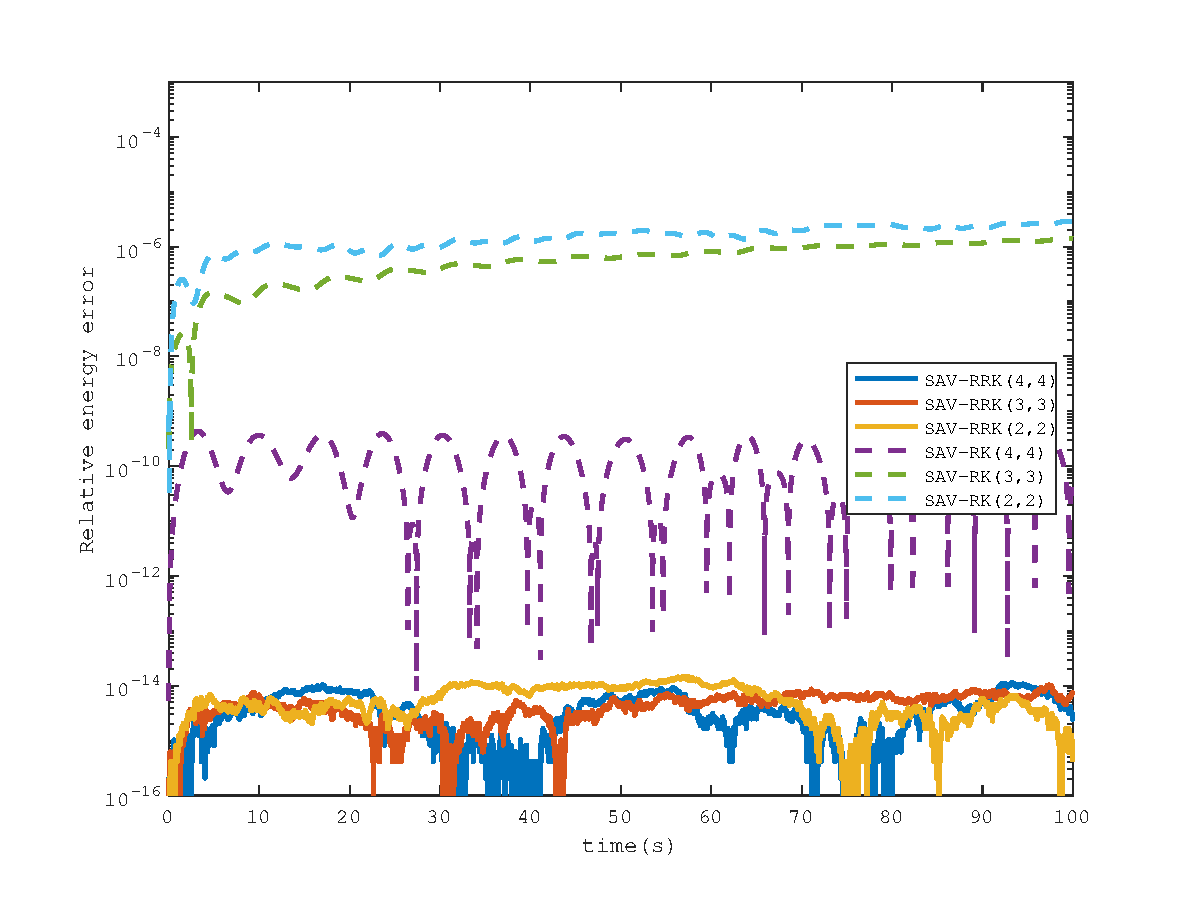
\includegraphics[width=0.5\textwidth]{./figures/exp4_energy3.eps}
	%\centerline{($b$) Spatial accuracy with $\tau = 10^{-3}.$}
	}\subfigure[$\alpha,\beta=1.6$]{ \centering
	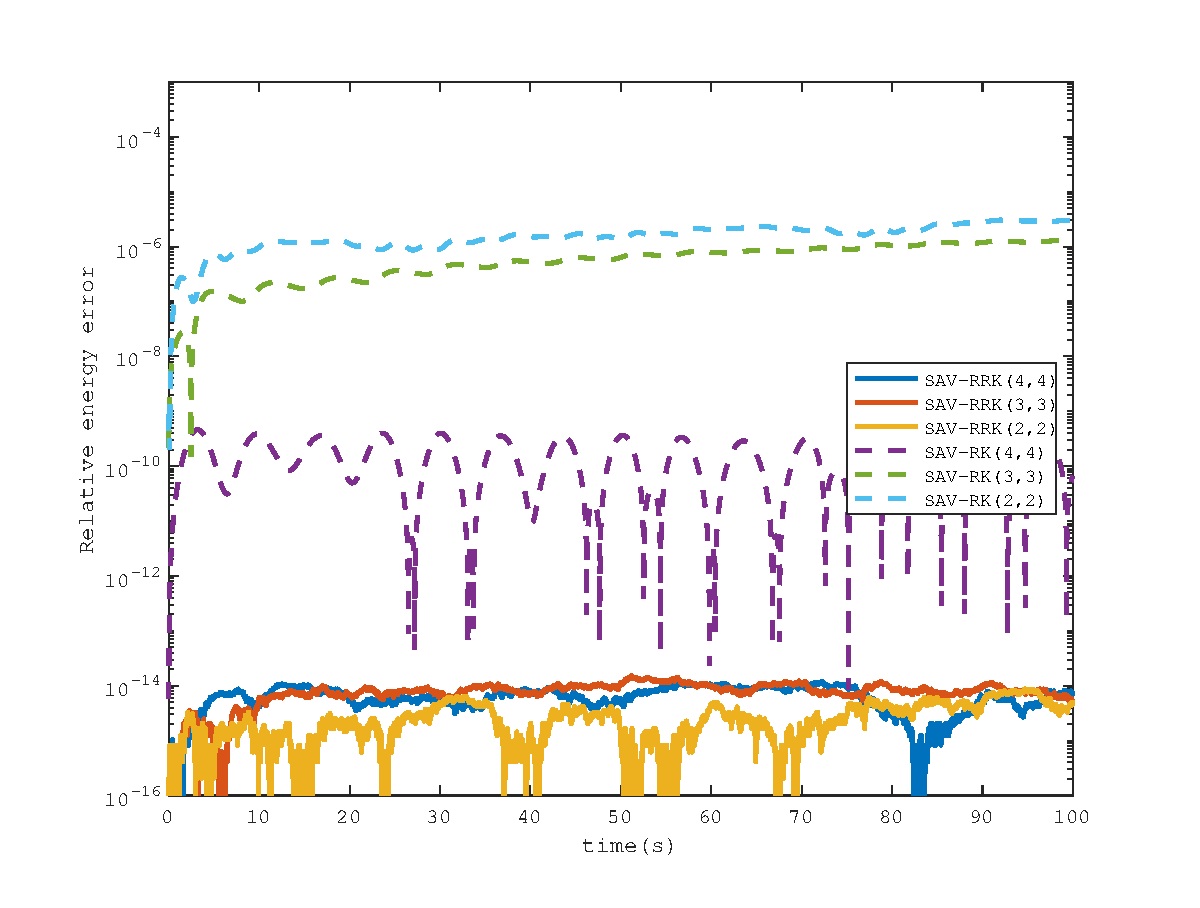
\includegraphics[width=0.5\textwidth]{./figures/exp4_energy6.eps}
	%\centerline{($a$) Temporal accuracy with $N=128.$}
	}\\
	\subfigure[$\alpha,\beta=1.9$]{ \centering
	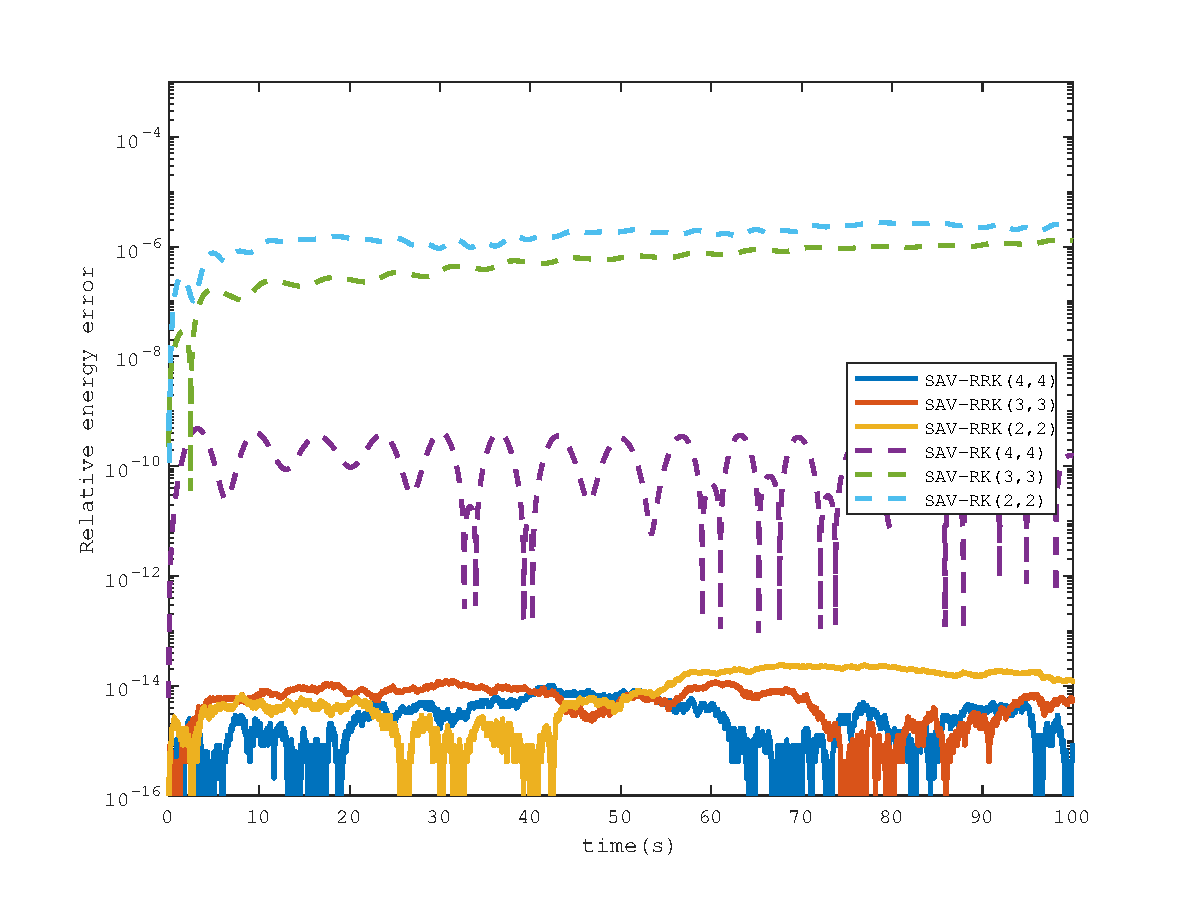
\includegraphics[width=0.5\textwidth]{./figures/exp4_energy9.eps}
	%\centerline{($b$) Spatial accuracy with $\tau = 10^{-3}.$}
	}\subfigure[$\alpha,\beta=2$]{ \centering
	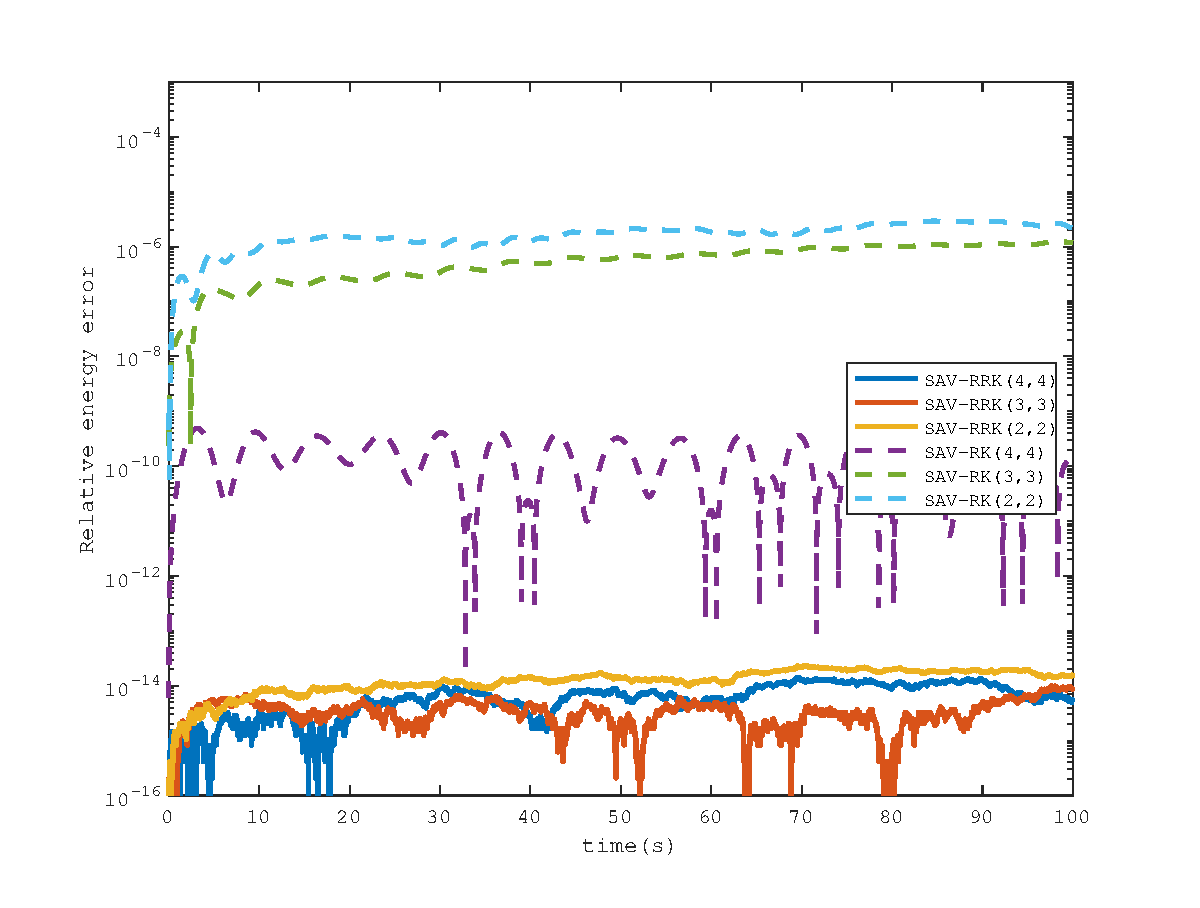
\includegraphics[width=0.5\textwidth]{./figures/exp4_energy2.eps}
	%\centerline{($a$) Temporal accuracy with $N=128.$}
	}\caption{ Relative errors of energy with $N=4, \tau=0.01$ for different $\alpha$ in Example \ref{exp_SAVRRK:4}.}
	\label{fig_SAVRRK:3-5}
	\end{center}
	\end{figure}
	\section{结论}\label{Section_SAVRRK: 7}
	在本文中,我们提出了一种开发二维分数非线性薛定谔波动方程高阶显式能量守恒数值方法的新途径。该方法基于最近引入的标量辅助变量方法和弛豫龙格-库塔方法。理论分析和数值结果支持了所提方案的守恒性质。
	更多的数值结果表明,所提方法对于其他类似的分数保守问题也是有效的,例如非线性分数波动方程和分数Klein-Gordon-Schr{\"o}dinger方程等。
	% {\color{purple}{值得注意的是,即使在其他相关文献中提到的偶数阶IDT方法可能表现出更高阶的现象在我们的二维计算示例中并没有观察到。这一发现是新颖的,但仍然是一个待解的问题。}}
	
	\section*{致谢}
	% 本工作得到四川省科技计划的支持(项目编号2020YJ0110、2022JDTD0019),中国国家自然科学基金(项目编号11801389)以及四川师范大学Laurent数学中心和国家-地方联合工程实验室系统可信性自动验证(项目编号ZD20220105)的支持。
	本工作得到四川省科技计划的支持(项目编号2022JDTD0019)以及四川师范大学Laurent数学中心和国家-地方联合工程实验室系统可信性自动验证(项目编号ZD20220105)的支持。	
	%% 附录部分是通过 \appendix 命令开始的;
	%% 然后附录部分就和普通章节一样处理
	% \appendix
	

% \section{NFSWE的SAV重构}\label{Section_SAVRRK: 2}
% 在本节中,我们回顾了开发高效节能方案来解决 NFSWE 的主要挑战在于非线性项的离散化.
% 正如我们所知,所有 RK 方法都保留任意线性不变量 \cite{griffithsNumericalMethodsOrdinary2010},辛 RK 方法保留任意二次不变量\cite{cooperStabilityRungeKuttaMethods1987}.
% 然而,没有 RK 方法可以保留任意多项式不变量的次数高于两个或非多项式非线性不变量 \cite{calvoNumericalSolutionIsospectral1997}.
% 在本节中,为了利用松弛 RK 方法的二次不变性保持特性,我们将采用新开发的标量辅助变量方法将高次能量重写为二次能量,
% 然后将 NFSWE 重新表述为允许二次能量函数的等效形式.

% 在介绍该方案之前,我们引入一个标量辅助变量 (SAV),即让
% \begin{equation}
% 	w(t)=\sqrt{H(t)+C_0} \text { with } H(t)=\frac{\beta}{2}\|u(\cdot, t)\|_{L^{4}}^{4} .
% \end{equation}
% 直接计算得出
% \begin{equation}
% 	   \begin{aligned}
% 		w_t & =\frac{1}{2 \sqrt{H(t)+C_0}} \frac{d H(t)}{d t} \\
% 		& =\frac{1}{2 \sqrt{H(t)+C_0}} \frac{d}{d t} \int_{\Omega} \frac{\beta}{2}|u|^{4}d \boldsymbol{x} \\
% 		& =\frac{\beta}{\sqrt{H(t)+C_0}} \int_{\Omega} |u|^2 \Re\left(u \bar{u}_t\right) d \boldsymbol{x} \quad\left(\frac{d|u|^2}{d t}=2 \Re\left(u \bar{u}_t\right)\right) \\
% 		& =\Re \int_{\Omega} \frac{\beta|u|^2 u \bar{u}_t}{\sqrt{H(t)+C_0}} d \boldsymbol{x} \\
% 		& =\Re\left(b(u), u_t\right) \quad\left(b(u)=\beta|u|^2 u / \sqrt{H(t)+C_0}\right)
% 		\end{aligned}\label{eq_SAVRRK:2-1}
% \end{equation}
% 其中 $\Re(\cdot)$ 表示取复数的实部,$(\cdot, \cdot)$ 表示对 $\Omega$ 的 $L^2$ 内积.因此,模型问题 \eqref{eq_SAVRRK:s1} 可以等价地改写为
% \begin{align}
% & u_t=v, \label{eq_SAVRRK:2-2}\\
% & v_t=-(-\Delta)^{\alpha / 2} u-\mathrm{i}\kappa v-b(u) w, \label{eq_SAVRRK:2-3}\\
% & w_t=\Re\left(b(u), u_t\right) .\label{eq_SAVRRK:2-4}
% \end{align}

% 与初始条件
% \begin{align}\label{eq_SAVRRK:31}
% u(\boldsymbol{x}, 0)=u_{0}(\boldsymbol{x}), \quad v(\boldsymbol{x}, 0)=u_{1}(\boldsymbol{x}), \quad w(0)=\sqrt{\frac{\beta}{2}\|u(\cdot, 0)\|_{L^{4}}^{4} +C_0}.
% \end{align}

% 对系统 \eqref{eq_SAVRRK:2-2}-\eqref{eq_SAVRRK:2-3} 分别取 $v_t$ 和 $u_t$ 的内积,将 \eqref{eq_SAVRRK:2-4} 乘以 $w(t )$,对得到的方程求和,最后在时间间隔 $[0, t]$ 上对实部进行积分,立即得到修改后的能量守恒定律
% \begin{equation}
% E(t)=\|v(\cdot, t)\|^2+\left\|(-\Delta)^{\frac{\alpha}{4}} u(\cdot, t)\right\|^{2}+w^2(t)=E(0)
% \end{equation}
% 这对应于具有周期边界的问题 \eqref{eq_SAVRRK:s1} 的原始能量守恒定律 \eqref{eq_SAVRRK:9}.
% \section{保结构空间离散化}\label{Section_SAVRRK: 3}

% % \subsection{Space Semi-discrete System}
% 注意到周期性边界条件,我们选择傅立叶拟谱方法对 NFSWEs \eqref{eq_SAVRRK:2-2}-\eqref{eq_SAVRRK:31} 进行空间离散化.%We develop a numerical method to solve the initial-periodic boundary value problem \eqref{eq_SAVRRK:s1} in a finite domain $\Omega \times(0, T)$.

% 不失一般性,我们设置$d=2$.
% %First, we introduce some notations.
% 对于正整数$M$甚至正整数$N_{x}$和$N_{y}$,表示$\tau={T}/{M},h_{x}={2 L}/{N_{ x}}, h_{y}={2 L}/{N_{y}}$.定义 $\Omega_{h}^{\tau}=\Omega_{h} \times \Omega_{\tau}$,其中 $\Omega_{h}=\left\{\left(x_{i}, y_{ j}\right) \mid i=0,1, \cdots, N_{x}\!-\!1;\right.\\ \left.j=0,1, \cdots, N_{y}\! -\!1\right\}$ 和 $\Omega_{\tau}=\left\{t_{m} \mid t_{m}=m \tau, 0 \leq m \leq M\right\}$,其中 $t_{m}=m \tau, x_{i}\!=\!-L i h_{x}$ 和 $y_{j}\!=\!-L j h_{y}$.
% 然后给出任何时间级别的相应向量形式
% \begin{align}\label{eq_SAVRRK:47}
% &U^m=\left(u_{0,0}^m, \cdots, u_{N_{x}-1,0}^m, u_{0,1}^m, \cdots, u_{N_{x}-1,1}^m, \cdots, u_{0, N_{y}-1}^m, \cdots, u_{N_{x}-1, N_{y}-1}^m\right)^{T}.\\
% &V^m=\left(v_{0,0}^m, \cdots, v_{N_{x}-1,0}^m, v_{0,1}^m, \cdots, v_{N_{x}-1,1}^m, \cdots, v_{0, N_{y}-1}^m, \cdots, v_{N_{x}-1, N_{y}-1}^m\right)^{T}.\\
% &W^m=w^m.
% \end{align}
% 对于任何网格函数 $u,v\in \Omega_{h}^{\tau}$,
% 将离散内积和相关的离散范数定义为
% \begin{align}\label{eq_SAVRRK:48}
% (u, v)=h_{x} h_{y} \sum_{i=0}^{N_{x}-1} \sum_{j=0}^{N_{y}-1} u_{i, j} \bar{v}_{i, j}, \quad\|u\|=(u, u)^{\frac{1}{2}}, \quad\|u\|_{\infty}=\sup _{\left(x_{i}, y_{j}\right) \in \Omega_{h}}\left|u_{i, j}\right|.
% \end{align}

% 令 $\left(x_{i}, y_{j}\right) \in \Omega_{h}$ 为傅里叶配置点.表示 $u_{N}(x, y)$ 是
% $u(x, y)$ 的插值多项​​式函数,那么我们有
% \begin{align}\label{eq_SAVRRK:50}
% u_{N}(x, y)=\sum_{k_{1}=-N_{x} / 2}^{N_{x} / 2} \sum_{k_{2}=-N_{y} / 2}^{N_{y} / 2} \tilde{u}_{k_{1}, k_{2}} e^{\mathrm{i}\mu\left( k_{1} (x+L)+k_{2}(y+L)\right)},
% \end{align}
% 其中$\mu={\pi}/{L}$,以及系数
% \begin{align}\label{eq_SAVRRK:51}
% \tilde{u}_{k_{1}, k_{2}}=\frac{1}{N_{x} c_{k_{1}}} \frac{1}{N_{y} c_{k_{2}}} \sum_{l_1=0}^{N_{x}-1} \sum_{l_2=0}^{N_{y}-1} u(x_{l_1}, y_{l_2}) e^{-\mathrm{i}\mu\left( k_{1}(x_{l_1}+L)+k_{2}(y_{l_2}+L)\right)},
% \end{align}
% 其中 $c_{k_{1}}=1$ 对于 $\left|k_{1}\right|<N_{x} / 2, c_{k_{2}}=1$ 对于 $\left|k_{2 }\right|<N_{y} / 2, c_{k_{1}}=2$ 对于 $k_{1}=\pm N_{x} / 2$, $c_{k_{2}}=2$对于$ k_{2}=\pm N_{y} / 2$.
% 因此,分数拉普拉斯算子 $-(-\Delta)^{\frac{\alpha}{2}} u(x, y)$ 可以近似为
% \begin{align}\label{eq_SAVRRK:52}
% -(-\Delta)^{\frac{\alpha}{2}} u_{N}\left(x, y\right)=-\sum\limits_{k_{1}=-N_{x} / 2}^{N_{x} / 2} \sum\limits_{k_{2}=-N_{y} / 2}^{N_{y} / 2}\left|\left(k_{1} \mu\right)^{2}+\left(k_{2} \mu\right)^{2}\right|^{\frac{\alpha}{2}} \tilde{u}_{k_{1}, k_{2}} e^{\mathrm{i}\mu\left( k_{1} (x+L)+k_{2}(y+L)\right)},
% \end{align}
% % where $\sum\limits_{\mathbf{k}=-\mathbf{N} / 2}^{\mathbf{N} / 2}=\sum\limits_{k_{1}=-N_{x} / 2}^{N_{x} / 2} \sum\limits_{k_{2}=-N_{y} / 2}^{N_{y} / 2}, \mathbf{k} \cdot(\boldsymbol{x}+\mathbf{L})=k_{1}(x+L)+k_{2}(y+L)$.
% %We denote $u_{i, j}=u\left(x_{i}, y_{j}\right), \mu^{2} \cdot \mathbf{k}^{2}=\mu^{2}\left(k_{1}^{2}+k_{2}^{2}\right)$ and
% 将 \eqref{eq_SAVRRK:51} 插入 \eqref{eq_SAVRRK:52},并考虑点 $(x_i,y_j)$ 处的结果方程给出
% \begin{align}
% &-(-\Delta)^{\frac{\alpha}{2}} u_{N}\left(x_{i}, y_{j}\right)\nonumber\\
% %=&-\sum\limits_{k_{1}=-N_{x} / 2}^{N_{x} / 2} \sum\limits_{k_{2}=-N_{y} / 2}^{N_{y} / 2}\left|\mu^{2} \cdot \mathbf{k}^{2}\right|^{\frac{\alpha}{2}}\left(\frac{1}{N_{x} %c_{k_{1}}} \frac{1}{N_{y} c_{k_{2}}} \sum\limits_{l_{1}=0}^{N_{x}-1} \sum\limits_{l_{2}=0}^{N_{y}-1}u_{l_{1}, l_{2}} e^{-\mathrm{i}\mu\left( %k_{1}(x_{l_1}+L)+k_{2}(y_{l_2}+L)\right)}\right) e^{\mathrm{i} \mu\left(k_{1}\left(x_{i}+L\right)+k_{2}\left(y_{j}+L\right)\right)}\nonumber\\
% =&\sum\limits_{l_{1}=0}^{N_{x}-1} \sum\limits_{l_{2}=0}^{N_{y}-1}u(x_{l_{1}}, y_{l_{2}})\left(-\sum\limits_{k_{1}=-N_{x} / 2}^{N_{x} / 2} \sum\limits_{k_{2}=-N_{y} / 2}^{N_{y} / 2} \frac{1}{N_{x} c_{k_{1}}} \frac{1}{N_{y} c_{k_{2}}}\left|\mu^{2} \cdot \mathbf{k}^{2}\right|^{\frac{\alpha}{2}} e^{\mathrm{i} \mu\left(k_{1}\left(x_{i}-x_{l_{1}}\right)+k_{2}\left(y_{j}-y_{l_{2}}\right)\right)}\right)\nonumber\\
% =&\left(D^{\alpha}U\right)_{i+j N_{x}},\label{eq_SAVRRK:53}
% \end{align}
% % where $\mu^{2} \cdot \mathbf{k}^{2}=\mu^{2}\left(k_{1}^{2}+k_{2}^{2}\right), \boldsymbol{x_l}+\mathbf{L}=\left(x_{l_{1}}+L\right)+\left(y_{l_{2}}+L\right)$,
% 其中 $\mu^{2} \cdot \mathbf{k}^{2}=\mu^{2}\left(k_{1}^{2} k_{2}^{2}\right)$, $D^{\alpha}$ 是具有元素的谱对称微分矩阵
% \begin{align}\label{eq_SAVRRK:54}
% \left(D^{\alpha}\right)_{i+j N_{x}, l_{1}+l_{2} N_{x}}=-\sum\limits_{l_{1}=0}^{N_{x}-1} \sum\limits_{l_{2}=0}^{N_{y}-1}\frac{1}{N_{x} c_{k_{1}}} \frac{1}{N_{y} c_{k_{2}}}\left|\mu^{2} \cdot \mathbf{k}^{2}\right|^{\frac{\alpha}{2}} e^{\mathrm{i}\mu\left(k_{1}\left(x_{i}-x_{l_{1}}\right)+k_{2}\left(y_{j}-y_{l_{2}}\right)\right)}.
% \end{align}


% %\begin{remark}
% %	\label{rmk1}
% %	The spectral differential matrix $D^{\alpha}$ is a symmetric matrix with the elements
% %\begin{align}\label{eq_SAVRRK:54}
% %\left(D^{\alpha}\right)_{i+j N_{x}, l_{1}+l_{2} N_{x}}=-\sum_{\mathbf{k}=-\mathbf{N} / 2}^{\mathbf{N} / 2} \frac{1}{N_{x} c_{k_{1}}} \frac{1}{N_{y} c_{k_{2}}}\left|\mu^{2} \cdot \mathbf{k}^{2}\right|^{\frac{\alpha}{2}} e^{-i \mu\left(k_{1}\left(x_{i}-x_{l_{1}}\right)+k_{2}\left(y_{j}-y_{l_{2}}\right)\right)}.
% %\end{align}
% %\end{remark}

% % \begin{pf}
	
% % \begin{equation}
% % 	\begin{aligned}
% % 	\left(D^{S}\right)_{i+j N_{x}, l_{1}+l_{2} N_{x}} &=-\sum_{\mathbf{k}=-\mathbf{N} / 2}^{\mathbf{N} / 2} \frac{1}{N_{x} c_{k_{1}}} \frac{1}{N_{y} c_{k_{2}}}\left|\mu^{2} \cdot \mathbf{k}^{2}\right|^{\frac{\alpha}{2}} e^{-\mathrm{i} \mu\left(k_{1}\left(x_{i}-x_{l_{1}}\right)+k_{2}\left(y_{j}-y_{l_{2}}\right)\right)} \\
% % 	&=-\sum_{\mathbf{k}=-\mathbf{N} / 2}^{\mathbf{N} / 2} \frac{1}{N_{x} c_{k_{1}}} \frac{1}{N_{y} c_{k_{2}}}\left|\mu^{2} \cdot(-\mathbf{k})^{2}\right|^{\frac{\alpha}{2}} e^{-\mathrm{i} \mu\left(\left(-k_{1}\right)\left(x_{l_{1}}-x_{i}\right)+\left(-k_{2}\right)\left(y_{l_{2}}-y_{j}\right)\right)} \\
% % 	&=-\sum_{\mathbf{k}=-\mathbf{N} / 2}^{\mathbf{N} / 2} \frac{1}{N_{x} c_{k_{1}}} \frac{1}{N_{y} c_{k_{2}}}\left|\mu^{2} \cdot \mathbf{k}^{2}\right|^{\frac{\alpha}{2}} e^{-\mathrm{i} \mu\left(k_{1}\left(x_{l_{1}}-x_{i}\right)+k_{2}\left(y_{l_{2}}-y_{j}\right)\right)} \\
% % 	&=\left(D^{S}\right)_{l_{1}+l_{2} N_{x}, i+j N_{x}}
% % 	\end{aligned}
% % 	\label{eq_SAVRRK:55}\end{equation}
% % 	where we have used the fact that $c_{k_{1}}=1$ for $\left|k_{1}\right|<N_{x} / 2, c_{k_{2}}=1$ for $\left|k_{2}\right|<N_{y} / 2, c_{k_{1}}=2$ for $k_{1}=\pm N_{x} / 2$, and $c_{k_{1}}=2$ for $k_{2}=\pm N_{y} / 2 .$ The proof is complete.
% % \end{pf}

% 应用傅里叶拟谱法逼近前面空间中的等效系统\eqref{eq_SAVRRK:2-2}-\eqref{eq_SAVRRK:2-4},得到空间半离散系统如下
% \begin{align}
% 	& U_t=V, \label{eq_SAVRRK:3-9}\\
% 	& V_t=D^{\alpha} U-\mathrm{i}\kappa V- b(U) \cdot W, \label{eq_SAVRRK:3-10}\\
% 	& W_t=\Re\left(b(U), U_t\right) .\label{eq_SAVRRK:3-11}
% 	\end{align}

% 	具有初始条件 $U^0, V^0, W^0$,其中 $\cdot$ 表示向量之间的点乘.那么我们有下面的定理.
%     \begin{thm}	\label{thm3}
%         半离散系统\eqref{eq_SAVRRK:3-9}–\eqref{eq_SAVRRK:3-11}承认半离散全局二次能量守恒定律
%         % 	\begin{equation}
% % 		E(U,V,W):=\|V\|^2 - \left(U, D^{\alpha} U\right)+\left(W\right)^2 \equiv \text { Const. }
% % 		\end{equation}
% \begin{equation}
% 	E(U,V,W):=\|V\|^2 + \|D^\frac{\alpha}{2} U\|^2+\left(W\right)^2 \equiv \text { Const. }\label{eq_SAVRRK:313}
% 	\end{equation}
% \end{thm}

% \begin{pf}
%     对系统 \eqref{eq_SAVRRK:3-9}-\eqref{eq_SAVRRK:3-10} 分别取 $V_t$ 和 $U_t$ 的内积,
%     将 \eqref{eq_SAVRRK:3-11} 乘以 $W$,
% \begin{align}
% 	  \left(V_t, U_t\right)&=\left(V_t, V\right), \\
% 	 \left(V_t, U_t\right)&=\left(D^{\alpha} U, U_t\right)-i \kappa\left(V, U_t\right)-W\left(b(U), U_t\right), \\
% 	 W W_t&=W\Re\left(b(U), U_t\right),
% 	\end{align}
%     对得到的方程求和
% \begin{equation}
% 	\left(V_t, V\right) + W W_t= \left(D^{\alpha} U, U_t\right)-i \kappa\left(V, U_t\right)-W\left(b(U), U_t\right) + W\Re\left(b(U), U_t\right),
% \end{equation}
% 并取实部得到
% \begin{align}
% 	\Re\left(V_t, V\right) + \Re\left(W W_t\right)&= \Re\left(D^{\alpha} U, U_t\right)-\Re\left(i \kappa\left(V, U_t\right)\right)-W\Re\left(b(U), U_t\right) + W\Re\left(b(U), U_t\right),\\
% 	\Re\left(V_t, V\right) + \Re\left(W W_t\right)&= \Re\left(D^{\alpha} U, U_t\right).\label{eq_SAVRRK:319}
% \end{align}
% 很容易验证
% \begin{equation}
% 	\Re\left(V_t, V\right) = \frac{1}{2}\frac{d }{d t}\|V\|^2, \quad \Re\left(W W_t\right) = \frac{1}{2}\frac{d }{d t}\left(W\right)^2,\quad \Re\left(D^{\alpha} U, U_t\right)=-\frac{1}{2}\frac{d }{d t}\|D^\frac{\alpha}{2}U\|^2\label{eq_SAVRRK:320}
% \end{equation}
% 将方程\eqref{eq_SAVRRK:320}代入方程\eqref{eq_SAVRRK:319},可以得到
% \begin{equation}
% 	\frac{d }{d t}\left(\|V\|^2+\left(W\right)^2+\|D^\frac{\alpha}{2}U\|^2\right)=0.
% \end{equation}
% 这意味着方程\eqref{eq_SAVRRK:313}
% \end{pf}
% \section{守恒SAV-RRK格式}\label{Section_SAVRRK: 4}
% 为了加速计算,因此,我们采用SAV方法为NFSWEs提出了不变量保持的显式Runge-Kutta方案.本节开始,我们回顾RRK方法并讨论它们的结构保持特性.
% \subsection{Explicit SAV-RRK schemes}
% 为简洁起见,我们引入以下符号:
% \begin{equation}
% 	\bm{y}=\left(U,V,W\right)^T,\bm{y}_0=\left(U^0,V^0,W^0\right)^T , \bm{f}=(f^1,f^2,f^3)^T=(V,D^{\alpha} U-\mathrm{i}\kappa V-b(U)\cdot W,\Re\left(b(U), U_t\right))^T.
% \end{equation}
% 然后,NFSWEs\eqref{eq_SAVRRK:3-9}-\eqref{eq_SAVRRK:3-11} 可以重写为:
% \begin{equation}
% 	\left\{\begin{array}{l}
% 	\bm{y}_t=\bm{f}(\bm{y}),\quad t \in(0, T]\\
% 	\bm{y}(0)=\bm{y}_0.
% \end{array}\right.\label{eq_SAVRRK:3-121}
% \end{equation}
% 设 $\bm{y}^m$ 和 $\bm{y}^{m+1}$ 分别为 $\bm{y}\left(t_m\right)$ 和 $\bm{y}\left(t_{m+1}\right)$ 的数值逼近;应用于式 \eqref{eq_SAVRRK:3-121} 的 $s$ 阶显式 SAV-RK 方法的形式如下:
% \begin{equation}
% 	\left\{\begin{array}{l}
% 		\bm{Y}_{m i}=\bm{y}^m+\tau \sum\limits_{j=1}^i a_{i j} \bm{f}_{m j}, \quad i=1, \ldots, s, \\
% 		\bm{y}^{m+1}=\bm{y}^m+\tau \sum\limits_{i=1}^s b_i \bm{f}_{m i}
% 	\end{array}\right.\label{eq_SAVRRK:4-31}
% 	\end{equation}
%     其中 $m=0, \ldots, M-1$,$\bm{f}{m j}=\bm{f}\left(\bm{Y}{m j}\right)$,$j=1, \ldots, s$.以下是相关符号的定义:
% \begin{equation}
% \begin{aligned}
% A & =\left(a_{i j}\right)_{s \times s}, \quad a_{i j}=0 \quad \text { for } \quad j \geq i, \\
% b & =\left(b_1, \cdots, b_s\right)^T,
% \end{aligned}
% \end{equation}
% $s$ 阶 SAV-RK 方法可以用Butcher阵列表示,如下所示:
% \begin{equation}
% 	\begin{array}{c|c}
% 	c & A \\
% 	\hline \\
% 	& b^T
% 	\end{array}
% 	\end{equation}
%     其中,横坐标向量 $c$ 满足 $c_i=\sum\limits_{j=1}^s a_{i j}, i=1, \ldots, s$.

%     然而,众所周知,某些隐式 RK 方法可能是辛型的或代数稳定的,但是没有一种显式 RK 方法是辛型的或代数稳定的.这导致 SAV-RK 方法无法保持守恒性质.
    
%     考虑在区间 $\left[\hat{t}m, \hat{t}{m+1}\right], m \geq 0$ 上进行一步计算,设 $\bm{y}\gamma^m$ 和 $\bm{y}\gamma^{m+1}$ 分别是 $\bm{y}\left(\hat{t}m\right)$ 和 $\bm{y}\left(\hat{t}{m+1}\right)$ 的数值逼近,则式 \eqref{eq_SAVRRK:3-121} 的 $s$ 阶显式 SAV-RRK 方法定义如下:
%     \begin{equation}
% 	\left\{\begin{array}{l}
% 		\bm{Y}_{m i}=\bm{y}_\gamma^m+\tau \sum\limits_{j=1}^i a_{i j} \bm{f}_{m j}, \quad i=1, \ldots, s, \\
% 		\bm{y}_\gamma^{m+1}=\bm{y}_\gamma^m+\gamma_m \tau \sum\limits_{i=1}^s b_i \bm{f}_{m i}
% 	\end{array}\right.\label{eq_SAVRRK:4-3}
% 	\end{equation}
% % for $m=0, \ldots, M-1$, where $\bm{f}_{m j}=\bm{f}\left(\bm{Y}_{m j}\right)$, $j=1, \ldots, s$. With the following notations
% % \begin{equation}
% % \begin{aligned}
% % A & =\left(a_{i j}\right)_{s \times s}, \quad a_{i j}=0 \quad \text { for } \quad j \geq i, \\
% % b & =\left(b_1, \cdots, b_s\right)^T,
% % \end{aligned}
% % \end{equation}
% $s$ 阶 SAV-RRK 方法可以用Butcher阵列表示,如下所示:
% \begin{equation}
% 	\begin{array}{c|c}
% 	c & A \\
% 	\hline \\
% 	& \tilde{b}^T
% 	\end{array}
% 	\end{equation}
%     其中,$\tilde{b}=\gamma_m b$,$\gamma_m\neq 0$ 满足以下条件:
% \begin{equation}
% 	\left\{\begin{array}{ll}
% 	% E_{\gamma}^{m+1}=E_{\gamma}^{m}+2 \gamma_m \tau \sum\limits_{i=1}^s \Re\left\langle -\mathrm{i}\kappa V_{\gamma}^{m}+(1-\beta) b(U_{\gamma}^{m})\cdot W_{\gamma}^{m}, b_i \bm{f}_{m i}\right\rangle, &\text { if } \sum\limits_{i=1}^s b_i \bm{f}_{m i} \neq 0,\\
% 	E_{\gamma}^{m+1}=E_{\gamma}^{m}, &\text { if } \sum\limits_{i=1}^s b_i \bm{f}_{m i} \neq 0,\\
% 	\gamma_m=1, &\text { if } \sum\limits_{i=1}^s b_i \bm{f}_{m i} =0.
% 	\end{array}\right.\label{eq_SAVRRK:4-6}
% 	\end{equation}
%     在 $\hat{t}{m+1}$ 处,对数值解 $\bm{y}\gamma^{m+1}$ 可以有两种解释方式.

% 	\textbf{Incremental direction technique (IDT):} $\bm{y}_\gamma^{m+1}$ is viewed as the approximation to $\bm{y}\left(\hat{t}_m+\tau\right)$, then $\hat{t}_m=t_m, m \geq 0$.

% 	\textbf{Relaxation technique (RT):} $ \bm{y}_\gamma^{m+1}$ is viewed as the approximation to $\bm{y}\left(\hat{t}_m+\right.\left.\gamma_m \tau\right)$, then $\hat{t}_m$ may not be equal to $t_m$ when $m>0$.

% 需要指出的是,对数值解 $\bm{y}_\gamma^{m+1}$ 的不同理解将导致不同的收敛结果.

% 当且仅当 $\sum\limits_{i=1}^s b_i \bm{f}_{m i}\neq 0$ 时,$\gamma_m$ 的值也可以被明确地表达.经过简单的计算,我们可以得到:

% % \begin{equation}
% % 	\begin{aligned}
% % 	 E_{\gamma}^{m+1}  =&\|V_{\gamma}^{m+1}\|^2- \left(U_{\gamma}^{m+1}, D^{\alpha} U_{\gamma}^{m+1}\right)+\left(W_{\gamma}^{m+1}\right)^2 \\
% % 	 =&\|V_{\gamma}^{m}+\gamma_m\tau\sum\limits_{i=1}^{s}b_if_{mi}^2\|^2- \left(U_{\gamma}^{m}+\gamma_m\tau\sum\limits_{i=1}^{s}b_if_{mi}^1, D^{\alpha} \left(U_{\gamma}^{m}+\gamma_m\tau\sum\limits_{i=1}^{s}b_if_{mi}^1\right)\right)+\left(W_{\gamma}^{m}+\gamma_m\tau\sum\limits_{i=1}^{s}b_if_{mi}^3\right)^2\\
% % 	 =&\|V_{\gamma}^{m}\|^2- \left(U_{\gamma}^{m}, D^{\alpha} U_{\gamma}^{m}\right)+\left(W_{\gamma}^{m}\right)^2\\
% % 	 &+\left(V_{\gamma}^{m},\gamma_m\tau\sum\limits_{i=1}^{s}b_if_{mi}^2\right)+\left(\gamma_m\tau\sum\limits_{i=1}^{s}b_if_{mi}^2,V_{\gamma}^{m}\right)+\left(\gamma_m\tau\sum\limits_{i=1}^{s}b_if_{mi}^2,\gamma_m\tau\sum\limits_{i=1}^{s}b_if_{mi}^2\right)\\
% % 	 &- \left(U_{\gamma}^{m}, D^{\alpha} \left(\gamma_m\tau\sum\limits_{i=1}^{s}b_if_{mi}^1\right)\right)- \left(\gamma_m\tau\sum\limits_{i=1}^{s}b_if_{mi}^1, D^{\alpha}U_{\gamma}^{m}\right)\\
% % 	 &- \left(\gamma_m\tau\sum\limits_{i=1}^{s}b_if_{mi}^1, D^{\alpha}\left(\gamma_m\tau\sum\limits_{i=1}^{s}b_if_{mi}^1\right)\right)+2W_{\gamma}^{m}\gamma_m\tau\sum\limits_{i=1}^{s}b_if_{mi}^3+\left(\gamma_m\tau\sum\limits_{i=1}^{s}b_if_{mi}^3\right)^2\\
% % 	=& E_{\gamma}^{m}+\gamma_m\tau\left[\left(V_{\gamma}^{m},\sum\limits_{i=1}^{s}b_if_{mi}^2\right)+\left(\sum\limits_{i=1}^{s}b_if_{mi}^2,V_{\gamma}^{m}\right)\right.\\
% % 	&\left.-\left(U_{\gamma}^{m},D^{\alpha} \left(\sum\limits_{i=1}^{s}b_if_{mi}^1\right)\right)-\left(\sum\limits_{i=1}^{s}b_if_{mi}^1, D^{\alpha} U_{\gamma}^{m}\right)+2W_{\gamma}^{m}\sum\limits_{i=1}^{s}b_if_{mi}^3\right]\\
% % 	 &+\gamma_m^2\tau^2\left[\left(\sum\limits_{i=1}^{s}b_if_{mi}^2,\sum\limits_{i=1}^{s}b_if_{mi}^2\right)- \left(\sum\limits_{i=1}^{s}b_if_{mi}^1,D^{\alpha}\left(\sum\limits_{i=1}^{s}b_if_{mi}^1\right)\right)+\left(\sum\limits_{i=1}^{s}b_if_{mi}^3\right)^2\right].
% % 	\end{aligned}
% % 	\end{equation}
% \begin{equation}
% 	\begin{aligned}
% 	 E_{\gamma}^{m+1}  =&\|V_{\gamma}^{m+1}\|^2+\|D^\frac{\alpha}{2} U_{\gamma}^{m+1}\|^2+\left(W_{\gamma}^{m+1}\right)^2 \\
% 	 =&\|V_{\gamma}^{m+1}\|^2- \left(U_{\gamma}^{m+1}, D^{\alpha} U_{\gamma}^{m+1}\right)+\left(W_{\gamma}^{m+1}\right)^2 \\
% 	 =&\|V_{\gamma}^{m}+\gamma_m\tau\sum\limits_{i=1}^{s}b_if_{mi}^2\|^2- \left(U_{\gamma}^{m}+\gamma_m\tau\sum\limits_{i=1}^{s}b_if_{mi}^1, D^{\alpha} \left(U_{\gamma}^{m}+\gamma_m\tau\sum\limits_{i=1}^{s}b_if_{mi}^1\right)\right)+\left(W_{\gamma}^{m}+\gamma_m\tau\sum\limits_{i=1}^{s}b_if_{mi}^3\right)^2\\
% 	 =&\|V_{\gamma}^{m}\|^2+\|D^\frac{\alpha}{2} U_{\gamma}^{m}\|^2+\left(W_{\gamma}^{m}\right)^2\\
% 	 &+\left(V_{\gamma}^{m},\gamma_m\tau\sum\limits_{i=1}^{s}b_if_{mi}^2\right)+\left(\gamma_m\tau\sum\limits_{i=1}^{s}b_if_{mi}^2,V_{\gamma}^{m}\right)+\left\|\gamma_m\tau\sum\limits_{i=1}^{s}b_if_{mi}^2\right\|^2\\
% 	 &- \left(U_{\gamma}^{m}, D^{\alpha} \left(\gamma_m\tau\sum\limits_{i=1}^{s}b_if_{mi}^1\right)\right)- \left(\gamma_m\tau\sum\limits_{i=1}^{s}b_if_{mi}^1, D^{\alpha}U_{\gamma}^{m}\right)\\
% 	 &+ \left\|D^\frac{\alpha}{2}\left(\gamma_m\tau\sum\limits_{i=1}^{s}b_if_{mi}^1\right)\right\|^2+2W_{\gamma}^{m}\gamma_m\tau\sum\limits_{i=1}^{s}b_if_{mi}^3+\left(\gamma_m\tau\sum\limits_{i=1}^{s}b_if_{mi}^3\right)^2\\
% 	=& E_{\gamma}^{m}+\gamma_m\tau\left[\left(V_{\gamma}^{m},\sum\limits_{i=1}^{s}b_if_{mi}^2\right)+\left(\sum\limits_{i=1}^{s}b_if_{mi}^2,V_{\gamma}^{m}\right)\right.\\
% 	&\left.-\left(U_{\gamma}^{m},D^{\alpha} \left(\sum\limits_{i=1}^{s}b_if_{mi}^1\right)\right)-\left(\sum\limits_{i=1}^{s}b_if_{mi}^1, D^{\alpha} U_{\gamma}^{m}\right)+2W_{\gamma}^{m}\sum\limits_{i=1}^{s}b_if_{mi}^3\right]\\
% 	 &+\gamma_m^2\tau^2\left[\left\|\sum\limits_{i=1}^{s}b_if_{mi}^2\right\|^2+ \left\|D^\frac{\alpha}{2}\left(\sum\limits_{i=1}^{s}b_if_{mi}^1\right)\right\|^2+\left(\sum\limits_{i=1}^{s}b_if_{mi}^3\right)^2\right].
% 	\end{aligned}\label{eq_SAVRRK:49}
% 	\end{equation}
%     这个式子和 \eqref{eq_SAVRRK:4-6} 结合起来,得到:
% \begin{equation}
% \begin{aligned}
% 	&\gamma_m\tau\left[\left(V_{\gamma}^{m},\sum\limits_{i=1}^{s}b_if_{mi}^2\right)+\left(\sum\limits_{i=1}^{s}b_if_{mi}^2,V_{\gamma}^{m}\right)-\left(U_{\gamma}^{m},D^{\alpha} \left(\sum\limits_{i=1}^{s}b_if_{mi}^1\right)\right)-\left(\sum\limits_{i=1}^{s}b_if_{mi}^1, D^{\alpha} U_{\gamma}^{m}\right)+2W_{\gamma}^{m}\sum\limits_{i=1}^{s}b_if_{mi}^3\right]\\
% 	 &+\gamma_m^2\tau^2\left[\left\|\sum\limits_{i=1}^{s}b_if_{mi}^2\right\|^2+ \left\|D^\frac{\alpha}{2}\left(\sum\limits_{i=1}^{s}b_if_{mi}^1\right)\right\|^2+\left(\sum\limits_{i=1}^{s}b_if_{mi}^3\right)^2\right]=0,
% 	\end{aligned}
% \end{equation}
% 注意到 $\gamma_m \neq 0$,所以可以得到:
% \begin{equation}
% 	\gamma_m=-\frac{\left(V_{\gamma}^{m},\sum\limits_{i=1}^{s}b_if_{mi}^2\right)+\left(\sum\limits_{i=1}^{s}b_if_{mi}^2,V_{\gamma}^{m}\right)-\left(U_{\gamma}^{m},D^{\alpha} \left(\sum\limits_{i=1}^{s}b_if_{mi}^1\right)\right)-\left(\sum\limits_{i=1}^{s}b_if_{mi}^1, D^{\alpha} U_{\gamma}^{m}\right)+2W_{\gamma}^{m}\sum\limits_{i=1}^{s}b_if_{mi}^3}{\tau\left[\left\|\sum\limits_{i=1}^{s}b_if_{mi}^2\right\|^2+ \left\|D^\frac{\alpha}{2}\left(\sum\limits_{i=1}^{s}b_if_{mi}^1\right)\right\|^2+\left(\sum\limits_{i=1}^{s}b_if_{mi}^3\right)^2\right]} .
% % \gamma_m=\frac{\left(V_{\gamma}^{m}\right)^T \left(\sum\limits_{i=1}^{s}b_if_{mi}^2\right)+\left(\sum\limits_{i=1}^{s}b_if_{mi}^2\right)^T \left(V_{\gamma}^{m}\right)-\left(U_{\gamma}^{m}\right)^T D^{\alpha} \left(\sum\limits_{i=1}^{s}b_if_{mi}^1\right)-\left(\sum\limits_{i=1}^{s}b_if_{mi}^1\right)^T D^{\alpha} \left(U_{\gamma}^{m}\right)+2W_{\gamma}^{m}\sum\limits_{i=1}^{s}b_if_{mi}^3}{\tau\left[\left(\sum\limits_{i=1}^{s}b_if_{mi}^2\right)^T \left(\sum\limits_{i=1}^{s}b_if_{mi}^2\right)- \left(\sum\limits_{i=1}^{s}b_if_{mi}^1\right)^T D^{\alpha}\left(\sum\limits_{i=1}^{s}b_if_{mi}^1\right)+\left(\sum\limits_{i=1}^{s}b_if_{mi}^3\right)^2\right]} .
% \end{equation}
% 由于$\bm{y}_\gamma^{m+1}$可以被视为对$\bm{y}\left(\hat{t}_m+\gamma_m \tau\right)$的逼近,因此在每一步中确保$\gamma_m>0$非常重要.事实上,\eqref{eq_SAVRRK:4-6}中定义的$\gamma_m$对于小的步长$\tau$接近于$1$,这将在第\ref{Section_SAVRRK: 5-1}节进一步讨论.因此,松弛方法是良好定义的.

% % \subsection{Structure-preserving properties of the RRK methods}
% 在公式 \eqref{eq_SAVRRK:4-3} 中引入松弛系数 $\gamma_m$ 的目的是为了保证数值解的能量守恒.实验证明,SAV-RRK 方法对于守恒问题 \eqref{eq_SAVRRK:2-2}-\eqref{eq_SAVRRK:2-4} 是守恒的.
% \begin{thm}
% 	假设 SAV-RK 方法 \eqref{eq_SAVRRK:4-31} 至少为二阶方法;则对于足够小的步长 $\tau$,SAV-RRK 方法具有守恒性质
%     \begin{equation}
% 	E_{\gamma}^{m+1}=E_{\gamma}^{m}\label{eq_SAVRRK:4-10}
% \end{equation}
% 这种守恒性质适用于守恒问题.
% \end{thm}

% \begin{pf}
%     当 $\sum_{i=1}^s b_i \bm{f}{m i}=0$ 时,根据 \eqref{eq_SAVRRK:4-3} 中的第二个关系式可得 $\bm{y}\gamma^{m+1}=\bm{y}_\gamma^m$,从而自动满足性质 \eqref{eq_SAVRRK:4-10}.

%     当 $\sum_{i=1}^s b_i \bm{f}_{m i}\neq 0$ 时,根据条件 \eqref{eq_SAVRRK:4-6},性质 \eqref{eq_SAVRRK:4-10} 仍然成立.

% 由于 SAV-RK 方法的阶数至少为二,我们可以得出结论,在足够小的步长 $\tau$ 下,$\gamma_m>0$,这将在第 \ref{Section_SAVRRK: 5-1} 节中得到证明.
% \end{pf}

% \section{SAV-RRK 方法的精度}\label{Section_SAVRRK: 5}
% 本节中,我们将讨论 SAV-RRK 方法的精度.首先,我们估计松弛系数 $\gamma_m$,该系数在后续的分析中起着关键作用.然后,我们推导 SAV-RRK 方法的精度.

% \subsection{松弛系数的估计}\label{Section_SAVRRK: 5-1}

% 虽然松弛系数 $\gamma_m$ 往往会随着步数而变化,但是它在不同步数间可以通过类似的方式进行估计.在这里,我们只考虑区间 $\left[\hat{t}m, \hat{t}{m+1}\right]$ 内的单个步长.在此期间,$\sum_{i=1}^s b_i \bm{f}{m i}=0$ 的情况较为简单,因此我们将重点放在 $\sum{i=1}^s b_i \bm{f}_{m i} \neq 0$ 的情况下.

% 设
% % \begin{equation}
% % 	S_m(\gamma)=\|V_\gamma^{m+1}\|^2 + \|D^\frac{\alpha}{2} U_\gamma^{m+1}\|^2+\left(W_\gamma^{m+1}\right)^2-\|V_\gamma^{m}\|^2 - \|D^\frac{\alpha}{2} U_\gamma^{m}\|^2-\left(W_\gamma^{m}\right)^2,
% % \end{equation}
% \begin{equation}
% 	\begin{aligned}
% 		S_m(\gamma)=&\left\|V_\gamma^m+\gamma \tau \sum\limits_{i=1}^s b_i \bm{f}_{m i}^2\right\|^2 + \left\|D^\frac{\alpha}{2} \left(U_\gamma^m+\gamma \tau \sum\limits_{i=1}^s b_i \bm{f}_{m i}^1\right)\right\|^2\\
% 	&+\left(W_\gamma^m+\gamma \tau \sum\limits_{i=1}^s b_i \bm{f}_{m i}^3\right)^2-\|V_\gamma^{m}\|^2 - \|D^\frac{\alpha}{2} U_\gamma^{m}\|^2-\left(W_\gamma^{m}\right)^2,
% 	\end{aligned}
% 	\end{equation}
%     则,由 \eqref{eq_SAVRRK:4-6} 定义的 $\gamma_m$ 的值恰为函数 $S_m(\gamma)$ 的非零根.对于 $S_m(\gamma)$,我们有引理 \ref{lem_SAVRRK:5_1} 和引理 \ref{lem_SAVRRK:5_2}.

% \begin{lem}\label{lem_SAVRRK:5_1}
% 	假设 SAV-RK 方法 \eqref{eq_SAVRRK:4-31} 的阶数为 $p$,则对于足够小的 $\tau$,有以下结果成立:
%     \begin{equation}
% S_m(1)=\mathcal{O}\left(\tau^{p+1}\right)
% \end{equation}
% \end{lem} 
% \begin{pf}
% 	考虑以下初值问题:
% \begin{equation}
% \left\{\begin{array}{l}
% \tilde{\bm{y}}^{\prime}=\bm{f}(\tilde{\bm{y}}), \quad t \geq \hat{t}_m, \\
% \tilde{\bm{y}}\left(\hat{t}_m\right)=\bm{y}_\gamma^m,
% \end{array}\right.
% \end{equation}
% 其中,$\bm{y}\gamma^m$与式\eqref{eq_SAVRRK:4-3}中的相同.通过使用式\eqref{eq_SAVRRK:4-31}中$p$阶的SAV-RK方法进行一步计算,我们可以得到内部阶段$\tilde{Y}{m i}, i=1, \ldots, s$以及数值解$\tilde{\bm{y}}^{m+1}$,其满足当$\tau$足够小时,$\tilde{\bm{y}}^{m+1}=\tilde{\bm{y}}\left(\hat{t}m+\tau\right)+\mathcal{O}\left(\tau^{p+1}\right)$.利用$\bm{y}\gamma^m$,带$\gamma_m=1$的SAV-RRK方法\eqref{eq_SAVRRK:4-3}生成内部阶段$Y_{m i}, i=1, \ldots, s$和数值解$\bm{y}\gamma^{m+1}$.显然,$Y{m i}=\tilde{Y}{m i}, i=1, \ldots, s$,$\bm{y}\gamma^{m+1}=\tilde{\bm{y}}^{m+1}$.因此,令$\tilde{\bm{f}}{m i}:=\bm{f}\left(\tilde{Y}{m i}\right)$,我们有:
% \begin{equation}
% \begin{aligned}
% S_n(1) = &\|V_\gamma^{m+1}\|^2 + \|D^\frac{\alpha}{2} U_\gamma^{m+1}\|^2+\left(W_\gamma^{m+1}\right)^2-\|V_\gamma^{m}\|^2 - \|D^\frac{\alpha}{2} U_\gamma^{m}\|^2-\left(W_\gamma^{m}\right)^2 \\
% = &\|\tilde{V}^{m+1}\|^2 + \|D^\frac{\alpha}{2} \tilde{U}^{m+1}\|^2+\left(\tilde{W}^{m+1}\right)^2-\|\tilde{V}(\hat{t}_{m})\|^2 - \|D^\frac{\alpha}{2} \tilde{U}(\hat{t}_{m})\|^2-\left(\tilde{W}(\hat{t}_{m})\right)^2 \\
% = &\|\tilde{V}^{m+1}\|^2 -\|\tilde{V}(\hat{t}_{m}+\tau)\|^2 +\|\tilde{V}(\hat{t}_{m}+\tau)\|^2-\|\tilde{V}(\hat{t}_{m})\|^2\\
% & + \|D^\frac{\alpha}{2} \tilde{U}^{m+1}\|^2 -\|D^\frac{\alpha}{2} \tilde{U}(\hat{t}_{m}+\tau)\|^2+\|D^\frac{\alpha}{2} \tilde{U}(\hat{t}_{m}+\tau)\|^2- \|D^\frac{\alpha}{2} \tilde{U}(\hat{t}_{m})\|^2\\
% & +\left(\tilde{W}^{m+1}\right)^2 -\left(\tilde{W}(\hat{t}_{m}+\tau)\right)^2+\left(\tilde{W}(\hat{t}_{m}+\tau)\right)^2-\left(\tilde{W}(\hat{t}_{m})\right)^2 \\
% = &\mathcal{O}\left(\tau^{p+1}\right) +2\int_{\hat{t}_m}^{\hat{t}_m+\tau}\left[\Re\left(V_t, V\right) + \Re\left(W W_t\right) - \Re\left(D^{\alpha} U, U_t\right)\right].
% \end{aligned}\label{eq_SAVRRK:54}
% \end{equation}
% 将式\eqref{eq_SAVRRK:54}和式\eqref{eq_SAVRRK:319}结合起来,即可完成证明.
% \end{pf} 
% \textcolor{red}{
% \begin{lem}\label{lem_SAVRRK:5_2}
% 	假设SAV-RK方法\eqref{eq_SAVRRK:4-31}的阶数至少为2,则对于足够小的$\tau$,有:
%     \begin{equation}
% S_m^{\prime}(0)=-c \tau^2+\mathcal{O}\left(\tau^3\right) \text { and } S_n^{\prime}(1)=c \tau^2+\mathcal{O}\left(\tau^3\right)
% \end{equation}
% 其中$c$是一个正常数.
% \end{lem} 
% \begin{pf}
% 	Similar to \eqref{eq_SAVRRK:49}
% 	\begin{equation}
% 		\begin{aligned}
% 			S_m(\gamma)=&\gamma\tau\left[\left(V_{\gamma}^{m},\sum\limits_{i=1}^{s}b_if_{mi}^2\right)+\left(\sum\limits_{i=1}^{s}b_if_{mi}^2,V_{\gamma}^{m}\right)-\left(U_{\gamma}^{m},D^{\alpha} \left(\sum\limits_{i=1}^{s}b_if_{mi}^1\right)\right)-\left(\sum\limits_{i=1}^{s}b_if_{mi}^1, D^{\alpha} U_{\gamma}^{m}\right)+2W_{\gamma}^{m}\sum\limits_{i=1}^{s}b_if_{mi}^3\right]\\
% 			 &+\gamma^2\tau^2\left[\left\|\sum\limits_{i=1}^{s}b_if_{mi}^2\right\|^2+ \left\|D^\frac{\alpha}{2}\left(\sum\limits_{i=1}^{s}b_if_{mi}^1\right)\right\|^2+\left(\sum\limits_{i=1}^{s}b_if_{mi}^3\right)^2\right].
% 			\end{aligned}
% 		\end{equation}	
%         一个直接的计算可以得到:
% \begin{equation}
% \begin{aligned}
% S_m^{\prime}(\gamma)=&\tau\left[\left(V_{\gamma}^{m},\sum\limits_{i=1}^{s}b_if_{mi}^2\right)+\left(\sum\limits_{i=1}^{s}b_if_{mi}^2,V_{\gamma}^{m}\right)-\left(U_{\gamma}^{m},D^{\alpha} \left(\sum\limits_{i=1}^{s}b_if_{mi}^1\right)\right)-\left(\sum\limits_{i=1}^{s}b_if_{mi}^1, D^{\alpha} U_{\gamma}^{m}\right)+2W_{\gamma}^{m}\sum\limits_{i=1}^{s}b_if_{mi}^3\right]\\
% &+2\gamma\tau^2\left[\left\|\sum\limits_{i=1}^{s}b_if_{mi}^2\right\|^2+ \left\|D^\frac{\alpha}{2}\left(\sum\limits_{i=1}^{s}b_if_{mi}^1\right)\right\|^2+\left(\sum\limits_{i=1}^{s}b_if_{mi}^3\right)^2\right].
% \end{aligned}
% \end{equation}
% 因此,我们有:
% \begin{equation}
% 	\begin{aligned}
% 	S_m^{\prime}(0)=&\tau\left[\left(V_{\gamma}^{m},\sum\limits_{i=1}^{s}b_if_{mi}^2\right)+\left(\sum\limits_{i=1}^{s}b_if_{mi}^2,V_{\gamma}^{m}\right)-\left(U_{\gamma}^{m},D^{\alpha} \left(\sum\limits_{i=1}^{s}b_if_{mi}^1\right)\right)-\left(\sum\limits_{i=1}^{s}b_if_{mi}^1, D^{\alpha} U_{\gamma}^{m}\right)+2W_{\gamma}^{m}\sum\limits_{i=1}^{s}b_if_{mi}^3\right]
% 	\end{aligned}
% 	\end{equation}
% 和
% \begin{equation}
% 	\begin{aligned}
% 	S_m^{\prime}(1)=&\tau\left[\left(V_{\gamma}^{m},\sum\limits_{i=1}^{s}b_if_{mi}^2\right)+\left(\sum\limits_{i=1}^{s}b_if_{mi}^2,V_{\gamma}^{m}\right)-\left(U_{\gamma}^{m},D^{\alpha} \left(\sum\limits_{i=1}^{s}b_if_{mi}^1\right)\right)-\left(\sum\limits_{i=1}^{s}b_if_{mi}^1, D^{\alpha} U_{\gamma}^{m}\right)+2W_{\gamma}^{m}\sum\limits_{i=1}^{s}b_if_{mi}^3\right]\\
% 	&+2\tau^2\left[\left\|\sum\limits_{i=1}^{s}b_if_{mi}^2\right\|^2+ \left\|D^\frac{\alpha}{2}\left(\sum\limits_{i=1}^{s}b_if_{mi}^1\right)\right\|^2+\left(\sum\limits_{i=1}^{s}b_if_{mi}^3\right)^2\right].
% 	\end{aligned}
% 	\end{equation}
% 	存在$\tilde{t}_m \in$ $\left[\hat{t}_m, \hat{t}_m+\tau\right]$,使得$\bm{f}\left(\bm{y}\left(\tilde{t}_m\right)\right) \neq 0$.使用简写符号$\tilde{\bm{f}}_m=\bm{f}\left(\bm{y}\left(\tilde{t}m\right)\right))$并进行Taylor展开,我们有$\bm{f}{m i}=\tilde{\bm{f}}_m+\mathcal{O}(\tau)$,当$\tau$足够小时成立.因此,有:
%     \begin{equation}
% 	\begin{aligned}
% 	S_m^{\prime}(0)=&\tau\left[\left(V_{\gamma}^{m},\sum\limits_{i=1}^{s}b_i\tilde{f}_m^2\right)+\left(\sum\limits_{i=1}^{s}b_i\tilde{f}_m^2,V_{\gamma}^{m}\right)-\left(U_{\gamma}^{m},D^{\alpha} \left(\sum\limits_{i=1}^{s}b_i\tilde{f}_m^1\right)\right)-\left(\sum\limits_{i=1}^{s}b_i\tilde{f}_m^1, D^{\alpha} U_{\gamma}^{m}\right)+2W_{\gamma}^{m}\sum\limits_{i=1}^{s}b_i\tilde{f}_m^3\right]\\
% 	&+\mathcal{O}(\tau^2)\\
% 	=&c\tau+\mathcal{O}(\tau^2)
% 	\end{aligned}
% 	\end{equation}
% 以及
% \begin{equation}
% 	\begin{aligned}
% 	S_m^{\prime}(1)=&\tau\left[\left(V_{\gamma}^{m},\sum\limits_{i=1}^{s}b_i\tilde{f}_m^2\right)+\left(\sum\limits_{i=1}^{s}b_i\tilde{f}_m^2,V_{\gamma}^{m}\right)-\left(U_{\gamma}^{m},D^{\alpha} \left(\sum\limits_{i=1}^{s}b_i\tilde{f}_m^1\right)\right)-\left(\sum\limits_{i=1}^{s}b_i\tilde{f}_m^1, D^{\alpha} U_{\gamma}^{m}\right)+2W_{\gamma}^{m}\sum\limits_{i=1}^{s}b_i\tilde{f}_m^3\right]\\
% 	&+2\tau^2\left[\left\|\sum\limits_{i=1}^{s}b_i\tilde{f}_m^2\right\|^2+ \left\|D^\frac{\alpha}{2}\left(\sum\limits_{i=1}^{s}b_i\tilde{f}_m^1\right)\right\|^2+\left(\sum\limits_{i=1}^{s}b_i\tilde{f}_m^3\right)^2\right]+\mathcal{O}(\tau^2)\\
% 	=&c\tau+\mathcal{O}(\tau^2).
% 	\end{aligned}
% 	\end{equation}
% \end{pf} }

% 结合引理\ref{lem_SAVRRK:5_1}和引理\ref{lem_SAVRRK:5_2},我们可以得到定义在\eqref{eq_SAVRRK:4-3}中的松弛系数$\gamma_m$的估计,详见定理\ref{thm_SAVRRK:5_1}.

% \begin{thm}\label{thm_SAVRRK:5_1}
% 	Suppose the order of SAV-RK method \eqref{eq_SAVRRK:4-31} is $p(p \geq 2)$; then, for sufficiently small $\tau$, the relaxation coefficient $\gamma_m$ defined in \eqref{eq_SAVRRK:4-6} satisfies
% \begin{equation}\label{eq_SAVRRK:5_3}
% \gamma_m=1+\mathcal{O}\left(\tau^{p-1}\right)
% \end{equation}
% \end{thm} 
% \begin{pf}
% 	在$\sum_{i=1}^s b_i \bm{f}{m i}=0$的情况下,我们有$\gamma_m=1$,它自动满足\eqref{eq_SAVRRK:5_3}.在$\sum{i=1}^s b_i \bm{f}_{m i}\neq 0$的情况下,注意到$S_m(\gamma)$是$\gamma$的二次函数,并利用以下事实:
%     \begin{equation}
% \begin{aligned}
% & S_m(0)=0, \quad S_m(1)=\mathcal{O}\left(\tau^{p+1}\right), \\
% & S_m^{\prime}(0)=-c \tau^2+\mathcal{O}\left(\tau^3\right), \quad S_m^{\prime}(1)=c \tau^2+\mathcal{O}\left(\tau^3\right) \quad \text { with } c>0, \\
% &
% \end{aligned}
% \end{equation}
% 我们可以推导出$S_m(\gamma)$的一个根$\gamma=1+\mathcal{O}\left(\tau^{p-1}\right)$.因此,定义在\eqref{eq_SAVRRK:4-6}中的松弛系数$\gamma_m$满足\eqref{eq_SAVRRK:5_3},从而完成了证明.
% \end{pf}
% \begin{remark}\label{rk_SAVRRK:5_1}
% 	定理\ref{thm_SAVRRK:5_1}中的结果表明,对于足够小的$\tau$,松弛系数$\gamma_m$接近于$1$,这意味着松弛方法可以被视为标准方法的小扰动.
% \end{remark}
% \subsection{SAV-RRK方法的截断误差}
% 现在我们进一步研究使用松弛系数$\gamma_m$的估计来研究SAV-RRK方法的精度.在证明方法的精度之前,我们将方案\eqref{eq_SAVRRK:4-3}重写为
% \begin{equation}
% 	\left\{\begin{array}{l}
% 		\bm{Y}_{m i}=\bm{y}_\gamma^m+\tau \sum\limits_{j=1}^i a_{i j} \bm{f}_{m j}, \quad i=1, \ldots, s, \\
% 		\bm{y}_\gamma^{m+1}=\bm{y}_\gamma^m+\gamma_m \tau \sum\limits_{i=1}^s b_i \bm{f}_{m i}\\
% 		\bm{y}_\gamma^{m+1}=\bm{y}^{m+1}+\left(\gamma_m-1\right)\left(\bm{y}^{m+1}-\bm{y}_\gamma^m\right) .
% 	\end{array}\right.\label{eq_SAVRRK:4-321}
% 	\end{equation}
%     我们遵循 \cite{ranochaGeneralRelaxationMethods2020} 中引理 $2.7$ 证明的思路,得到以下结果.

% \begin{thm}\label{thm_SAVRRK:5_4}
% 假设 SAV-RK 方法 \eqref{eq_SAVRRK:4-31} 的阶数为 $p (p \geq 2)$,则以下陈述成立:
% 对于 IDT,即将 $\bm{y}_\gamma^{m+1}$ 视为在 $\hat{t}_m+\tau$ 处的近似值,SAV-RRK 方法 \eqref{eq_SAVRRK:4-3} 的阶数为 $p-1$.

% 对于 RT,即将 $\bm{y}_\gamma^{m+1}$ 视为在 $\hat{t}_m+\gamma_m \tau$ 处的近似值,SAV-RRK 方法 \eqref{eq_SAVRRK:4-3} 的阶数为 $p$.
% \end{thm} 
% \begin{pf}
% 	设 $\hat{t}_{m i}=\hat{t}_m+c_i \tau, i=1, \ldots, s$,并将精确解代入 \eqref{eq_SAVRRK:4-321} 中的第二个式子,可以得到:
%     \begin{equation}
% \bm{y}\left(\hat{t}_m+\tau\right)\bm{y}\left(\hat{t}_m\right)+\tau \sum_{i=1}^s b_i \bm{f}\left(\bm{y}\left(\hat{t}_{m i}\right)\right)+\mathcal{O}\left(\tau^{p+1}\right),
% \end{equation}
% 这些公式是从 SAV-RK 方法 \eqref{eq_SAVRRK:4-31} 的精度导出的.然后,我们估计 \eqref{eq_SAVRRK:4-321} 中第三个式子的截断误差.将精确解代入该式子,并记 $\phi_m(\bm{y}(t)):=\bm{y}\left(\hat{t}m\right)+\tau \sum{i=1}^s b_i \bm{f}\left(\bm{y}\left(\hat{t}_{m i}\right)\right)$,得到:
% \begin{equation}
% 	\bm{y}\left(\hat{t}_{m+1}\right)=\phi_m(\bm{y}(t))+\left(\gamma_m-1\right)\left(\phi_m(\bm{y}(t))-\bm{y}\left(\hat{t}_m\right)\right)+d_{m+1} .
% \end{equation}
% 显然,利用 $\gamma_m=1+\mathcal{O}\left(\tau^{p-1}\right)$ 这个事实,可以得到:
% \begin{equation}
% 	\begin{aligned}
% 		d_{m+1}= & \bm{y}\left(\hat{t}_{m+1}\right)-\phi_m(\bm{y}(t))-\left(\gamma_m-1\right)\left(\phi_m(\bm{y}(t))-\bm{y}\left(\hat{t}_m\right)\right) \\
% 		= & \bm{y}\left(\hat{t}_{m+1}\right)-\left(\bm{y}\left(\hat{t}_m+\tau\right)+\mathcal{O}\left(\tau^{p+1}\right)\right)-\left(\gamma_m-1\right)\left(\bm{y}\left(\hat{t}_m+\tau\right)+\mathcal{O}\left(\tau^{p+1}\right)-\bm{y}\left(\hat{t}_m\right)\right) \\
% 		= & \bm{y}\left(\hat{t}_{m+1}\right)-\bm{y}\left(\hat{t}_m+\tau\right)-\left(\gamma_m-1\right)\left(\bm{y}\left(\hat{t}_m+\tau\right)-\bm{y}\left(\hat{t}_m\right)\right) \\
% 		& +\mathcal{O}\left(\tau^{p+1}\right)+\mathcal{O}\left(\left(\gamma_m-1\right) \tau^{p+1}\right) \\
% 		= & \bm{y}\left(\hat{t}_{m+1}\right)-\bm{y}\left(\hat{t}_m+\tau\right)-\left(\gamma_m-1\right) \bm{y}^{\prime}\left(\hat{t}_m+\tau\right) \tau+\mathcal{O}\left(\left(\gamma_m-1\right) \tau^2\right)+\mathcal{O}\left(\tau^{p+1}\right) \\
% 		= & \bm{y}\left(\hat{t}_{m+1}\right)-\bm{y}\left(\hat{t}_m+\tau\right)-\left(\gamma_m-1\right) \bm{y}^{\prime}\left(\hat{t}_m+\tau\right) \tau+\mathcal{O}\left(\tau^{p+1}\right) .
% 		\end{aligned}
% 		\end{equation}
% 		对于 IDT,$\bm{y}_\gamma^{m+1}$ 被视为在 $\hat{t}m+\tau$ 处的近似值,因此 $\hat{t}{m+1}=\hat{t}m+\tau$,这意味着,利用 $\gamma_m$ 的估计,有 $d{n+1}=-\left(\gamma_m-1\right) \bm{y}^{\prime}\left(\hat{t}_m+\tau\right) \tau+\mathcal{O}\left(\tau^{p+1}\right)=$ $\mathcal{O}\left(\tau^p\right)$,因此该方法的阶数为 $p-1$.

% 对于 RT,由于 $\bm{y}_\gamma^{m+1}$ 被视为在 $\hat{t}m+\gamma_m \tau$ 处的近似值,$\hat{t}{m+1}=\hat{t}_m+\gamma_m \tau$.使用泰勒展开得到以下估计:
% \begin{equation}
% 		\begin{aligned}
% 		d_{m+1}= & \bm{y}\left(\hat{t}_m+\tau+\left(\gamma_m-1\right) \tau\right)-\bm{y}\left(\hat{t}_m+\tau\right)-\left(\gamma_m-1\right) y^{\prime}\left(\hat{t}_m+\tau\right) \tau+\mathcal{O}\left(\tau^{p+1}\right) \\
% 		= & \bm{y}\left(\hat{t}_m+\tau\right)+\left(\gamma_m-1\right) \bm{y}^{\prime}\left(\hat{t}_m+\tau\right) \tau+\mathcal{O}\left(\left(\gamma_m-1\right)^2 \tau^2\right) \\
% 		& -\bm{y}\left(\hat{t}_m+\tau\right)-\left(\gamma_m-1\right) \bm{y}^{\prime}\left(\hat{t}_m+\tau\right) \tau+\mathcal{O}\left(\tau^{p+1}\right) \\
% 		= & \mathcal{O}\left(\tau^{p+1}\right),
% 		\end{aligned}
% \end{equation}
% 由此可以得知该方法的阶数为 $p$.
% \end{pf}
% \begin{remark}\label{rk_SAVRRK:5_5}
% 	在实际计算中,IDT 方法的阶数可能会比我们预期的更高,甚至可以达到 RT 方法的阶数,这可以在例子 \ref{exp_SAVRRK:1} 中观察到.
% \end{remark}

% \section{数值算例}\label{Section_SAVRRK: 6}
% 为了支持和验证之前的理论结果,本节提供了一些数值例子. 在我们的计算中,采用了基于快速傅里叶变换(FFT)方法的快速求解器方法,可以减少内存需求和计算复杂度. 我们进行了几个实验来说明所提出的方法的有效性,并将它们与其他经典的SAV-RK方法进行比较. 首先,我们展示了SAV重构的RRKs和IDTs的数值收敛阶. 然后我们展示了所提出的方案的精度和守恒性质.

% 在数值测试中,将使用以下RK方法:
% \begin{enumerate}
% 	\item $\operatorname{RK}(2,2)$ : 二级、二阶 Heun 方法 %of \cite{shuEfficientImplementationEssentially1988}.
% \begin{equation}
% 	\begin{array}{c|cc}
% 	0 & 0 & 0 \\
% 	\frac{2}{3} & \frac{2}{3} & 0 \\
% 	\hline & \frac{1}{4} & \frac{3}{4}
% 	\end{array}
% 	\end{equation}

% 	\item $\mathrm{RK}(3,3)$ : 三级、三阶 Heun 方法 %of \cite{shuEfficientImplementationEssentially1988}.

% 	\begin{equation}
% 		\begin{array}{c|ccc}
% 		0 & 0 & 0 & 0 \\
% 		\frac{1}{3} & \frac{1}{3} & 0 & 0 \\
% 		\frac{2}{3} & 0 & \frac{2}{3} & 0 \\
% 		\hline & \frac{1}{4} & 0 & \frac{3}{4}
% 		\end{array}
% 		\end{equation}
	
%     \item $\operatorname{RK}(4,4)$ : 四级、四阶 Gill 方法 %of \cite{shuEfficientImplementationEssentially1988}.
	
% 	\begin{equation}
% 		\begin{array}{c|cccc}
% 		0 & 0 & 0 & 0 & 0 \\
% 		\frac{1}{2} & \frac{1}{2} & 0 & 0 & 0 \\
% 		\frac{1}{2} & \frac{\sqrt{2}-1}{2} & 1-\frac{\sqrt{2}}{2} & 0 & 0 \\
% 		1 & 0 & -\frac{\sqrt{2}}{2} & 1+\frac{\sqrt{2}}{2} & 0 \\
% 		\hline & \frac{1}{6} & \frac{2-\sqrt{2}}{6} & \frac{2+\sqrt{2}}{6} & \frac{1}{6}
% 		\end{array}
% 		\end{equation}
	
% \end{enumerate}

% 此外,还将使用SAV方法\cite{chengConvergenceEnergyconservingScheme2022}和三层线性隐式差分格式\cite{wangConservativeLinearizedDifference2015}进行比较. 为了得到数值误差,我们使用以下误差函数
% \begin{align}\label{eq_SAVRRK:103}
% Error(\tau)=\left\|U_{N}^{M}-U_{N}^{2 M}\right\|_{\infty},~Error(N)=\left\|U_{N}^{M}-U_{2 N}^{M}\right\|_{\infty},
% \end{align}
% 其中
% $$\left\|U_{N}^{M}-U_{N}^{2 M}\right\|_{\infty}=\left\|U\left(\frac{T}{M}, \frac{L}{N}\right)-U\left(\frac{T}{2 M}, \frac{L}{N}\right)\right\|_{\infty},\left\|U_{N}^{M}-U_{2 N}^{M}\right\|_{\infty}=\left\|U\left(\frac{T}{M}, \frac{L}{N}\right)-U\left(\frac{T}{M}, \frac{L}{2 N}\right)\right\|_{\infty},$$
% 并且在两个连续的时间步长$\tau$和$\tau / 2$和两个连续的多项式次数$N$和$2 N$上,通过以下公式计算时间和空间的收敛阶
% \begin{equation}
% \text { order }= \left\{
% \begin{aligned}
% \log _{2}[Error(\tau) / Error(\tau / 2)], & \text { in time } \\
% \log _{2}[Error(N) / Error(2 N)], & \text { in space. }
% \end{aligned}\right.\label{eq_SAVRRK:104}
% \end{equation}

% 为了描述守恒性能,能量的相对误差由以下公式计算
% \begin{equation}\label{eq_SAVRRK:105}
% R E^{m}=\left|\left(E^{m}-E^{0}\right) / E^{0}\right|,
% \end{equation}
% 其中$E^{m}$表示$t_m$时的离散能量.


% \begin{example}\label{exp_SAVRRK:1}
%     首先,我们将一维NFSWEs \eqref{eq_SAVRRK:s1}表示为
% \begin{equation}\label{eq_SAVRRK:108}
% u_{t t}+(-\Delta)^{\alpha / 2} u+\mathrm{i}u_t+|u|^2 u=0, \quad (x,t)\in  \Omega\times[0, T],
% \end{equation}
% 当 $u(x, 0)=(1+\mathrm{i}) x e^{-10(1-x)^2}$ 和 $u_t(x, 0)=0$.
% \end{example}

% 不难验证,初始值函数$u(x, 0)$沿着$x$从$x=1$处指数衰减为零.这意味着初始值函数在有界区间$\Omega$之外可以忽略不计.考虑到机器精度的限制, 这里,我们取$\Omega=(-25,25)$.

% 不失一般性,这里我们取$\alpha=1.5$和$T=100$来验证我们的理论分析结果. 
% 选择时间步长$\Delta t=0.1,0.05,0.025,0.0125,0.00625$,标准SAV-RK、SAV-RRK和SAV-IDT格式的相应误差和时间收敛率如表\ref{tab_SAVRRK:6-1}所示. 
% 我们可以看到,所有的SAV-RRK格式保持了与标准SAV-RK格式相同的收敛阶数,而SAV-IDT格式则表现出不同的行为. 
% SAV-IDT $(2,2)$和SAV-IDT $(4,4)$给出了比定理\ref{thm_SAVRRK:5_4}中指示的期望速率更高的收敛阶数,而SAV-IDT $(3,3)$则给出了降低了一个阶数的收敛速率. 
% 这种不同的行为可以归因于$\left|1-\gamma_n\right|$的收敛速率对于SAV-RRK(2, 2)和SAV-RRK(4, 4)提高了一个阶数,如图\ref{fig_SAVRRK:1}所示. 
% 同时,在步长重新缩放后,在大多数情况下,标准的SAV-RKs和SAV-RRKs给出了非常接近的数值误差.
% \begin{table}[H]\footnotesize
% 	\centering
% 	\caption{在$N=32, T = 100$时,SAV-RK、SAV-RRK和SAV-IDT的数值误差和收敛阶数(例 \ref{exp_SAVRRK:1}).}
% 	\begin{tabular}{lllllrlrlrlrlrl}
% 	\toprule
% 	\multicolumn{2}{l}{\multirow{2}[3]{*}{\textbf{RK(Stage,Order)}}} & \multicolumn{2}{l}{\multirow{2}[3]{*}{$\bm{\Delta t}$}} & \multicolumn{3}{c}{\textbf{SAV-RK}} &       & \multicolumn{3}{c}{\textbf{SAV-RRK}} &       & \multicolumn{3}{c}{\textbf{SAV-IDT}} \\
% 	\cmidrule{5-7}\cmidrule{9-11}\cmidrule{13-15}    \multicolumn{2}{l}{} & \multicolumn{2}{l}{} & \textbf{Error} &       & \textbf{order} &       & \textbf{Error} &       & \textbf{order} &       & \textbf{Error} &       & \textbf{order} \\
% 	\multicolumn{2}{l}{\multirow{5}[0]{*}{\textbf{RK(2,2)}}} & \multicolumn{2}{l}{0.1} & 1.8552E-04 &       & -     &       & 1.9063E-04 &       & -     &       & 2.0325E-04 &       & - \\
% 	\multicolumn{2}{l}{} & \multicolumn{2}{l}{0.05} & 4.6601E-05 &       & 1.9931  &       & 4.7240E-05 &       & 2.0126  &       & 5.0585E-05 &       & 2.0065  \\
% 	\multicolumn{2}{l}{} & \multicolumn{2}{l}{0.025} & 1.1671E-05 &       & 1.9974  &       & 1.1750E-05 &       & 2.0074  &       & 1.2387E-05 &       & 2.0298  \\
% 	\multicolumn{2}{l}{} & \multicolumn{2}{l}{0.0125} & 2.9200E-06 &       & 1.9990  &       & 2.9294E-06 &       & 2.0040  &       & 2.9549E-06 &       & 2.0677  \\
% 	\multicolumn{2}{l}{} & \multicolumn{2}{l}{0.00625} & 7.3022E-07 &       & 1.9996  &       & 7.3130E-07 &       & 2.0021  &       & 6.6665E-07 &       & 2.1481  \\
% 	\multicolumn{2}{l}{\multirow{5}[0]{*}{\textbf{RK(3,3)}}} & \multicolumn{2}{l}{0.1} & 7.6862E-06 &       & -     &       & 2.9857E-06 &       & -     &       & 1.7245E-04 &       & - \\
% 	\multicolumn{2}{l}{} & \multicolumn{2}{l}{0.05} & 9.5269E-07 &       & 3.0122  &       & 3.9037E-07 &       & 2.9352  &       & 4.3389E-05 &       & 1.9907  \\
% 	\multicolumn{2}{l}{} & \multicolumn{2}{l}{0.025} & 1.1866E-07 &       & 3.0052  &       & 5.0077E-08 &       & 2.9626  &       & 1.0873E-05 &       & 1.9966  \\
% 	\multicolumn{2}{l}{} & \multicolumn{2}{l}{0.0125} & 1.4809E-08 &       & 3.0023  &       & 6.3449E-09 &       & 2.9805  &       & 2.7208E-06 &       & 1.9986  \\
% 	\multicolumn{2}{l}{} & \multicolumn{2}{l}{0.00625} & 1.8497E-09 &       & 3.0011  &       & 7.9858E-10 &       & 2.9901  &       & 6.8049E-07 &       & 1.9994  \\
% 	\multicolumn{2}{l}{\multirow{5}[1]{*}{\textbf{RK(4,4)}}} & \multicolumn{2}{l}{0.1} & 3.7701E-07 &       & -     &       & 3.8894E-07 &       & -     &       & 7.0733E-07 &       & - \\
% 	\multicolumn{2}{l}{} & \multicolumn{2}{l}{0.05} & 2.3572E-08 &       & 3.9994  &       & 2.3939E-08 &       & 4.0221  &       & 4.4585E-08 &       & 3.9878  \\
% 	\multicolumn{2}{l}{} & \multicolumn{2}{l}{0.025} & 1.4730E-09 &       & 4.0003  &       & 1.4843E-09 &       & 4.0115  &       & 2.8080E-09 &       & 3.9889  \\
% 	\multicolumn{2}{l}{} & \multicolumn{2}{l}{0.0125} & 9.2041E-11 &       & 4.0003  &       & 9.2397E-11 &       & 4.0058  &       & 1.7743E-10 &       & 3.9842  \\
% 	\multicolumn{2}{l}{} & \multicolumn{2}{l}{0.00625} & 5.7518E-12 &       & 4.0002  &       & 5.7630E-12 &       & 4.0029  &       & 1.1309E-11 &       & 3.9718  \\
% 	\bottomrule
% 	  \end{tabular}%
% 	\label{tab_SAVRRK:6-1}%
%   \end{table}%
  
%   接下来,我们对每一步中的松弛系数 $\gamma_n$ 进行了充分的研究.我们计算了在不同时间步长 $\tau$ 的模拟过程中 $\gamma_m$ 和 1 之间的最大距离,即 $\max _m\left|\gamma_m-1\right|$,并且也计算了 $\left|S_m(1)\right|$ 的最大值,即 $\max _m\left|S_m(1)\right|$.一些松弛(RT)方法的数值结果如图 \ref{fig_SAVRRK:1} 所示.从图中可以看出,上述两个量的阶数与理论结果一致.这证实了引理 \ref{lem_SAVRRK:5_1} 和定理 \ref{thm_SAVRRK:5_1} 中的理论结果\begin{figure}[H]
% 	\begin{center}
% 	\subfigure[$\max _m\left|\gamma_m-1\right|$]{ \centering
% 	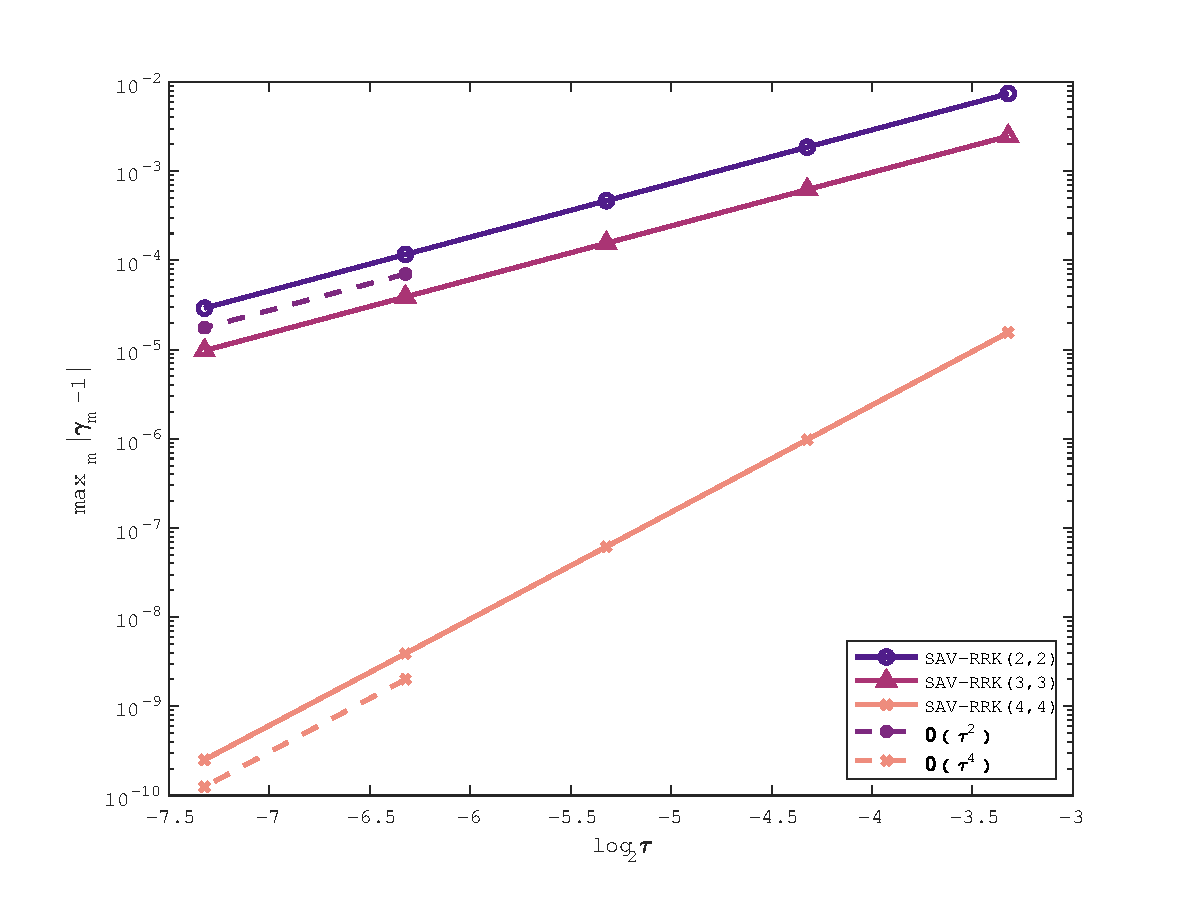
\includegraphics[width=0.5\textwidth]{./figures/exp1_r.eps}
% 	%\centerline{($b$) Spatial accuracy with $\tau = 10^{-3}.$}
% 	}\subfigure[$\max_m\left|S_m(1)\right|$]{ \centering
% 	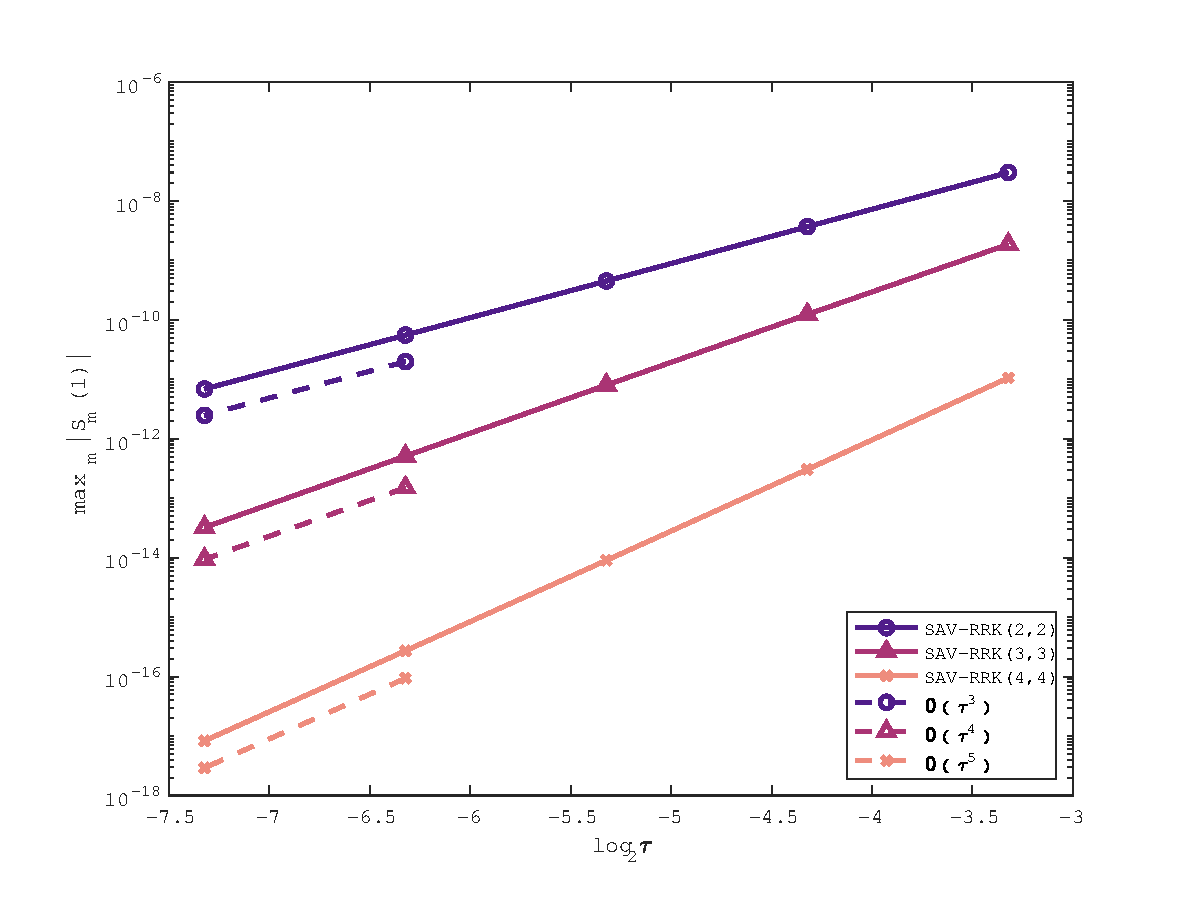
\includegraphics[width=0.5\textwidth]{./figures/exp1_s.eps}
% 	%\centerline{($a$) Temporal accuracy with $N=128.$}
% 	}\caption{松弛(RT)方法的 $\max _m\left|\gamma_m-1\right|$ 和 $\max_m\left|S_m(1)\right|$ (例 \ref{exp_SAVRRK:1})} 
% 	\label{fig_SAVRRK:1}
% 	\end{center}
% 	\end{figure}
  
%     此外,我们采用 $RK(4,4)$ 方法,计算不同 $\alpha$ 下的 $L^{\infty}$-范数误差.图 \ref{fig_SAVRRK:2} 显示了解的误差及其在 $L^{\infty}$-范数下的收敛阶数,结果证实了 SAV-IDT 方案和 SAV-RRK 方案在时间方向上都具有四阶收敛性.我们在图 \ref{fig_SAVRRK:3} 中描绘了不同 $N$ 和 $\tau=0.01$ 的方案的空间误差,结果显示出所提出的方案的空间误差非常小,几乎可以忽略不计,而误差主要由时间离散化误差所主导.这证实了对于充分光滑的问题,傅里叶拟谱方法在空间上是任意阶的.
%     \begin{figure}[H]
% 		\begin{center}
% 		\subfigure[$N=32 $(IDT)]{ \centering
% 		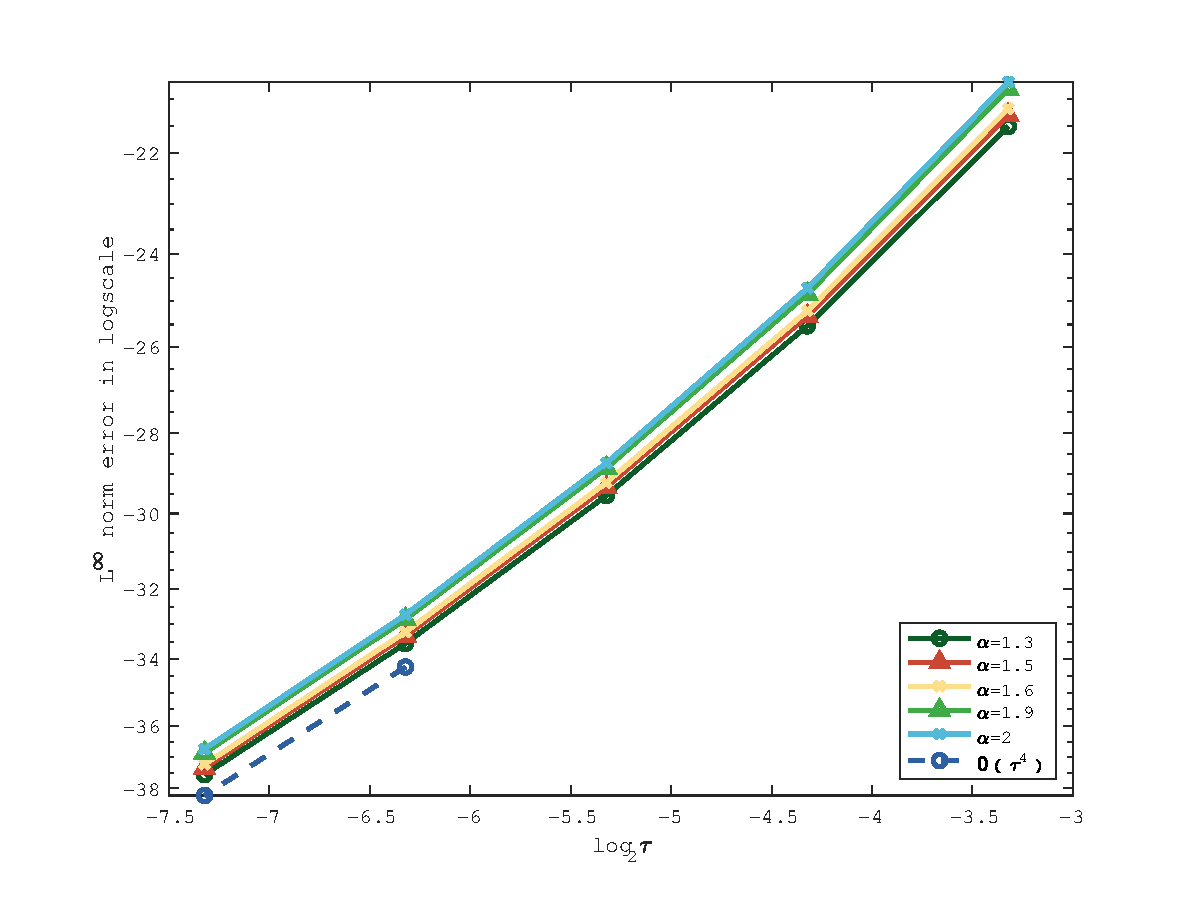
\includegraphics[width=0.5\textwidth]{./figures/exp1_RT_order_t.eps}
% 		%\centerline{($b$) Spatial accuracy with $\tau = 10^{-3}.$}
% 		}\subfigure[$N=32 $(RT)]{ \centering
% 		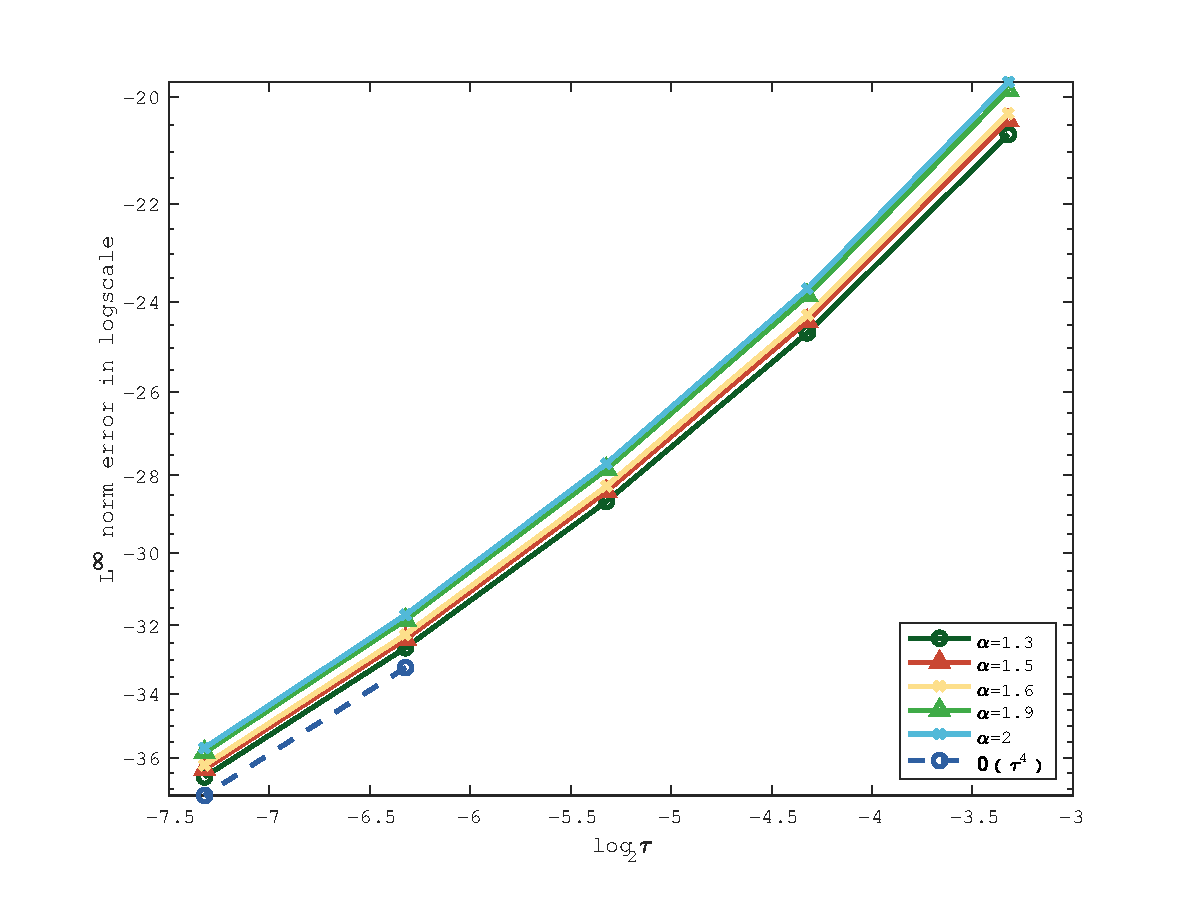
\includegraphics[width=0.5\textwidth]{./figures/exp1_IDT_order_t.eps}
% 		%\centerline{($a$) Temporal accuracy with $N=128.$}
% 		}\caption{不同 $\alpha$ 下 IDT 和 RT 的收敛阶数. (例 \ref{exp_SAVRRK:1})} 
% 		\label{fig_SAVRRK:2}
% 		\end{center}
% 		\end{figure}
% 	\begin{figure}[H]
% 		\begin{center}
% 		\subfigure[$\tau=0.01 $(IDT)]{ \centering
% 		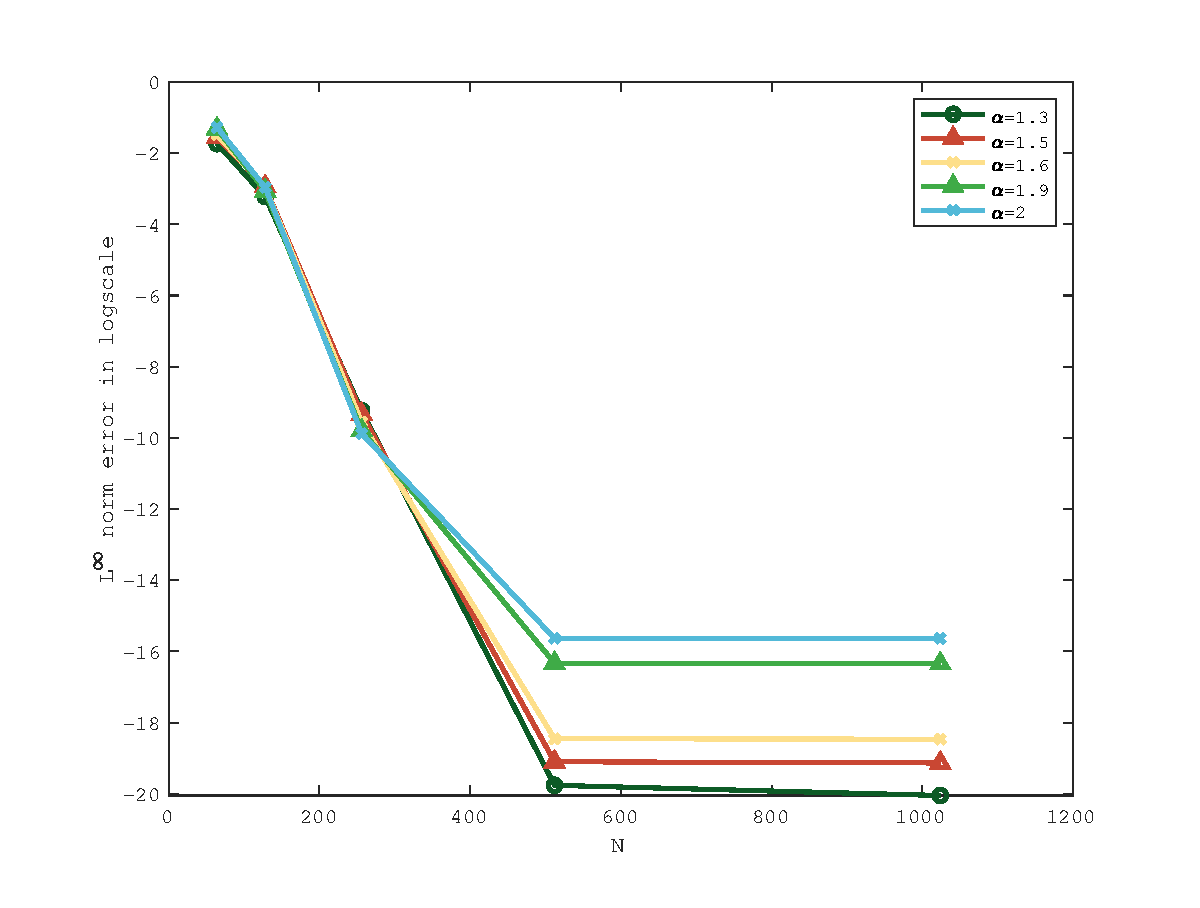
\includegraphics[width=0.5\textwidth]{./figures/exp1_RT_order_s.eps}
% 		%\centerline{($b$) Spatial accuracy with $\tau = 10^{-3}.$}
% 		}\subfigure[$\tau=0.01 $(RT)]{ \centering
% 		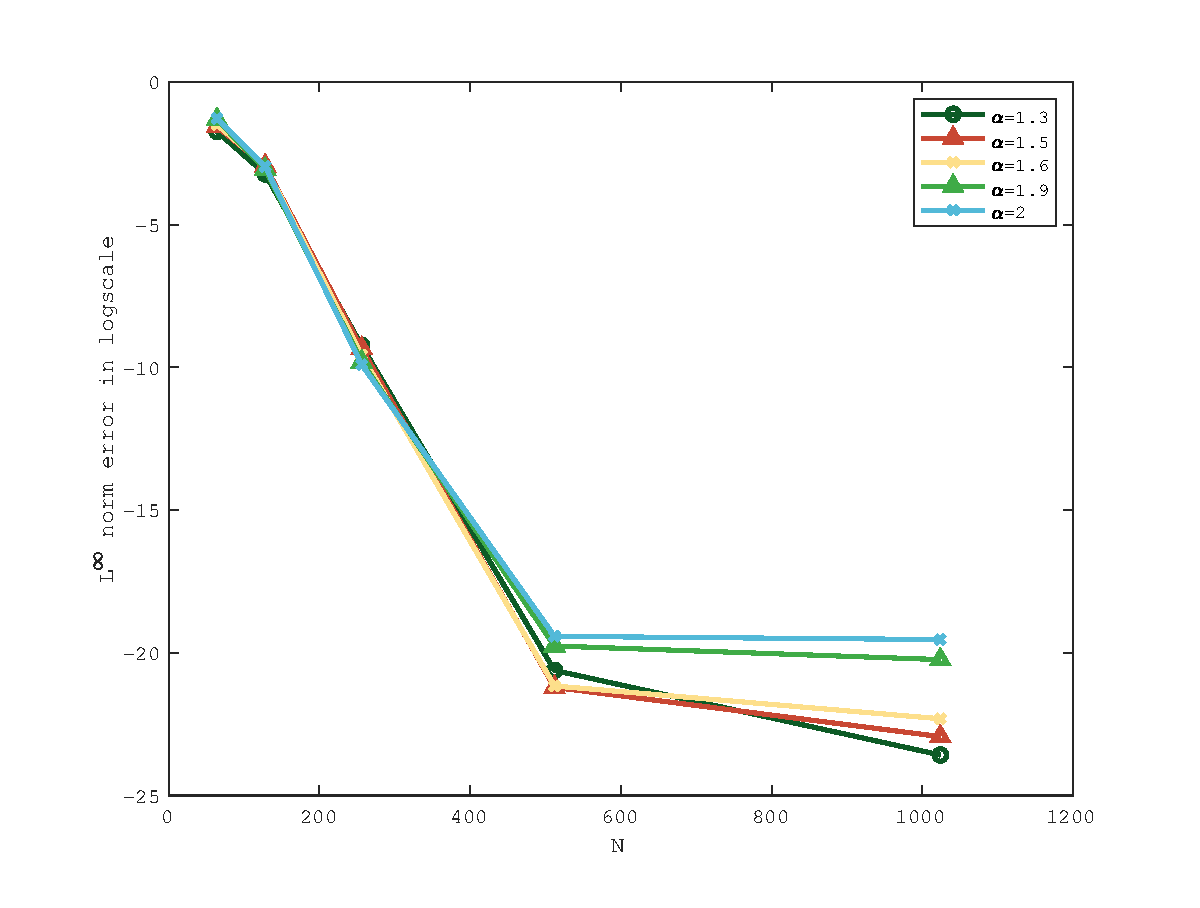
\includegraphics[width=0.5\textwidth]{./figures/exp1_IDT_order_s.eps}
% 		%\centerline{($a$) Temporal accuracy with $N=128.$}
% 		}\caption{不同 $\alpha$ 下 IDT 和 RT 的收敛阶数. (例 \ref{exp_SAVRRK:1})} 
% 		\label{fig_SAVRRK:3}
% 		\end{center}
% 		\end{figure}
% 		我们还进行了一次长时间模拟,直到 $T=1000$,并在图 \ref{fig_SAVRRK:4} 中以不同的 $\alpha$ 绘制了 SAV-RRK(4,4) 方案的相对能量.结果表明,所提出的方案可以在离散场景中完全保持能量,并且其保持效果明显优于 SAV 方案和三级线性隐式差分方案.
%         \begin{figure}[H]
% 		\begin{center}
% 		\subfigure[$\alpha=1.3$]{ \centering
% 		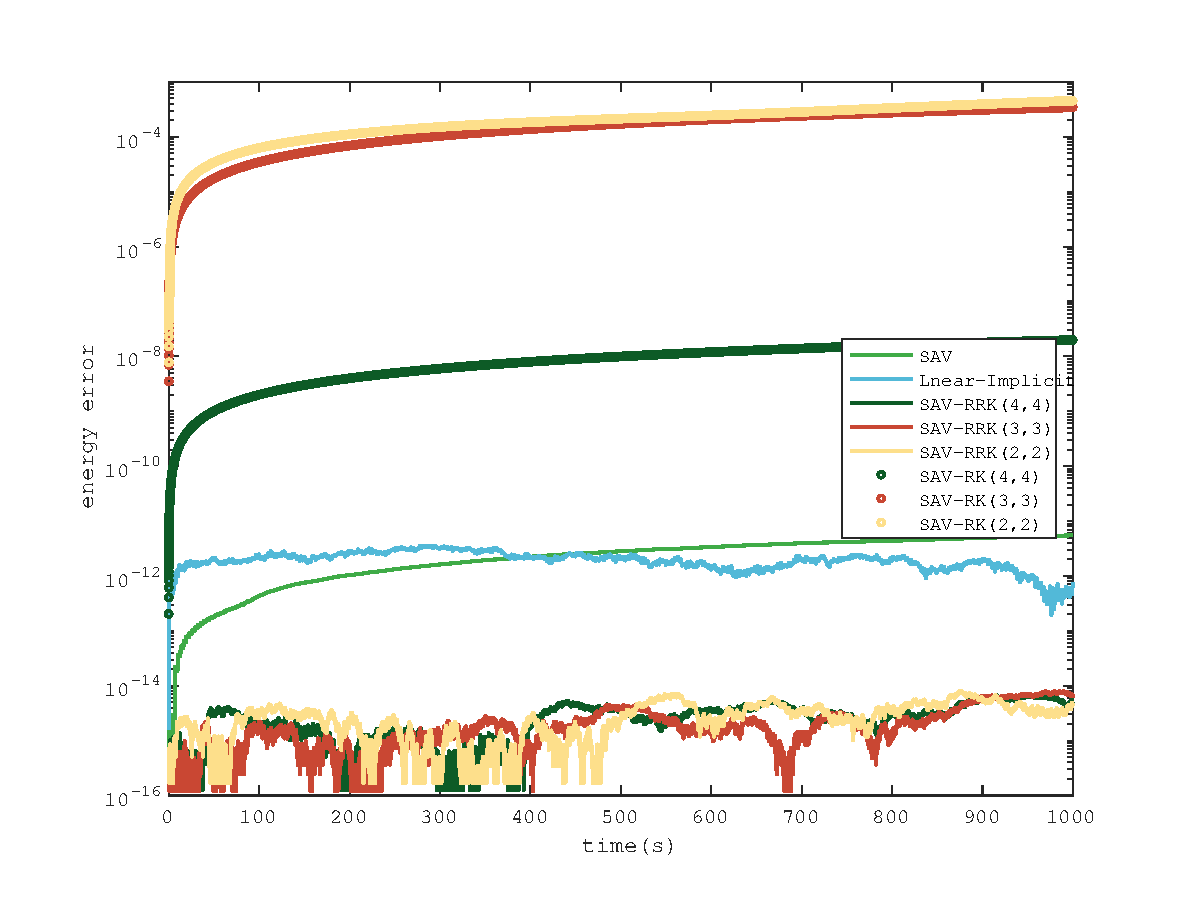
\includegraphics[width=0.5\textwidth]{./figures/exp1_energy3.eps}
% 		%\centerline{($b$) Spatial accuracy with $\tau = 10^{-3}.$}
% 		}\subfigure[$\alpha=1.6$]{ \centering
% 		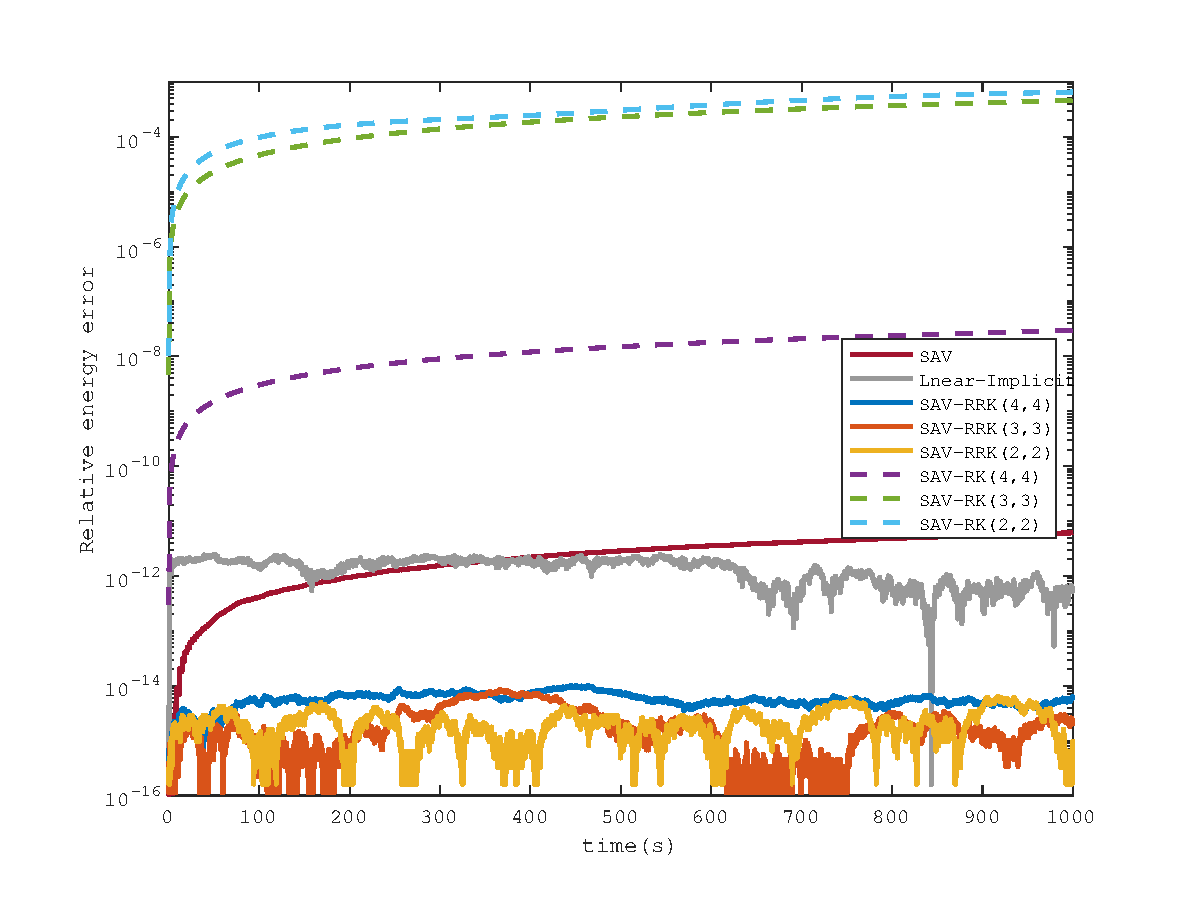
\includegraphics[width=0.5\textwidth]{./figures/exp1_energy6.eps}
% 		%\centerline{($a$) Temporal accuracy with $N=128.$}
% 		}\\
% 		\subfigure[$\alpha=1.9$]{ \centering
% 		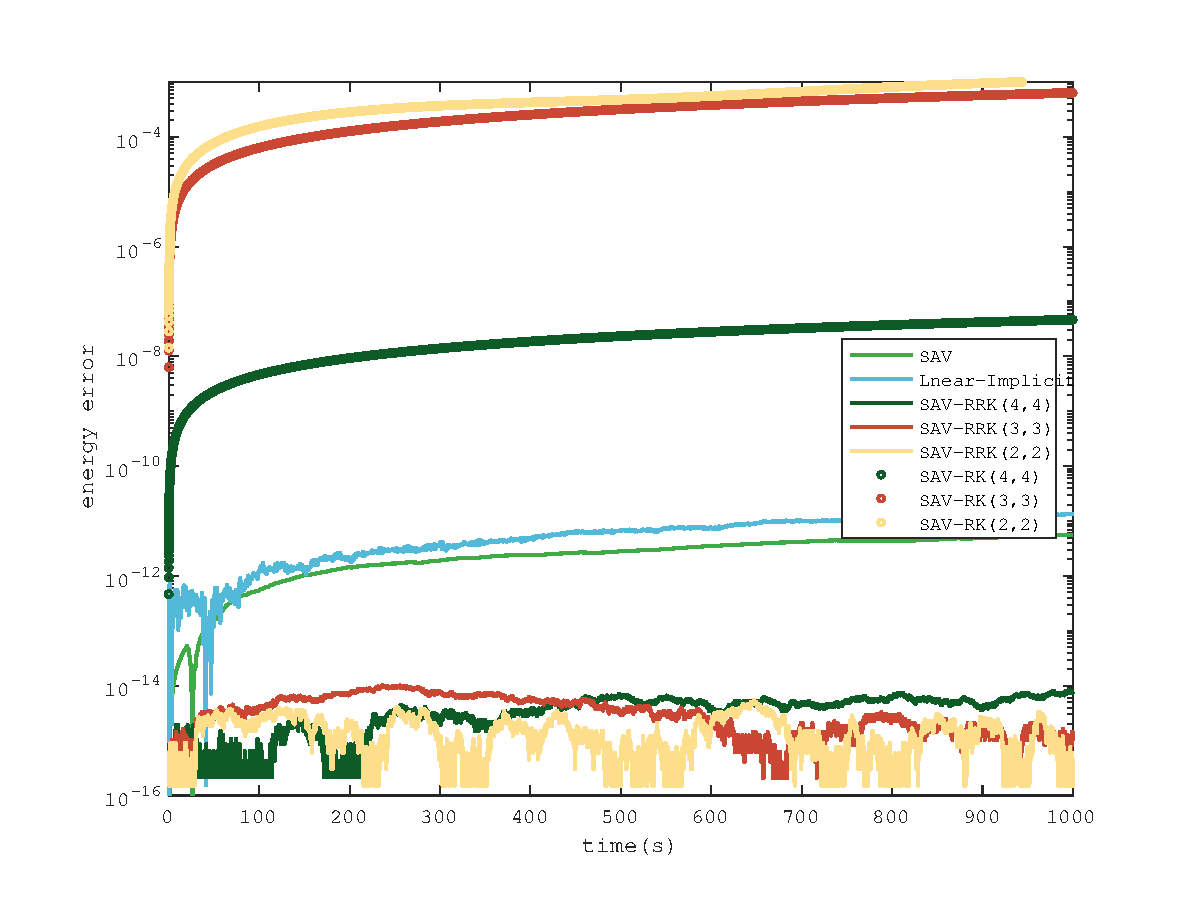
\includegraphics[width=0.5\textwidth]{./figures/exp1_energy9.eps}
% 		%\centerline{($b$) Spatial accuracy with $\tau = 10^{-3}.$}
% 		}\subfigure[$\alpha=2$]{ \centering
% 		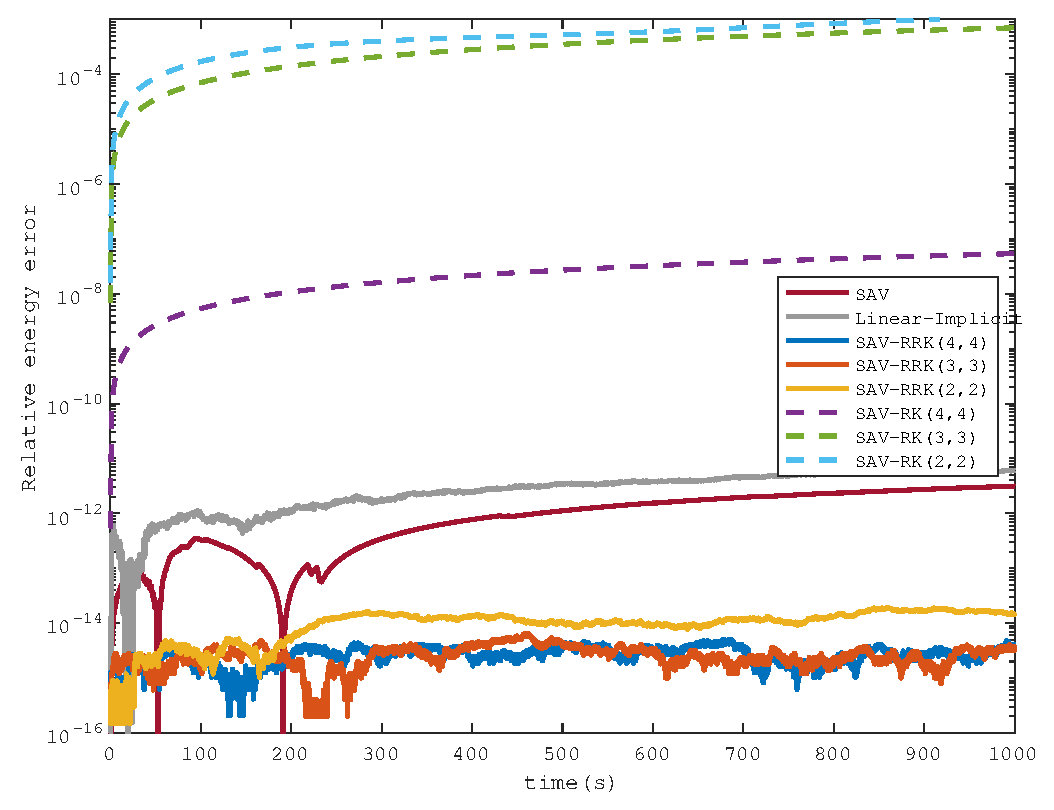
\includegraphics[width=0.5\textwidth]{./figures/exp1_energy2.eps}
% 		%\centerline{($a$) Temporal accuracy with $N=128.$}
% 		}\caption{ 当 $N=32$,$\tau=0.01$ 时,不同 $\alpha$ 下能量的相对误差.(例 \ref{exp_SAVRRK:1})} 
% 		\label{fig_SAVRRK:4}
% 		\end{center}
% 		\end{figure}

% \begin{example}\label{exp_SAVRRK:2}
%     现在我们考虑带有初值的二维 NFSWEs \eqref{eq_SAVRRK:s1}:
% \begin{equation}
% u(x, y, 0)=\operatorname{sech}\left(x^2+y^2\right), u_t(x, y, 0)=\sin (x+y) \operatorname{sech}\left(-2\left(x^2+y^2\right)\right),(x, y, t) \in \Omega \times[0, T],
% \end{equation}
% 其中 $\Omega=[-5,5] \times[-5,5]$.
% \end{example}
